\documentclass{ou-report}
\citestyle{agu}

% Zelf ingezet door John voor de bijlage
\usepackage{pdfpages}
\usepackage{multirow}
\usepackage{subfigure}
\usepackage{stackengine}
\usepackage{afterpage}
\usepackage{longtable}
\usepackage{tablefootnote}
\raggedbottom
% Dit template is gemaakt door P.J. Molijn in het kader van zijn afstuderen aan de OU in 2014.
% Waarvoor hartelijk dank.
% Minieme maar belangrijke wijzigingen zijn aangebracht door E.M. van Doorn
% Het template is versimpeld door Sylvia Stuurman, 2019.


%\hypersetup{
%pdfsubject={Master Thesis <Titel>, <author>},
%pdfkeywords={keyword1, keyword2}
%}

\begin{document}
\pagestyle{plain}
\title[Section Alignment to Detect Document links Efficiently]{SADDLE}
\author{John Stegink}
%Title of the thesis
%\title[Subtitle]{Title}
%\author{author}t
%\affiliation{
%\begin{tabular}{ll}
%Student: & studentnumber \\
%Date:    & DD/MM/YYY \\
%\end{tabular}
%}
%
%%\coverimage{cover/cover.jpg}
%%            ===============
%\makecover[frontboxwidth=4.6in]
\begin{titlepage}

\begin{center}

%% Insert the OU logo at the bottom of the page.
\begin{tikzpicture}[remember picture,overlay]
    \node at (current page.south)[anchor=south,inner sep=0pt]{
        
\includegraphics[scale=0.7]{cover/logo}
    };
\end{tikzpicture}

%% Extra whitespace at the top.
\vspace*{2\bigskipamount}

%% Print the title in specific color.
{\makeatletter
%\titlestyle\color{ou-cyan}\Huge\@title
\titlestyle\color{red}\Huge\@title
\makeatother}

%% Print the optional subtitle in black.
{\makeatletter
\ifx\@subtitle\undefined\else
    \bigskip
    \titlefont\titleshape\LARGE\@subtitle}
\fi
\bigskip
\bigskip

by
%door

\bigskip
\bigskip

%% Print the name of the author.
{\makeatletter
\titlefont\Large\bfseries\@author
\makeatother}

\vfill

in partial fulfillment of the requirements for the degree of
%in overeenstemming met de vereisten voor het verkrijgen van de graad van

\bigskip
\bigskip

{\bfseries Master of Science}

in Software Engineering

\bigskip
\bigskip

at the Open University, Faculty of Science \\
Master Software Engineering
%aan de Open Universiteit Nederland,

to be defended publicly February 15, 2024 at 12:30 PM.

\vfill

\begin{tabular}{lll}
%todo: nog uitzoeken wat hier precies moet komen te staan, wie is chair enz. pagina 34 reader
%% Add additional information here, per faculty requirements, e.g
    Student number: & 835211823 \\
    Course code: & IM9906\\
    Thesis committee:
    	%todo moeten de komma's achter de namen blijven staan?
        & Dhr. dr. Gideon Maillette de Buy Wenniger (chairman) & Open University \\
        & Mw. dr. ir. Clara Maathuis (supervisor) & Open University
\end{tabular}

%% Only include the following lines if confidentiality is applicable.
\bigskip


\bigskip

\end{center}

\end{titlepage} 


%% Use Roman numerals for the page numbers of the title pages and table of
%% contents.
\pagenumbering{roman}
%% Include an optional title page.

\frontmatter 


\let\cleardoublepage\clearpage

% Optional Dedication, Acknowledgement
%\input{dedication}

%\input{acknowledgement}
\tableofcontents

%Optional: list of figures, list of tables
%\listoffigures

%\listoftables

%% Include an optional summary page.
\chapter{Summary}

Finding the correct information is essential to knowledge workers for the optimal performance of their work. They use search engines to find this information in large collections of documents. When documents are found, links to similar documents (semantic links) can help them navigate through this information. Often, subject-related information is only available in knowledge bases with a relatively small set of documents, sometimes in languages other than English. 

Existing research on creating semantic links focuses on small documents written in English and using large sets of documents to train the software. This research aims to overcome these limitations by creating software called SADDLE for creating semantic links in document collections with less than 10K documents in English or Dutch.

SADDLE uses existing text embedding methods to find relations between sections in documents, focusing on performance and the use of computer resources. A neural network is trained to translate the section similarities into document similarities. Existing datasets that can be used to train and test SADDLE were found during this research. However, the datasets are generic and contain only a few documents. To be able to conduct tests on representative document sets, software was created to generate sets of Wikipedia documents about a specific subject using existing Wikipedia-based ontologies and the meta information contained in the Wikipedia hyperlinks. Unfortunately, the quality of the generated document set was too low for training and validation of SADDLE.

When using existing document sets found during research, the conclusion is that SADDLE does not improve the quality of semantic links compared to using the embedding algorithm applied to the total document. SADDLE is not trained optimally because the number of documents in the datasets is low. New research could potentially improve on this limitation by using larger datasets. Creating datasets on a specific subject could probably be improved using metadata other than hyperlinks. Finally, software was created for a user interface to display the relations between sections of documents; this user interface could be improved to be used in knowledge bases. The sources of all created software are publicly available. 


%\input{Summary/samenvatting}

\mainmatter
\pagenumbering{arabic} 

\chapter{Introduction}

When searching for information, users often use search engines like Google\footnote{https://www.google.com} or Bing\footnote{https://www.bing.com}. These search engines have access to a wealth of publicly available information. To make finding the information even simpler and for processing and analyzing it faster, lately, Large Language Models like ChatGPT\footnote{https://www.chatgpt.com} and Google's Bard\footnote{https://bard.google.com} have been developed. The problem with the search engines and the LLMs is that they only have access to publicly available information. Additionally, the LLMs give answers instead of search results. This is very convenient, but the user cannot verify the answer because it contains no references to the sources the information comes from.\\

A source of information that is generally not publicly available is a knowledge base. A knowledge base is a specialized digital library containing documents related to a specific subject. To enable users to find the documents they need, the knowledge bases often contain a search engine that provides a quick and easy method of finding documents. However, users must know what they seek to use a search engine effectively. The search engine's result list only hints at the right documents. This does not account for serendipity, "the finding of unexpected information (relevant to the goal or not) while engaged in any information activity" \citep{andre2009discovery}, which is an important component of information retrieval \citep{foster2003serendipity}. Another drawback is that users are not able to browse through the documents other than via hyperlinks in the text.\\

A way to solve this in a knowledge base is to present links to documents with similar content \citep{makri2014making}. Often, these links are named "Recommended links," "Similar documents," "Read more..." and so on. Figure \ref{imgelsevier} contains an example of a document with links to similar content in a knowledge base. \\


\begin{figure}[h]
\centering
\captionsetup{justification=centering}
\includegraphics[scale=0.197]{images/elsevier.png}
\caption{An arbitrary document from Elsevier Science Direct. The links in the yellow rectangle demonstrate the way semantic links can help users browse through the information.}
\label{imgelsevier}
\end{figure}

Links to documents or parts of documents with similar content are called semantic links. There are various ways to create these links. The most obvious way is to have editors create these links manually. This is, however, a very time and cost-intensive process. Therefore, ideally, these links should be created automatically. The techniques created for the Semantic Web \citep{berners2001semantic} provide a framework using an ontology with which semantic links can be created automatically. This is done using ontologies defining concepts and relations between concepts \citep{Erdmann:2000vn}. Semantic links can be generated by including these concepts in the documents. Subsequently, the relation between the concepts from the ontology can be translated into semantic links. Although links are created automatically, assigning concepts to a document and creating and maintaining the ontologies must be done manually. Semantic links can also be created without manually manipulating the content. This can be done using artificial intelligence (AI) models that "understand" the natural language. Modern versions of such models need many documents (more than 100K documents) to be trained and a lot of computer resources to work.\\

Because a knowledge base typically contains no more than 10K documents, and topics in a knowledge base come with their own jargon and specialized terms, or the documents are written in a language other than English, models that were trained on content from general texts or content from other knowledge bases ignore this special information and therefore cannot generate optimal semantic links. Ideally, a specialized model must be created for each knowledge base.

Another property of knowledge bases is the limited number of potential users. If a knowledge base is to be used commercially, the amount of computer resources that can be allocated is limited to constrain the operating costs. This creates a need for models that can be trained on fewer than 100K documents and are resource-efficient.\\

The research conducted for this thesis aims to overcome the previously mentioned obstacles: large training sets, using languages other than English, and limited resources. Software is created to use an enhanced version of the large-scale hierarchical alignment (LHA) algorithm \citep{nikolov2018large}. This software is named SADDLE (Section Alignment to Detect Document Links Efficiently). Where the LHA algorithm is designed for aligning sentences in documents, SADDLE finds similarities between sections and documents. Both algorithms are constructed to work with 10K documents or less and are scalable.\\

A key success factor for SADDLE is to use good training and validating sets. One option is to create the sets using ontologies that were produced for the Semantic Web and to combine these ontologies with articles from Wikipedia.\\

The above leads to the following main research question of this thesis: \textit{How can hierarchical decomposition into sections and encoding help find automated relations between documents or sections in document sets that contain less than 10K documents?}

To answer this question, the CRoss-Industry Standard Process for Data Mining (CRISP-DM) research method\footnote{https://www.datascience-pm.com} is used. Firstly, this means that at least one, preferably more representative training- and validation sets must be found or created. Secondly, the SADDLE algorithm is improved in several steps. Every step is validated to determine the quality of the improvement. A detailed description of the research method is given in section \ref{secResearchMethod}.  \\

This thesis is structured as follows. Chapter \ref{sectRelatedWork} overviews research on semantic relations between documents. The research question, the subquestions, the research method, and how the research is conducted and validated are outlined in section \ref{secResearch}. Chapter \ref{secRCI_II} elaborates on the datasets that are publicly available at this moment. An attempt was made to create a topic-based dataset (chapter \ref{chapTopicDatasets}). The results of experiments using the SADDLE algorithm can be found in chapter \ref{secResults}. The last chapter, chapter \ref{secConclusions}, contains the concluding remarks, identified limitations, and possible future work perspectives.



\pagebreak
\chapter{Related work \& Research background}
\label{sectRelatedWork}
\label{sectBackground}


In the first sections of this chapter, an overview of the research conducted into semantic relations between documents will be given.  Natural Language Processing (NLP) is the area of Artificial Intelligence (AI) research that focuses on understanding, reading, and responding to human language. An introduction to NLP and several concepts used in this thesis is given in \citep{rao2019natural} and \citep{Goodfellow-et-al-2016}. This section discusses the context/background of this research and related studies. 

The last sections contain a theoretical background that was used during the research. These sections are meant as an introduction to the theory and help understand the research for this thesis.\\

\section{Text embeddings}

One of the subfields of NLP is to create embeddings of a document or part of a document. An embedding is a numerical representation of a text that contains the essence of the text and is represented as vectors with real numbers. Text embeddings can be used for a wide range of applications.

 Using the embedding vectors, the similarity between the texts can be calculated; a method often used to accomplish this is cosine-similarity, which has the feature that the larger the cosine-similarity is, the more similar the texts are. An example of vector embeddings of documents $A$, $B$, and $C$ is given in figure \ref{imgcossim}. For this example, the vectors are simplified to two dimensions to be shown in an image. The angle $\alpha$ is smaller than angle $\beta$, i.e. $\cos(\alpha)$ is larger than $\cos(\beta)$.  Because the embedding is a representation, the smaller the cosine between the embedding vectors, the more similar the documents are. In the example, documents $A$ and $C$ are more related than $A$ and $B$ or $B$ and $C$.

\begin{figure}[h]
\centering
\captionsetup{justification=centering}
\includegraphics[scale=0.3]{images/cosine.png}
\caption{A two dimensional example of cosine-similartiy.\\Vector A en C are more similar than A and B or C and B.}
\label{imgcossim}
\end{figure}



Text embeddings can be created using statistical methods, of which Term Frequency, Inverted Document Frequency (TF-IDF) \citep{robertson2004tdidf} is one of the most well-known methods. The intuition behind TF-IDF is that a word is a significant term for the text when that term is frequently used in the text, but its average usage in other documents is much lower. This way, a text can be represented as a vector containing this ratio (document frequency and total frequency) for every term.\\

Another method for creating embeddings of texts is to sum up, or average, the embeddings of all the individual words in a document. Embeddings of words with similar meanings have similar vectors, and math operations can be performed with these vectors to a certain extent, for example, $King - Man + Woman = Queen$. Word embeddings are often pre-calculated on a large corpus of documents. A word embedding is determined by analyzing which words frequently co-occur with others; examples of algorithms that create word embeddings are Word2Vec \citep{mikolov2013distributed} and Global Vectors for Word Representation (GloVe) \citep{glove}.  \\

Semantic hashing can efficiently find related documents in a production environment \citep{semantichashing}. Semantic hashing means a deep graphical model learns word-count vectors from a large document set. The values of the deepest layer are used to represent the documents. When the deepest layer uses a small number of variables, this is mapped to a number using the values as bits. When documents are semantically similar, the difference between the numbers is small, and this property can be used to find related documents quickly. The binary codes are compared simply when the deepest layer uses more variables.\\
  
Another way to find relations between documents in a production environment with many variables is by using a nearest-neighbor search algorithm instead of finding the nearest neighbors of a document by comparing the relative distance to all other documents. As defined by WikiPedia\footnote{https://en.wikipedia.org/wiki/Nearest\_neighbor\_search}: "Nearest neighbor search (NNS), as a form of proximity search, is the optimization problem of finding the point in a given set that is closest (or most similar) to a given point. Closeness is typically expressed in a dissimilarity function: the less similar the objects, the larger the function values." A prevailing and fast implementation of a nearest neighbor search algorithm is ANNOY (Approximate Nearest Neighbors Oh Yeah)\footnote{https://github.com/spotify/ANNOY}

\section{Transformers}
The problem with using word embeddings is that the context of the sentence in which the word occurs is ignored. Considering the sentences "The man was accused of robbing a \textit{bank}." and "The man went fishing by the \textit{bank} of the river." the word \textit{bank} has a different meaning. The word's meaning is determined by its context, i.e., the other words and the place in the sentence. \\

Neural networks are an excellent way to determine patterns in data. The neural network architecture is inspired by the neurons in the brains of humans. They contain an input layer, one or more hidden layers, and an output layer. The nodes connect and have an associated weight and threshold. The neural network calculates the values of these weights and thresholds during the training phase. Detailed information about neural networks can be found in literature, for example, \citet{rao2019natural}. For an explanation of training neural networks, see section \ref{secTrainingNeuralNetworks}.\\

These neural networks can help to solve the problem of finding the correct meaning of a word within its context. Examples of these neural networks are sequence-to-sequence (S2S) models, a special case of a general family of models called encoder–decoder models ~\citep{boekh8}. An encoder–decoder model takes a text sequence (often a sentence) and encodes this text as a numeric (vector) representation. This representation is fed into a decoder that decodes the numeric representation as a new text similar to the original text (as depicted in figure \ref{imgs2s}). 

\begin{figure}[h]
\centering
\captionsetup{justification=centering}
\includegraphics[scale=0.7]{images/s2s.png}
\caption{Sequence to sequence model. The original text is encoded first and then decoded into a new text. The model learns by comparing the original text with the new text.}
\label{imgs2s}
\end{figure}

This model is often used for the translation of texts from one language to another (for example, English to Dutch) or from one writing style to another.\\

  As building blocks of these encoder-decoder models, different kinds of recurrent neural networks (RNN) \citep{rnn} are being used. An RNN is a neural network that has an internal state (memory) and can process input sequences. Examples of RNNs that are often used for sequence-to-sequence networks are: Long Short Term Memory recurrent neural networks (LSTM) \citep{lstm} and gated recurrent units (GRU) \citep{gru}.\\


A new type of encoder-decoder model is the transformer model \citep{vaswani2017attention}, which performs better than encoder-decoder models based on RNNs. A particular mechanism for the transformer model is depicted in Figure \ref{imgtransformer}. Besides the description by \citep{vaswani2017attention} a good explanation of the model is given in “The Annotated Transformer.”\footnote{https://nlp.seas.harvard.edu/2018/04/03/attention.html}. \\

A transformer is superior in quality compared to sequence-to-sequence models based on RNNs. A transformer can be computed parallel, whereas an RNN can only be computed sequentially. Both the encoder and the decoder of the transformer model have a somewhat different yet similar structure centered around the use of (self-)attention. They each consist of six repeated and identical layers, which differ slightly between the encoder and decoder due to the addition of the output in the decoder. Importantly, the (self-)attention mechanism in these layers is done for all combinations of words/elements in the processed sequences.  This causes the computational complexity of these layers and, hence, the whole network to become 
quadratic in the sequence length. In contrast, the computational complexity of RNNs is linear in the sequence length. That means a transformer uses much more computation, but if the sequence length is limited and parallelization is used, it is less of a problem. The pairwise comparison ensures that every word is compared, irrespective of the distance between the words in the pair.  The RNN compares the words indirectly by using the memory state, which has a limited capacity and can leak information. This is why transformers can exploit the full sequence context much better than an RNN.

\begin{figure}[h]
\centering
\captionsetup{justification=centering}
\includegraphics[scale=0.2]{images/transformer_model.png}
\caption{The architecture of the transformer model, a very popular sequence to sequence model.}
\label{imgtransformer}
\end{figure}


One of the state-of-the-art techniques, based on the transformer model, is BERT: Bidirectional Encoder Representations from Transformers \citep{devlin2018bert} and the improved version of BERT, the Robustly Optimized BERT Pre-training Approach (ROBERTA) \citep{Liu2019RoBERTaAR}. These models create word embeddings based on the word's context within the sentence and can learn the relation of two consecutive sentences by Next Sentence Prediction (NSP). The models can be used as a filtering network, which means they can be used as a building block for new models. Pre-trained models of BERT and ROBERTA are available for many languages. Bertje \citep{devries2019bertje}, a BERT model, and RobBERT \citep{delobelle2020robbert}, a RoBERTa model, are examples of pre-trained models that are available for the Dutch language for example.\\


Next to word embeddings and relations between consecutive sentences, the BERT model has an output that can embed a single sentence. The quality of this sentence embedding could be better; an average of GloVe \citep{glove} word embeddings are often better \citep{reimers2019sentence}. To find similar sentences in a collection of 10K documents using a pairwise comparison with BERT would take up to $\frac{1}{2}.n.(n-1)$ computations (this would take 49~ 995~000 inference computations), requiring up to 65 hours of computation time). \\

The Universal Sentence Encoder (USE) is an embedding method \citep{cer2018universal} to calculate embeddings of texts of arbitrary size, although it is most suitable for short texts, like sentences.  USE is a model toolkit containing two algorithms: a deep averaging network (\textsc{DAN}) \citep{DAN} and an algorithm that uses the transformer architecture. The transformer-based sentence encoder performs as well or better than the DAN encoder. The DAN-based sentence encoder generally gives better results.\\

 The algorithm Sentence BERT \citep{reimers2019sentence} uses a siamese network \citep{jiang2019semantic} containing BERT and RoBERTa models to create sentence embeddings. The embeddings of 10K documents can be computed in approximately 5 seconds, and by using cosine-similarity, the comparison would take about 0.01 seconds. These embeddings outperform other state-of-the-art sentence embedding methods like InferSent \citep{conneau2017supervised} and Universal Sentence Encoder \citep{cer2018universal}, by 2.1 and 2.6 points, respectively, on SentEval \citep{conneau2018senteval}.
 
\section{Aligning}
\label{sectAligning}

Text aligning is used for NLP tasks like generating sentence pairs for model training, detecting plagiarism, finding comparable documents, and making citation recommendations. Aligning texts makes it possible to find similar parts in different documents. Such text parts can be corresponding sentences, paragraphs, or sections. The encoding process is one of the critical components of an NLP system to align texts \citep{zhou2020multilevel}. 

Hierarchically structured document encoders, of which Hierarchical Attention Networks (HAN) \citep{yang2016hierarchical} are often used implementations and are neural networks that combine Word2Vec \citep{mikolov2013distributed} vectors into sentence embeddings. These embeddings, in turn, are combined to be used as a document embedding. \citet{jiang2019semantic} use a HAN in a siamese network \citep{mueller2016siamese} to learn whether there is a relationship between two documents.\\


Because the system as described by \citet{jiang2019semantic} ignores structural correspondence between parts, \citet{zhou2020multilevel} propose a new approach: "Multilevel Text Alignment with Cross-Document Attention." The authors propose a deep neural network that can predict relationships across different document levels. These levels are document-to-document and sentence-to-sentence.

\begin{figure}[h]
\centering
\captionsetup{justification=centering}
\includegraphics[scale=0.22]{images/mta}\caption{Architecture of the multilevel Text Alignment with Cross-Document Attention model.}
\label{imgmta}
\end{figure}

The structure of the model is shown in Figure \ref{imgmta}, where $x_i$ represents a word, $s_j$ represents a sentence, and $d_l$ represents a document. The contextualizer does the aggregation of the words into a sentence. This is a sub-network that takes the importance of the words (attention) into account. The aggregation of the sentences into the document is done similarly. The blue lines in the figure denote the cross-document attention. This can either be \textsc{Shallow} (without the dashed lines) or \textsc{Deep} (including the dashed lines).

The resulting model is a very deep neural network, especially the \textsc{Deep} version of the model. This means that it takes a lot of time and a lot of documents to be trained properly. \citet{zhou2020multilevel} conducted several experiments wherein the training took up to 48 hours for the most complicated model. The authors found that document-to-document relations are not optimal: "which could be attributed to the small size of the plagiarism dataset" when used with a dataset containing 23K documents. Other experiments that were conducted do not have this restriction. The datasets for these experiments consist of more than 130K documents. \\

\citet{nikolov2018large} describe an algorithm to create sentence alignments, called the "Large-scale hierarchical alignment (LHA)" algorithm. First, their algorithm computes the embeddings of all documents and finds similar ones using the nearest neighbors. They use several methods for computing the document embedding and compare the performance of the methods in their paper. Second, the nearest neighbors of the sentences of the previously found document pairs 
 are computed and used for the sentence alignment. The authors find \textit{Sent2Vec} \citep{pagliardini2017unsupervised} to be the fastest to compute and perform well on document embedding and sentence alignment. The authors state that "LHA is robust to noise, fast and memory efficient, enabling its application to datasets on the order of hundreds of millions of sentences." 

One of the reasons that the algorithm is fast to compute is that it divides the computation of sentence embeddings into two hierarchical steps. First, the algorithm computes document embeddings. This can be done fast but with less precision. The precision is unimportant because it is used for filtering the documents to be compared. The filtering, however, dramatically reduces the number of sentences to be compared (figure \ref{imgQP}), which must be precise and is thus less fast. Second, the algorithm aligns the sentences of the filtered documents.\\

\begin{figure}[hbt]
\centering
\captionsetup{justification=centering}
  \includegraphics[scale=0.6]{images/Quality_vs_performance.png}
  \caption{Quality vs Performance}
  \label{imgQP}
\end{figure}


Table \ref{tabAlgorithms} gives an overview of the algorithms described in the previous sections. The first column contains the name of the algorithm in the family of algorithms. The second column includes the year it was described for the first time. The third column contains "Yes" when the algorithm is based on a neural network and is used as such\footnote{The algorithm used pre-trained models that can be neural networks, but the algorithm itself is not a neural network}. The last column is "Yes" when pre-trained models are available for this algorithm.


\begin{table}[h!tbp]
    \centering
    \captionsetup{justification=centering}
    \begin{tabular}{p{7.5cm}|l|l|l}
    	\textbf{Algorithm} & \textbf{Year} & \textbf{Neural} & \textbf{Pretrained} \\ 
    	& & \textbf{network}\\
		\hline
        TF-IDF & 2004  & No & No   \\
		\hline
        Word embeddings & &  \\
		\hline
        \hspace{3mm}Word2Vec & 2013 & Yes & Yes \\ 
		\hline
        \hspace{3mm}GloVe & 2014 & Yes & Yes \\ 
		\hline
        Encoder-decoder & 1987 & \\
		\hline
        \hspace{3mm}LSTM & 1997 & Yes & No   \\ 
		\hline
        \hspace{3mm}GRU & 2014 & Yes & No \\
		\hline
        Transformers & 2017 & & \\
		\hline
        \hspace{3mm}BERT & 2019 & Yes & Yes  \\
		\hline
        \hspace{3mm}RoBERTa & 2019 & Yes & Yes  \\ 
		\hline
        \hspace{3mm}Sentence BERT & 2019 & Yes & Yes   \\ 
		\hline
        Deep Averaging Network (DAN) & 2016 & \\ 
		\hline
        \hspace{3mm}Universal Sentence Encoder & 2018 & No &  Yes \\
        Hierarchical Attention Networks (HAN) & 2016 & \\ 
		\hline
        \hspace{3mm}Multilevel Text Alignment with & 2019 & Yes &  No \\
        \hspace{3mm}Cross-Document Attention & 2020 & & \\ 
		\hline
        \hspace{3mm}Large-scale hierarchical alignment (LHA) & 2018 & No & No  \\ 
		\hline
    \end{tabular}
    \caption{An overview of the discussed algorithms used for embeddings and alignment.}
  	\label{tabAlgorithms}
\end{table}




\section{Text corpora}

A large number of systematically collected structured texts is called a text corpus. In NLP, corpora are used for training an algorithm, validating an algorithm, and for benchmarking. Many corpora exist, most in English, but corpora in other languages are also available. Common Crawl\footnote{http://commoncrawl.org}, for example, contains texts in over 40 languages. To be useful as a corpus for algorithms that determine semantic relations between texts, the corpus has to contain annotations about relations between the texts. Most of the existing corpora do not provide such information.\\

A source for texts to be used in NLP is scientific (academic) papers, but these come with limitations. First, scientific papers are always available in the PDF format. A PDF is a graphical format; extracting text from the PDF is no trivial feat. \citet{kdir20} state that "... tools for extracting text from PDF documents would often mix body and non-body texts." The authors created a tool that recreates the text as closely as possible but does not preserve the document structure. A way to circumvent the problem is to use a LaTeX source, but not all papers are written with LaTeX software, and when they are, the sources are not always available. The second limitation is that scientific papers are not always free. Third, scientific papers are mostly written in English. On the positive side, because scientific papers contain references to other scientific papers, a semantic relation between papers can be determined using citation- or hyperlink-based approaches.\\

Another source of text to be used for NLP corpora is Wikipedia. It is freely available in many different languages\footnote{https://en.wikipedia.org/wiki/List\_of\_Wikipedias\#Details\_table}. Dumps containing all articles written in a particular language can be downloaded for free. Hyperlinks can determine the relation between the articles and other articles in the text of an article.

Instead of links between articles, ontologies containing semantic relations between concepts from Wikipedia can be used for article relations. For example, DBPedia \citep{BIZER2009154} and Wikidata \citep{vrandevcic2014Wikidata} are large ontologies available for free. \citet{ostendorff2020pairwise} use the Wikidata ontology because it is "an open knowledge graph in which nodes represent items (e.g., Wikipedia articles) and edges represent properties of these items (e.g., a relation that connects two different articles)." The authors only use a set of properties as a relation and conclude that Wikipedia, in combination with an ontology, is suitable to be used as a corpus for algorithms that determine semantic relations between texts.\\

\section{F1 Score}
\label{F1Score}
Evaluation metrics quantify the quality of the semantic links generated by an algorithm. They can be used to compare the quality of various algorithms and help improve an algorithm while it is in development. The F1 metric \citep{forman2003} is an often-us evaluation metric in NLP research. It is a measure of an algorithm’s accuracy on a dataset, represented by the formulas \ref{eqF1a}, \ref{eqF1b} and \ref{eqF1c}.

\begin{subequations}
\begin{equation}
\label{eqF1a}
F1 = \frac{ 2 \times recall \times precision}{recall + precision}\end{equation}
\begin{equation}
\label{eqF1b}
precision = \frac{|\{relevant\ documents\}\  \cap\  \{retrieved\ documents\}|}{|\{retrieved\ documents\}|} 
\end{equation}
\begin{equation}
\label{eqF1c}
recall = \frac{|\{relevant\ documents\}\  \cap\  \{retrieved\ documents\}|}{|\{relevant\ documents\}|}
\end{equation}
\end{subequations}\\


In a classification context, values for precision and recall can be calculated with the formulas \ref{eqF1d} and \ref{eqF1d}, where \textit{tp} denotes the \textit{true positives}, \textit{fp} the \textit{false positives} and.  \textit{fn} the \textit{false negatives}.\\

\begin{subequations}
\begin{equation}
\label{eqF1d}
precision = \frac{tp}{tp + fp}
\end{equation}
\begin{equation}
\label{eqF1e}
recall = \frac{tp}{tp + fn}
\end{equation}
\end{subequations}\\


\section{Ranking}
\label{ranking}
Semantic link generation can be considered a classification problem, meaning a valid result in the generated links and the validation data is considered a true positive. However, it is more specifically a ranking problem in which the most relevant semantic links must not only be retrieved but also placed at the top of the ranking. \cite{Rajaram2003} argue, "If the ranking problem is posed as a classification problem, then the inherent structure present in ranked data is not used of, and hence generalization ability of such classifiers is severely limited.".   The generation of semantic links can also be viewed as a ranking problem for search, with the document being the query and the semantic links representing the search results. \\

By using precision at K (P(K)), \citep{Agichtein2006} an F1 score can be calculated for this ranking problem. P(K) reports the fraction of documents ranked in the top K results labeled as relevant. The position of relevant documents within the top K is irrelevant. This can be described mathematically as:
$$precision = \frac{l}{c},\ \ \ \ recall = \frac{l}{t}$$ where \textit{l} denotes the \textit{the number of recommended items of the top K results that are relevant}, {c} denotes the \textit{the number of recommended items of the top K results} and \textit{t} denotes the \textit{total number of relevant items}. A detailed explanation with examples can be found on Medium.com\footnote{https://medium.com/@m\_n\_malaeb/recall-and-precision-at-k-for-recommender-systems-618483226c54}.\\

The Spearman correlation coefficient\footnote{https://en.wikipedia.org/wiki/Spearman\%27s\_rank\_correlation\_coefficient}
 and Kendall correlation coefficient\footnote{https://en.wikipedia.org/wiki/Kendall\_rank\_correlation\_coefficient} are other often used metrics for calculating whether a list of items, in this case, semantic links, have the correct order of significance. The ranking is more important than the absolute value of an item in case of finding semantic links. The Spearman correlation and the Kendall coefficient are between -1 and 1, where a higher value denotes a higher correlation. These are statistical coëfficents of which the theory is out of the scope of this thesis. \citet{APCCoefficient} propose a new correlation coefficient, the AP Correlation Coefficient (APC). The APC pays more attention to the higher-ranked items than the lower-ranked items. Both the Spearman and Kendall correlation treat these equally.\\

To use ranking values as a metric, it is necessary to have a list with the desired ranking for each document pair. This is often not easy to realize, and therefore, the ranking matric is not often used.


\section{Wikidata \& DBPedia}
\label{sectWikidataDBPedia}

Wikidata \citep{vrandevcic2014Wikidata} and DBPedia \citep{dbpedia} are knowledge graphs linked to Wikipedia articles and can potentially be used for generating suitable datasets. The DBPedia knowledge graph is created by extracting structured content from Wikipedia information. On the other hand, the knowledge graph created by the Wikidata project serves as an information source for projects like Wikipedia. Hence, DBPedia uses Wikipedia as a source of information, while Wikidata serves as a source for Wikipedia. This makes Wikidata more appropriate for creating datasets since the text from Wikidata doesn't always need to be included in the final Wikipedia article. The Wikidata knowledge graph is less dependent on the information and structure of the Wikipedia article than DBPedia.\\

Wikidata is a knowledge graph that is multilingual by design and is published under legal terms that allow the broadest possible reuse \citep{vrandevcic2014Wikidata}. Information from Wikidata can be represented as semantic triples in the form of Resource Description Format (RDF) triples \citep{erxleben}. RDF triples are a standardized way to describe information. They are in the form \texttt{<subject, predicate, object>}. For example, the triple \texttt{ <dog, produced sound, bark>} indicates that a dog can make a barking sound. Because Wikidata is multilingual by design, IDs represent the elements of the triple that can be translated into a description in one of the many languages supported by Wikidata. The Wikidata RDF triple \texttt{<wd:Q144, wdt:P4733, wd:Q38681>} describes the previous example.\\ 


\section{Wikipedia subgraphs}
\label{secWikipediaSubgraphs}
\citet{Ponza2017} conducted a "study of all entity relatedness measures in recent literature based on Wikipedia as the knowledge graph." In their study, they devised a system for calculating a relatedness measure between two Wikipedia articles. The study found the  CoSimRank algorithm \citep{cosimrank} to be a good measure for calculating this. The disadvantage of this algorithm is that it does not perform well on large graphs like the Wikipedia article graph. To overcome the performance problem, a small subgraph is constructed consisting of articles close to the original articles. The CosSimRank algorithm uses this subgraph to perform its calculations \citep{cosimrank}. \\

The system devised by \citet{Ponza2017} is too complicated to be implemented for this thesis. It would have taken too much time and resources. For constructing the previously described subgraph, \citet{Ponza2017}, have analyzed several algorithms that use either the text of the article or its hyperlinks. The authors found that one of the best methods using the hyperlink structure of Wikipedia is the Milne\&Witten score described by \citet{Witten2008} or DeepWalk, described by \citet{deepwalk}. The Milne\&Witten score can be calculated easily and quickly without spending too much time. For these reasons, this score was chosen over the CoSimRank or Deepwalk algorithms to implement in this thesis. Formula \ref{formulaMilneWitten} contains the formula for calculating the Milne\&Witten score.\\

\begin{equation}
\captionsetup{justification=centering}
\label{formulaMilneWitten}
1 -\frac{ log( max( |A|, | B| )-log(| A \cap B|))}{log(|W|)-log(min\{|A|, |B|\})}
\end{equation}
\\ 
The formula \ref{formulaMilneWitten} calculates the Milne\&Witten score, where a and b are the two articles of interest, A, and B are the sets of all articles that link to a and b, respectively, and W is the entire Wikipedia.

\section{Training neural networks}
\label{training}
\label{secTrainingNeuralNetworks}
Neural networks need a dataset to be trained. To properly train a model and assure proper learning and performance, the dataset is split into three datasets: a training set, a validation set, and a test set (See figure \ref{imgTrainValidationTest}). Firstly, the basic training of the parameters of a model is done using the training set. Secondly, the model is trained several times to determine the optimal hyperparameter configuration. The validation set is used to find the most optimal configuration by selecting the configuration with the lowest error on the validation set. Lastly, the test set is used to determine the model's performance. This set cannot be the same as the validation set because the validation set was used to determine the configuration of the model and, therefore, can be biased. In research, 60\% of the dataset is often used as a training set, 20\% as a validation set, and 20\% as a test set; depending on the size of the dataset, these values can change.\\

\begin{figure}[h]
\centering
\captionsetup{justification=centering}
\includegraphics[scale=0.75]{images/Datasetsplit.drawio.pdf}
\caption{A dataset is split into separate sets for training, validation and test purposes.}
\label{imgTrainValidationTest}
\end{figure}


When dataset size is relatively low, it is essential to make optimal use of the dataset. As mentioned above, splitting it into three sets makes even fewer items available for training. K-Fold Cross-Validation is an often-used method to use all values for training without "losing" values for validation. With this method, the dataset is split into K folds, where one is used for validation, and K-1 folds are used for training. In the next iteration, another fold is used for validation, and the remaining folds are used for training. This process is repeated K-times until all folds are used for validation. The final result of the training is the average of the accuracy and F1 value of all iterations. Using K-Fold Cross-Validation, the relatively small number of training examples available in Wikisim and WiRe is used efficiently. This advantage compensates for the increased computer resources needed to train the neural network. A graphical representation of K-Fold Cross-Validation is depicted in figure \ref{imgKFold}.  
\\

\begin{figure}[h]
\centering
\captionsetup{justification=centering}
\includegraphics[scale=0.25]{images/kfold.png}
\caption{Schematic overview of K-fold Cross-Validation with K=5. (The image was copied from \\https://towardsdatascience.com /cross-validation-k-fold-vs-monte-carlo-e54df2fc179b).}
\label{imgKFold}
\end{figure}\\

It is called overfitting when a neural network produces good results on the training but not the test set. This means the model learned too well from the training data but cannot perform well on the unseen data. Hence, the model is not able to generalize well. Overfitting typically occurs when:
\begin{itemize}
  \item The training data size is too small and does not contain enough data samples to accurately represent all possible input data values.
  \item The training dataset includes a significant amount of irrelevant information.
  \item Because of the high complexity of the neural network it learns on invalid data in the training data.
\end{itemize}\\

To mitigate overfitting the following (not extensive) list of options is available:
\begin{itemize}
\item \textbf{Pruning}: Decrease the number of features in the data, so less parameters are needed in the network.
\item \textbf{Regularization}: Add "noise" to the data by mathematical computations in order to make the network more rebust.
\item \textbf{Data augmentation}: Artificially create extra data based on the data in datasets.
\end{itemize}





\pagebreak
\chapter{Research approach}
\label{secResearch}

Creating semantic relations between documents is beneficial for information retrieval and information recommendation. When used in a knowledge base, a data repository containing information about a specific topic, it can help users find the necessary information. Users can use the semantic relations to navigate through the knowledge base.\\

The available algorithms mostly cannot be used for knowledge bases. Firstly, although very large knowledge bases exist, they are often small in practice because they contain information about a specific topic on which not necessarily many documents are available. Most existing algorithms require many documents to be trained (more than 100K documents). Secondly, not all knowledge bases are in English, but they sometimes contain information in another natural language and, therefore, most of the time, have fewer documents. A model that can be trained on a smaller set of documents is better suited to these knowledge bases. Using a model trained on documents contained in the knowledge base is the most optimal because it is tuned to the specific topic of the knowledge base. \\

The large-scale hierarchical alignment (LHA) algorithm \citep{nikolov2018large}, as mentioned in section 2.3, is a suitable algorithm for creating semantic relations between knowledge base documents.
Although the LHA algorithm was created to extract parallel sentence pairs instead of similarities of sections and documents, it can be used as a base for a new yet-to-be-created algorithm (SADDLE) that extracts parallel section pairs. The information of the section pairs can be used for two purposes. First, it is used to create document relations. Second, when the relation is established, the section pairs can be shown to the end user to highlight the relation between the sections. The research for this thesis determines the optimal algorithm to create the embeddings of the sections and the embeddings of the document. \\

There is room for improvement of the LHA algorithm; insights from other NLP research can be applied. Firstly, it uses Sent2Vec and BERT to create sentence embeddings, and SentenceBERT or USE could replace this to improve sentence embeddings. Secondly, the position of the related sections in the document can reveal something about the importance of the relation. Intuitively, when the related sections are at the beginning of the document, the document relation becomes stronger (this principle is used by Page Rank \citep{florescu2017position}). A neural network could be used that determines the quality of the document relation relative to the document position of the matched sections.\\

Figure \ref{imgtotal} is an example of the output of this new improved algorithm. The sections from documents A, B, and C that have a corresponding color are related. Documents A and B have more corresponding sections than documents A and C. Therefore, Document A and Document B have a stronger semantic relationship than Document A and Document C.\\
 

\begin{figure}[h]
\centering
\captionsetup{justification=centering}
\includegraphics[scale=0.45]{images/Total.drawio.png}
\caption{Sections I, II, and IV of document B are similar to sections IV, II, and  I of document B, respectively. Section VII of document C is similar to section II of document A and document B. That defines the similarity between document A, B and C.}
\label{imgtotal}
\end{figure}


\section{Research questions}
\label{secResearchQuestions}
With the research aims formulated in the previous section (section \ref{secResearch}) in mind, the following main research question has been formulated. Further, the main research question is structured in four smaller sub-questions as defined below: 

\textbf{Research question:}~\textit{How can hierarchical decomposition (into sections) and encoding improve on finding automated relations between documents in document sets compared to encoding all of the text of a document, where the document set contains less than 10K documents?}

\begin{itemize}
  \item[RQ1:] \textit{Which are known representative corpora for training and validation?}\\
A vital part of machine learning is a dataset on which the software can be trained and validated. For this research, not enough resources are available to create corpora manually. It is better to do research into existing corpora that are open-source and used for similar research. Preferably, the corpora are both in English and Dutch. Training SADDLE requires at least one set of documents, and multiple sets are preferable. 
  \item[RQ2:] \textit{What metrics can be used to assess the quality of the semantic links?}\\
Metrics are essential for machine learning because they provide a means to quantify the performance of machine learning models. The metrics are used for evaluation during and after training. The metrics are essential to compare different machine learning models. Because of the importance of the metrics, metrics used in existing research are explored.
  \item[RQ3:] \textit{What method can be used to create a dataset on a specific topic?}\\
    Generating datasets on a specific topic enables the SADDLE algorithm to be trained specifically for that topic. This can be achieved using software designed for this purpose. Wikipedia can be a useful source for these datasets, as it contains a wealth of information on a vast range of topics. By training SADDLE on a topic-specific dataset, it can become highly accurate and effective at generating semantic links to that topic. 
The quality of SADDLE is determined using a validation set. The documents in the validation set must not overlap with those in the training set. 
  \item[RQ4a:] \textit{What method gives the best result for computing the embedding of the sections and then creating document relations?}\\
  This question is the most challenging and influential factor in SADDLE's quality. The quality of the generated embeddings is essential for the quality of the generated semantic links. However, choosing the right method for combining the embeddings of the document's sections while comparing the documents is equally important for creating the correct semantic links.  
  \item[RQ4b:] \textit{To what extent can this method be extended to a different language than English (preferably Dutch)?}\\
  To answer this question, the training- and validation sets must be available in languages other than English, with which the dependence on a single language can be kept to a minimum. The reason that Dutch was chosen as a second language is that it is the native language of the researcher. Researching and validating documents that the researcher cannot understand is hard.
  \end{itemize}
The four subquestions are described further in section \ref{secCrispdm}.
\pagebreak

\section{Research method}
\label{secCrispdm}
This research is based on a data approach and modeling in a structured way, so a direct data science methodology is applicable.
A well-known research method for data mining is \textbf{CR}oss-\textbf{I}ndustry \textbf{S}tandard \textbf{P}rocess for \textbf{D}ata \textbf{M}ining (CRISP-DM). The method is based on best practices. It was created in 1999 and is still the most used framework for data science projects (or machine learning projects)\footnote{https://www.datascience-pm.com/crisp-dm-still-most-popular/}. 
The method consists of six phases that are performed iteratively. The phases are (as mentioned on the website of The Data Science Process Alliance\footnote{https://www.datascience-pm.com}): 
\begin{itemize}
  \item[1] Business understanding – What does the business/research need?
  \item[2] Data understanding – What data do we have/need? Is it clean?
  \item[3] Data preparation – How do we organize the data for modeling?
  \item[4] Modeling – What modeling techniques should we apply?
  \item[5] Evaluation – Which model best meets the business/research objectives?
  \item[6] Deployment – How do stakeholders access the results, or what do the results mean in the case of research?
\end{itemize}
These phases are visualized in figure \ref{imgcrisp}. The figure shows that phases 1 to 5 are done in iterations, and phase 6 is the final step. The business understanding phase is finished. The research aim is an outcome of the business understanding phase and is described in the previous sections. \\


\begin{figure}[h]
\centering
\captionsetup{justification=centering}
\includegraphics[scale=0.7]{images/CRISP-DM_Process_Diagram.png}
\caption{CRISP-DM process diagram (the diagram was copied from https://en.wikipedia.org/wiki/Cross-industry\_standard\_process\_for\_data\_mining).}
\label{imgcrisp}
\end{figure}

RQ1 and RQ2 are answered during phase 2 of the CRISP-DM method. During this phase, a data corpus is selected and explored. To answer RQ1, a selection of Wikipedia lemmata together with a Wikidata, as proposed in \citep{ostendorff2020pairwise}, is initially examined as a dataset. When this is found not to be suitable, another dataset is used. A literature study is executed to find the metrics that can be used to validate the model. Finding a fitting dataset for evaluation completes the answer to RQ2 (see also section \ref{secMetrics}).\\

A preprocessing step is developed for the data preparation phase (phase 3). This filter receives the data selected in Phase 2 as input and produces data in a general format used in the modeling phase. By creating this extra filtering step, the model software is independent of the data structure to be processed. When a new dataset is chosen, only this filtering software has to be created or modified, and the model software can be left unchanged.\\

In the modeling phase (phase 4), a model is developed that creates embeddings for the sections of the documents with which the alignment of documents and sections can be calculated. Because finding the optimal structure of the model is the goal of the research, this model changes during the iterations of the CRISP-DM method. Configuring and validating a model can take many resources. Hence, a point of special interest is how to reuse data from a previous iteration, for example, by preserving data from a preprocessing computation to mitigate this problem.\\

Furthermore, after a model has been developed, it must be evaluated to assess its quality (phase 5). Using the metrics found by answering RQ2, the changes applied in every iteration can be evaluated. The metrics gathered using document embedding for creating document relations are used as a baseline. Together with the modeling phase, questions RQ3 and RQ4a can be answered during the evaluation phase.\\
The model is evaluated for non-English languages to answer RQ4b, which means a new dataset must be used. \\

Moreover, after all iterations have been performed, the metrics obtained during the previous phases and the iterations are used in the deployment phase.  In this phase, the final results of the research can be determined, and conclusions can be drawn.

 
\section{Algorithm implementation}
\label{secApproach}
\label{secResearchMethod}
As stated in the previous sections, this thesis aims to find semantic links in knowledge bases. A knowledge base contains articles, news items, and other long documents. These documents are called long-form documents, contrary to short-form documents like tweets, queries, answers, etc. Figure \ref{imgLongShort} shows applications of semantic text matching across the length spectrum of source and target texts. The upper-right area of the image depicts long-source to long-target comparisons, which have been less explored in the semantic text match setting than the other three segments of the image \citep{jiang2019semantic}. Unfortunately, this kind of text matching is necessary for finding semantic links in a knowledge base. According to \citet{Pang2021}, little research has been done on long-form-document to long-form-document comparison due to the lack of public datasets and efficient algorithms. \\

This thesis proposes an efficient algorithm for finding semantic links between documents and sections of documents. This algorithm is based on the LHA algorithm as described by \citet{nikolov2018large} and is called "Section Alignment Detecting Document Links Efficiently" (SADDLE). The first part of this section describes the LHA algorithm, and the second part describes the modifications made to the LHA algorithm to create the SADDLE algorithm.


\begin{figure}[h]
\centering
\captionsetup{justification=centering}

\includegraphics[scale=0.12]{images/SchemeLongShort.png}
\caption{Applications across different lengths of source and target documents in text retrieval. (edited from \citep{jiang2019semantic}) }
\label{imgLongShort}
\end{figure}

\subsection{The LHA algorithm}
\label{subsecLHAAlgortithm}

There are multiple reasons why the LHA algorithm was chosen over creating a new algorithm form scratch or choosing another algorithm as a base. Firstly, creating a new algorithm from scratch takes much more time than using a suitable algorithm as a base. Secondly,  the algorithm's properties, being "robust to noise, fast and memory efficient," are also required for SADDLE. Thirdly, because the algorithm performs the tasks in two phases,  and thus, the code of the algorithm consists of two parts, the code of the algorithm is easier to understand and modify. Fourthly, the LHA algorithm uses pre-trained data, which means that training the algorithm needs no extra training data and can be run on small datasets like knowledge bases. Fifthly, the source code of the LHA algorithm is publicly available, and the license permits altering the code. Lastly, the LHA algorithm enables choosing an existing base algorithm (Word2Vec or Sent2Vec, for example). Fortunately, the architecture of the algorithm enables adding a new algorithm without much effort.\\

\citet{nikolov2018large} "propose a simple unsupervised method for extracting pseudo-parallel monolingual sentence pairs from comparable corpora representative of two different text styles, such as news articles and scientific papers ." It uses pre-trained embeddings of documents and sentences and does not require a seed parallel corpus. The paper describes creating the LHA algorithm to extract pseudo-parallel sentence pairs from two raw monolingual corpora containing documents in two different writing styles (for example, simple Wikipedia versus standard Wikipedia.) \\

Given two datasets, a \textbf{source} dataset $S^a$,  consisting of $N_s$ documents (or articles) $S^a = \{s^a_1, \ldots, s^a_{N_s}\}$ and a and a \textbf{destination} dataset $D^a$,  consisting of $N_d$ articles $S^d = \{d^a_1, \ldots, d^a_{N_d}\}$ the approach described in the paper is hierarchal and divided into two phases. The first phase aligns the documents, and the second aligns the sentences. The phases are depicted in figure \ref{imgLHAphasesOriginal}.

\begin{figure}[h]
\centering
\captionsetup{justification=centering}

\includegraphics[scale=0.3]{images/lha_phases}
\caption{Phases of the LHA algorithm, first documents are aligned, next sentences of matching documents are aligned (copied from \citep{nikolov2018large}).}
\label{imgLHAphasesOriginal}
\end{figure}
\begin{itemize}
  \item{\textbf{Document alignment}}. This phase aims to select document pairs with high semantic similarity, the idea being that similar documents contain good pseudo-parallel sentence pairs. For each document in the source dataset, the LHA algorithm retrieves the $K$ nearest neighbors $\{d^a_{i_1}, \ldots, d^a_{i_K}\}$ from the destination dataset. Firstly the algorithm computes the document embedding $e_a()$ as $I_s = [e_a(s^a_1), \ldots, e_a(s^a_{N_s})]$ and $I_d = [e_a(d^a_1), \ldots, e_a(d^a_{N_d})]$. Based on this embedding, the nearest neighbors are determined by fast and efficient nearest neighbor search methods to find similar documents across $I_s$ and $I_d$. Additionally, the document pairs are filtered out, of which the similarity value is below a manually selected threshold. 
    \item{\textbf{Sentence alignment}}. After selecting document pairs with a high similarity $(s^a, d^a)$ containing a \textbf{source} $s^a = \{s^s_1, \ldots, s^s_{N_J}\}$ consisting of $N_J$ sentences and a \textbf{destination} $d^a = \{d^s_1, \ldots, s^s_{N_M}\}$ consisting of $N_M$ sentences, pseudo-parallel sentence pairs with a high similarity $(s^s_i, t^s_j)$ are computed.  The $K$ nearest neighbors are extracted using a similarity matrix $P$ to create the sentence pairs. $P$ contains the inter-sentence similarity for each sentence pair in $s_a$ and $d_a$. The nearest neighbors of $s^s_i$ are denoted as $NN(s^s_i) = \{d^s_{i_1}, \ldots,d^s_{i_K}\}$ and of $d^s_i$ as $NN(s^s_j) = \{d^s_{j_1}, \ldots,d^s_{j_K}\}$. A manually set threshold $\theta_s$ filters out the low-similar sentence pairs. After this step, all overlapping sentence sets are merged to produce pseudo-parallel sentence sets (see section 3.2 of the paper by \citet{nikolov2018large}).
\end{itemize}

    
\subsection{Implementation of the LHA algorithm for verification}
As mentioned in previous sections, the SADDLE algorithm is based on the LHA algorithm with minor and significant changes. This section describes the minor changes to the LHA algorithm and ends with an architecture in which the first phase of the LHA algorithm is broken up into individual modules. To be sure the LHA algorithm is implemented correctly, the results of the implementation of the first phase algorithm are compared to the results of the original paper. \\

First, the nearest neighbor search using approximation is deleted. The original LHA algorithm was intended for millions of documents, but this thesis focuses on knowledge bases with about 10k documents. Because the speed gained by using an approximate nearest neighbor search is unnecessary, leaving it out means that the complexity of the resulting algorithm is reduced without compromising the accuracy.

Second, the algorithms InferSent \citep{Infersent} and BERT are not being used because they are not suitable for document alignment (see table 1 of the paper by \citet{nikolov2018large}). For this thesis, only the Sent2Vec (\citep{pagliardini2017unsupervised}) and average word embeddings (Avg) are implemented.


The architecture of the first phase of the LHA algorithm in distinct modules is depicted in figure \ref{imgLHA_v1}. 

\begin{figure}[h]
\centering
\captionsetup{justification=centering}

\includegraphics[scale=0.36]{images/LHA_v1.drawio.png}
\caption{Architecture of phase 1 of the LHA algorithm}
\label{imgLHA_v1}
\end{figure}

\subsection{The adaption of the LHA algorithm for SADDLE}
\label{secSADDLE}
As stated previously, SADDLE is an efficient algorithm for finding semantic links between documents and sections of documents. The concept of the LHA model, where documents are filtered on similarity, and only these similar document pairs are being processed, is used by SADDLE. Because SADDLE aims to be an algorithm that can be used on small training sets, it cannot rely on complicated neural networks that must be trained. Like the LHA algorithm, SADDLE extensively uses pre-trained datasets to overcome this problem.\\
However, instead of the two phases used by LHA, SADDLE uses three phases:
\begin{itemize}
  \item{\textbf{Document alignment}}. This phase selects the document pairs with high semantic similarity and is identical to the first phase of LHA.
  \item{\textbf{Section alignment}}. Whereas the LHA algorithm aligns sentences, the SADDLE algorithm aligns document sections. To accomplish this, it first splits the documents into sections. Next, an embedding of the sections is calculated. The same algorithms are used for the initial embedding calculation as in the first phase, Sent2Vec, and the average word embedding. Thus, developing the software takes less time because no new algorithms have to be implemented. \\
The method for finding similar sections is analogous to the LHA algorithm finding similar sections. The last step of the LHA algorithm, where overlapping sentences are merged, is not applicable for sections and, therefore, not a part of SADDLE.
After selecting document pairs with a high similarity $(s^a, d^a)$ containing a \textbf{source} $s^a = \{s^s_1, \ldots, s^s_{N_J}\}$ consisting of $N_J$ sections and a \textbf{destination} $d^a = \{d^s_1, \ldots, s^s_{N_M}\}$ consisting of $N_M$ sections, pseudo-parallel section pairs with a high similarity $(s^s_i, t^s_j)$ are computed.  The $K$ nearest neighbors are extracted using a similarity matrix $P$ to create the section pairs. $P$ contains the inter-section similarity for each section pair in $s_a$ and $d_a$. The nearest neighbors of $s^s_i$ are denoted as $NN(s^s_i) = \{d^s_{i_1}, \ldots,d^s_{i_K}\}$ and of $d^s_i$ as $NN(s^s_j) = \{d^s_{j_1}, \ldots,d^s_{j_K}\}$. A manually set threshold $\theta_s$ filters out the low-similar section pairs. 
  \item{\textbf{Refining similarties}}. The third and final phase uses the information gathered during the alignment of the sections to determine whether document pairs are good matches. The embeddings are used to train a small neural network that calculates a score for the similarity of the document pair. Details of the implementation of this network are described in section \ref{phase3}.\\
\end{itemize}

All phases are depicted in figure \ref{imgsadllearch}. This figure shows the overall architecture of SADDLE and will be referenced throughout the thesis.\\

\begin{figure}[h]
\centering
\captionsetup{justification=centering}

\includegraphics[scale=0.36]{images/Saddle_phase_2.drawio.png}
\caption{Complete architecture of SADDLE}
\label{imgsadllearch}
\end{figure}



\subsection{Evaluation of SADDLE}
\label{secSADDLEVerification}

The SADDLE algorithm implementation is difficult to verify because no reference material could be found. The document alignment of LHA and SADDLE's first phase is identical, meaning that this phase's implementation needs no second verification.\\

The second phase will be loosely verified because of the absence of reference material to validate. Firstly, a graphical, interactive interface is created in which every document pair is shown and highlights the sections that have similarities in the other document. The corresponding sections in the other document are highlighted when such a section is clicked. Obvious errors in the implementation can be found by opening some document pairs using this graphical interface and checking whether the sections look similar. Figure \ref{imggrafischeinterface} depicts a screenshot of this interface. A second verification of the implementation of phase 2 is combined with the verification of phase 3.\\

The third phase can only be verified by running all phases of SADDLE sequentially. Using a validation set to determine the quality of the matched document pairs should be better for phases one to three than for phase 1 alone. When this is not the case, it must be that either using section
alignment to create semantic links does not work or phase two or three has not been implemented correctly.\\

\begin{figure}[h]
\centering
\captionsetup{justification=centering}

\includegraphics[scale=0.4]{images/voorbeeldgrafischeinterface.png}
\caption{Graphical interface. The grey sections have similar sections to those in the other document. The yellow section is clicked and shows which sections from the other document are related. The score of the relation is shown near the arrows.}
\label{imggrafischeinterface}
\end{figure}

\subsection{Validation of SADDLE}
This thesis aims to design an algorithm that improves the LHA algorithm for semantic relations between documents or sections of documents. Three steps must be taken to determine whether this aim has been reached. Firstly, a good validation set has to be found. The results can then be translated into concrete quantities using the right metrics. Finally, the values of the base LHA algorithm, thus computed, is compared to those of the improved algorithm.\\

Finding a good validation set takes much work. Therefore, this issue is treated in a separate subquestion of the research question: RQ1, "Which are known representative corpora for training and validation?" It would be an obvious option to use the same method for validation that \citet{nikolov2018large} use to validate the LHA algorithm. The authors use empirical evaluation in three different forms. Firstly, the algorithm's output is compared to a readily available dataset of sentence pairs. Secondly, the algorithm's output is fed into a translation algorithm, of which the results are then evaluated. Thirdly, a human evaluation is done on the generated sentence pairs.

Unfortunately, the same validation cannot be used for SADDLE. The main reason is that the LHA algorithm is designed to generate sentence pairs, and SADDLE is concerned with finding pairs of documents (by using document sections). Also, a human evaluation would not be feasible due to the limited resources allocated to this thesis project.\\

Ideally, a validation set with pairs of documents and sections written in English and Dutch can be found. When such a set cannot be found, a validation with English and Dutch texts is used. A synthetic set must be generated if such a set is unavailable. This set can be created by using the documents for Wikipedia together with the Wikidata metadata and the hyperlinks from Wikipedia to generate semantic relations. Separate software is created to generate the synthetic validation set.  \\

The source code of the developed software is made publicly available so it can be used in new research projects. This code is split into two repositories, namely Wikidata-corpora\footnote{https://github.com/johnstegink/Wikipedia-corpora} and SADDLE \footnote{https://github.com/johnstegink/SADDLE}.

\section{General development principles}
\label{secDevelopment}
\subsection{Programming environment}
\label{subsecPython}
The research for this thesis was conducted using Python\tablefootnote{https://www.Python.org} as a programming language and IntelliJ's Pycharm\footnote{https://www.jetbrains.com/pycharm/} as an integrated development environment (IDE). The operating system used for developing the software and running the tools was macOS, which is a UNIX-based operating system.\\

Several of the main advantages of Python made it the preferred programming language for this thesis. Firstly, Python is the most popular language for machine learning and academic research into natural language processing and machine learning. This popularity is hard to prove with absolute numbers because the popularity of languages changes constantly, and only a little research has been conducted into this. However, an indication of Python's popularity is that all of the research mentioned in section \ref{sectRelatedWork} was conducted using Python as a programming language. Secondly, because of the widespread use of Python, previously developed software can easily be integrated into tools for new research. Thirdly,  the Python ecosystem contains many valuable libraries specially developed for natural language processing, machine learning, and data preparation. Lastly, Python is open-source and platform-independent, allowing the code to be published and used on multiple operating systems.  \\

Like using any programming language, using Python has disadvantages. First, because Python is an interpreted language instead of a compiled language, it tends to be slow. This disadvantage is alleviated using the previously mentioned libraries, mainly written in C, which creates code with fast execution speed. Secondly,  Python checks variable types at runtime instead of compile time. When using runtime checking, development can be slow because when a type error occurs at the end of a script, this script has to be run multiple times to detect and solve the error. However, the IDE can detect most type errors while writing the script, so the number of potential runtime errors will decrease. Lastly, using Python requires extra effort from the researcher because he has to acquire the required Python skills to conduct the research for this paper.\\

\subsection{Developed tools}
\label{subsecPython}

The software developed for this thesis is divided into two projects: creating, processing, and analyzing the data (Corpus) and creating the semantic links (Model). Both projects contain the following types of scripts:
\begin{itemize}
  \item Tools: Python scripts that can be run on the command line and perform a specific task, i.e., it takes one or more input files and creates one or more output files.
  \item  Library scripts: contain functionality used in one or more tools or isolated functionality. Library scripts are written in Python and mostly have object-oriented classes that provide the interface to the functionality.
  \item Shell scripts: scripts written for the ZSH\footnote{https://www.zsh.org} UNIX shell. The scripts call multiple tools so they can be run efficiently without the need to supply the individual command line options.
\end{itemize}

The architectural design is depicted in figure \ref{imgtotalarch}. For reasons of clarity, this design does not contain the module scripts.
\iffalse 
The Python scripts with a short description of their function are listed in table \ref{tabCorpusScripts} and table \ref{tabModelScripts}. \\

\begin{table}[!ht]
    \centering
    \captionsetup{justification=centering}

    \begin{tabular}{l|l|p{9.1cm}}
    \hline
        \textbf{Script} & \textbf{Type} & \textbf{Description} \\ \hline
        GWikiMatch.py & Library  & Class to process GWikiMatch files obtained from Google Research\tablefootnote{https://github.com/google-research/google-research/tree/master/gwikimatch} \\ \hline
        GWikiMatchCorpus.py & Library  & Script to create a corpus based on GWikiMatch \\ \hline
        Links.py & Library  & Class create links between files \\ \hline
        S2ORC.py & Library  & Class to read S2ORC Corpus \\ \hline
        S2ORCCorpus.py & Library  & Script to create a corpus based on S2ORC \\ \hline
        Sections.py & Library  & Class to split Wikipedia article into sections \\ \hline
        SimpleWikiCorpus.py & Library  & Script to create a corpus based on a selection from the simple Wikipedia combined with one of the normal Wikipedia \\ \hline
        WikidataCorpus.py & Library  & Script to create a corpus based on Wikipedia \\ \hline
        WikidataSparql.py & Library  & Class to query data from Wikidata \\ \hline
        Wikidata.py & Library  & Class to read articles with the given subject from \begin{figure}[hbt]
  \includegraphics{}
  \caption{Wikidata}
\end{figure}
 \\ \hline
        functions.py & Library  & Generic functions \\ \hline
        plotWiRe.py & Library  & Plots the distribution in a Wikisim or WiRe file \\ \hline
        WiRe2gwikimatch.py & Library  & Script to convert a Wikisim or WiRe CSV to a format that is compatible with GWikiMatch \\ 
    \end{tabular}
    \caption{Table containing a short description of the Python scripts of the Corpus project.}
	\label{tabCorpusScripts}
\end{table}
\begin{table}[!ht]
    \centering
    \captionsetup{justification=centering}

    \begin{tabular}{l|l|p{9.1cm}}
        \textbf{Script} & \textbf{Type} & \textbf{Description} \\ \hline    
        AnalyseWikiGraph.py & Tool  & Creates a graph of the Milne\&Witten scores \\ \hline
        corpus2html.py & Tool  & Creates an HTML version of the corpus that can be navigated by using the relations within the corpus \\ \hline
        createWikiGraph.py & Tool  & Create an article graph from the Wikipedia dumps with all links as vertices \\ \hline
        create\_lha\_files.py & Tool  & Create files that can be used with the original LHA tools\tablefootnote{https://github.com/ninikolov/lha}. The input files are in the format expected by the original LHA algorithm \\ \hline
        createrelations.py & Tool  & Create document relations based on the document vectors that were created with "createvectors.py" (Step 2) \\ \hline
        createrelationsfrom2.py & Tool  & Create document relations based on the document vectors created with "createvectors.py." The two corpora being compared (i.e., Simple Wikipedia and English Wikipedia) for validating the LHA algorithm \\ \hline
        createvectors.py & Tool  & Create document embeddings from the corpus. This can be done either by Word2Vec or Sent2Vec (Step 1) \\ \hline
        evaluate.py & Tool  & The tool evaluates the score and puts the metrics in a tab-separated file. This file is used by plot.py to plot a diagram. \\ \hline
        functions.py & Library  & Generic functions \\ \hline
        plot.py & Tool  & Plots the score as determined by evaluate.py \\ \hline
        DistanceIndex.py & Library  & Class that provides for methods to calculate the distance between vectors, optionally using an Approximate Nearest Neighbor index like ANNOY\tablefootnote{https://github.com/spotify/ANNOY} \\ \hline
        DocumentRelation.py & Library  & Class that represents a relation between two documents \\ \hline
        DocumentRelations.py & Library  & Class to group and query relations between documents \\ \hline
        DocumentVector.py & Library  & Class that represents a document vector \\ \hline
        DocumentVectors.py & Library  & Class to group and query document vectors \\ \hline
        AvgWord2VecEncoder.py & Library  & Encodes a document using the average of the word vectors \\ \hline
        Sent2VecEncoder.py & Library  & Encodes a document using the Sent2Vect model \\ \hline
        documentencoder.py & Library  & Base class for the encoders to provide for a uniform interface \\ \hline
        WikiGraph.py & Library  & Class that creates and uses a graph of Wikipedia links \\ 
    \end{tabular}
    \caption{Table containing a short description of the Python scripts of the Model project.}
	\label{tabModelScripts}
\end{table}
\fi

\begin{figure}[h]
\centering
\captionsetup{justification=centering}

\includegraphics[scale=0.75]{images/Architectuur.drawio.pdf}
\caption{Architectural design of the developed tools. The tools are split into two projects: the Model project and the Corpus project.}
\label{imgtotalarch}
\end{figure}

The tools in the corpus project use a specific dataset as input and convert it to a corpus. A corpus contains data in a generic format equal to all datasets. By using this generic format, the data preparation phase from the CRISP-DM project is independent of the CRIPS-DM modeling phase. Once the corpus is generated, the modeling phase can be run multiple times on the same data. The data preparation phase is described in chapter \ref{secRCIII} and the modeling phase in chapter \ref{secRCI_II}.




\pagebreak
\pagebreak
\chapter{Datasets used}
\label{secRCI_II}


Phase 2 of the CRISP-DM method concerns the understanding of the data. Understanding the data means a dataset must be found or created corresponding to the research aim. 

Phase 3 of the CRISP-DM method represents the data preparation during the modeling phase; it is convenient to be independent of the data's original format. Therefore, the datasets are converted to a common format to simplify the data processing. \\


This chapter describes the understanding of the data and the data preparation of the CRISP-DM method because they are tightly linked and implemented in the "Corpus" project, as depicted in figure \ref{imgtotalarch}. Research questions RQ1: "Which are known representative corpora for training and validation?" and RQ2: "What metrics can be used to assess the quality of the semantic links?" are answered in this chapter. 
\section{Datasets used in research}
\label{secDatasetsResearch}
Although only a little existing research was performed, the datasets used for existing research were a good starting point for finding datasets. An extended literature review of the existing research into long-form document comparison was conducted to determine whether the datasets used suit the research for this thesis.\\

Every dataset mentioned in table \ref{tabDatasets} has been evaluated in terms of its suitability for this thesis. The selection criteria for finding suitable datasets were that it was available in English and at least one other language (preferably Dutch), and the text had to be separated into sections.\\

Not all datasets match these criteria. The Semantic Scholar Open Corpus (OC) \citep{Bhagavatula2018}, the CL Anthology Network Corpus (AAN) \citep{radev}, and the Semantic Scholar Open Research Corpus (S2ORC) \citep{lo2019} corpora contain scientific documents and are therefore only available in English. The document links are created by using scientific citations within the papers. Because the corpus license is limited, the OC does not contain the whole text but only the title, abstract, and other small parts. This thesis needs full documents to analyze the structure, which makes the OC dataset unsuitable. The documents in AAN are not split into sections. The Chinese News Same Event dataset (CNSE) and the Chinese News Same Story dataset (CNSS) released in \citet{Liu2019} are both in the Chinese language and, therefore, not suitable for this thesis.\\

GWikiMatch, WiRe, and Wikisim are based on a selection of Wikipedia articles. The advantage of using Wikipedia articles is that they can easily be split into sections because this structure exists within the articles. Another advantage of using Wikipedia articles is that Wikipedia is multilingual. A selection of articles is available in both English and Dutch. Lastly, Wikipedia articles don’t have license restrictions preventing their dataset use. For these reasons, these datasets are used for the research. \\

Table \ref{tabDatasets} gives an overview of datasets used or created for the document-to-document comparison in recent papers. Using the considerations previously mentioned, the following datasets were chosen to be used in this thesis:

\begin{itemize}
  \item \textit{S2ORC}, a dataset containing scientific papers written in the English language
  \item \textit{GWikiMatch - EN}, manually curated and automatically created links between a subset of Wikipedia articles in the English language
  \item \textit{GWikiMatch - NL}, the same articles as \textit{GWikiMatch - EN} but then in the Dutch language
  \item \textit{WiRe - EN}, a small dataset with manually curated links between a subset of Wikipedia articles in the English language
  \item \textit{WiRe - NL}, the same articles as \textit{WiRe - EN} but then in the Dutch language
  \item \textit{Wikisim - EN}, an even smaller dataset with manually curated links between a subset of Wikipedia articles in the English language  
  \item \textit{Wikisim - NL}, the same articles as \textit{Wikisim - EN} but then in the Dutch language
\end{itemize}

\\

\begin{table}[h!tbp]
    \centering
    \captionsetup{justification=centering}
\scalebox{0.78}{
    \begin{tabular}{l|l|l|l|l|l|l|l|l}
    	\textbf{Paper} &  \textbf{OC} & \textbf{AAN}  
    	& \textbf{S2ORC}  & \textbf{CNSE/CNSS} & \textbf{Wikipedia} & \textbf{GWikiMatch} & \textbf{WiRe} & \textbf{Wikisim} \\
		\hline
        \citep{Witten2008}& &  & &  & &  & created &  \\ 
		\hline
        \citep{Ponza2017} & &  &  & &   & & & created   \\ 
		\hline
        \citep{jiang2019semantic} & & used & & & used & & &  \\
		\hline
        \citep{512Tokens} & & used & &  & used & created  & &  \\
		\hline
        \citep{zhou2020multilevel} & used & used & used &  &  &  &  \\ 
		\hline
        \citep{Pang2021}& used & used & used & used &  & & \\ 
		\hline
    \end{tabular}}
    \caption{Datasets used by the research on long-document to long-document comparison.}
  	\label{tabDatasets}
\end{table}
Each of the datasets will be described in the following paragraphs.

\subsection{The S2ORC dataset}
\label{secS2orc}
For this thesis, version 2020-07-05 of the S2ORC dataset is used. It contains the metadata of about 136 million papers and the full text of 81 million papers. The full text has been parsed from PDF and XML into a generic JSON format that has the text divided into sections, and the citations have been resolved to usable paper IDs. That means we can use this set or create links between documents and between sections and documents.\\

The S2ORC dataset has to be preprocessed to be used for this thesis. First, the citation texts are removed from the section text to prevent the algorithm from selecting citation texts for creating links. Second, because this thesis aims to create an algorithm that uses a small set of documents, a small portion of the S2ORC dataset is selected. The field of study groups the papers in S2ORC. This thesis selects a small field of study with a limited amount of papers: about 10,000 documents with history as a subject.\\

Although the software was created to process the S2ORC files, the S2ORC dataset was not used for the research. First, the dataset was completely in English and could not be easily translated. Second, the documents' structure and length differ from the Wikipedia articles, and because of time limitations, the focus of the research was moved to Wikipedia articles.


\subsection{GWikiMatch}
\label{sectWikiMatch}
As part of their work, \citet{512Tokens} released a benchmark that researchers can use for comparing different document-matching methods. The dataset is called GWikiMatch: "a benchmark dataset for the long-form document matching task, which is to estimate the content semantic similarity between document pairs." The dataset is based on English articles from Wikipedia. Although the dataset was generated in 2021, it is used in this thesis because changes in the text articles probably do not affect the relationship between articles.\\

The dataset was generated in four steps. First, an article graph was constructed from Wikipedia, on which several algorithms were applied to generate article pairs. Second, each document pair was annotated by three human raters on a crowdsourcing platform. The Majority vote rating was used as the content similarity label, which was either 0 (not similar), 1 (somewhat similar), or 2 (strongly similar). A total of 11K document pairs were annotated. Third, by using negative sampling, the dataset was enlarged and made more balanced. After finishing the third step, the assigned labels to the document pairs were either 0 (not similar) or 1 (somewhat similar). Last, controversial topics were removed by further human annotation. The dataset and details of the generation of the dataset can be found on GitHub\footnote{https://github.com/google-research/google-research/tree/master/gwikimatch}. Unfortunately, the document pairs humans annotated in the second step are not publicly available. These document pairs could have been used to identify links that were strongly similar and not similar, leaving out the somewhat similar links. That would have made the dataset more unambiguous.  \\

For this thesis, a script was created that translates the names of the articles to Wikidata labels. This translation is done for two reasons. First, the software developed for extracting articles from Wikipedia dumps can be reused using these labels. Second, using the Wikidata labels, the corresponding articles in Dutch can be retrieved. Thus, a Dutch version of the GWikiMatch dataset can be created. The script assumes that when article $A$ is related to article $B$, this relationship can be reversed so that article $B$ is also related to article $A$. Because not every English Wikipedia article is available in the Dutch Wikipedia, the values for Dutch are significantly lower. Nevertheless, the number of articles for both languages is sufficient for the research.

\subsection{WiRe \& Wikisim}
\label{sectWiReWikisim}
To validate their research \citet{Ponza2017} have created a dataset and made it publicly available for other researchers to validate their work. The dataset is called WiRe\footnote{https://github.com/mponza/WikipediaRelatedness/tree/clean/src/main/resources/datasets/WiRe.csv}. The dataset contains 503 links from the English Wikipedia that have been assigned a score between 0 and 10. The construction of the dataset was done in three steps. First, the dataset of 100,000 entity pairs constructed from New York Times articles \citep{Dunietz2014} was used as a base. Second, the resulting dataset was filtered and balanced by several algorithms. Last, two human evaluators assigned every article pair of the resulting dataset a score between 0 and 10. When their scores did not coincide, a third human evaluator discussed the score with the original evaluators. The process resulted in the WiRe dataset. A thorough process description can be found in \citep{Ponza2017}.\\

Another dataset that \citet{Ponza2017} has used for validation is the Wikisim dataset\footnote{https://github.com/mponza/WikipediaRelatedness/tree/clean/src/main/resources/datasets/Wikisim.csv}. It was created for validating the semantic relatedness obtained from Wikipedia links as described in \citep{Witten2008}, based on the WordSim 353 dataset (\citep{word353}), humans annotated it. The document pairs have been rated with a value between 0 and 1. Unfortunately, the details of the annotation process are not described in the paper.

Analogous to the GWikiMatch dataset, software that translates the Wikipedia IDs to Wikidata labels was developed. This software enables the translation of the articles to Dutch and reuses already-created software. The relationships are, as in the GWikiMatch dataset, also reversed. The Wikisim dataset's score, which has a value between 0 and 1, is translated to a value between 1 and 10, so it is compatible with the WiRe dataset. The resulting datasets and the cumulative number of documents in the dataset are depicted in figure \ref{imgWiReDistr} and listed in table \ref{tabCutoff}. As can be seen from this table, the cutoff value is 6. Using this cutoff means that every value between 0 and 6 is translated to a resulting value of 0 and 1 otherwise. The resulting values are almost evenly distributed, which is what one would choose intuitively.


\section{Metrics}
\label{secMetrics}
As stated before, choosing the right evaluation metrics is vital for validating models and comparing the newly created software to other research. Section \ref{F1Score} and \ref{ranking} describe calculating the F1-score as a basic F1-score and the F1-score based on ranking, respectively. After doing literature research, it was found that existing research into creating document links mostly uses the basic F1-score as a validation metric. The chosen datasets only contain absolute values (0 for a non-match and 1 for a match). Unfortunately, no ranking is available. That makes it impossible to make use of ranking scores.
\afterpage{
	\begin{figure}[h]
	\centering
\captionsetup{justification=centering}

\includegraphics[scale=0.8]{images/WiReWikisimDistribution.pdf}
	
\caption{The distribution of the WiRe and Wikisim datasets where the validity of the relation has a value between 0 and 10.}
	
\label{imgWiReDistr}
	
\end{figure}
	

	\begin{table}
    \centering
    \captionsetup{justification=centering}
	\begin{tabular}{l|l|l|l|l|l|l|l|l|l|l|l}
	        & 0  & 1  & 2  & 3   & 4   & 5   & 6   & 7   & 8   & 9   & 10   \\
	\hline
	\textbf{WiRe}    & 26 & 63 & 94 & 110 & 141 & 178 & \textit{\textbf{246}} & 346 & 478 & 503 & 503  \\
	\hline
	\textbf{Wikisim} & 2  & 8  & 24 & 45  & 64  & 90  & \textit{\textbf{137}} & 192 & 255 & 267 & 268 \\
	\hline
	\end{tabular}
	    \caption{Cumulative number of pairs per dataset. The cutoff is shown in italics}.
	\label{tabCutoff}
	\end{table}
}
\pagebreak


\section{Data preparation}
\label{secDataPreparation}

For every dataset, software was developed to perform the needed preprocessing and translate the data to a common file format. For several reasons, XML was chosen as the common file format. Firstly, it can easily be created and read because of the availability of software libraries for almost every computer language, including Python. Secondly, it is easily readable by humans. Lastly, the XML format does not restrict the structure to be used. \\
The scripts are publicly available on GitHub\footnote{https://github.com/johnstegink/Wikidata-corpus} % todo: link nog aanpassen, dit is vast nog niet goed
. The code is explained with comments inside the code. The accompanying readme file describes the parameters of the scripts for generating the datasets. For convenience, this readme file is included in Appendix B.\\

The corpora use Wikipedia as the text source. The Wikipedia texts must be cleaned before they are included in the corpus. The text is cleaned while generating the XML and is not implemented as a separate step. It is started by removing text components that are rare to texts of knowledge bases. Articles containing less than 128 characters are removed because it was found that these articles are either redirecting to another article or need more information. Tables in the text have a lot of information, albeit in a structured manner that is helpful for human readers. This structure, however, is complex to read for NLP algorithms and is therefore removed. This is because the focus of this thesis is on sections and documents. The same applies to enumerations. The article \textit{"Merrick (surname)"}, for example, contains a list of (famous) people having the surname "Merrick." By making random spot checks, it was found that most enumerations in Wikipedia do not contain complete sentences but consist of a few terms. For that reason, enumerations are removed too.\\

Specifically, Wikipedia articles contain explicit metadata that is not generally contained in texts. This surplus of information 
must be removed to avoid the algorithm using this information to create semantic links. That would make the algorithm unsuitable for use in plain text. For this reason, hyperlinks are simplified so that the target is removed and only the link's text is maintained. Finally, sections containing references and categories are removed from the text entirely.\\


\chapter{Creating topic datasets}
\label{chapTopicDatasets}

    Training the SADDLE algorithm for a particular topic becomes feasible by generating datasets specifically for that topic. This is translated into RQ3: "What method can be used to create a dataset on a specific topic?" This expands the CRISP phase 2 (Understanding the data) described in chapter \ref{secRCI_II}.


\section{Using Wikidata}
\label{sectWikidata}

\citep{jiang2019semantic} and \citep{512Tokens} generate datasets based on Wikipedia articles. This approach has several advantages compared to using fixed datasets. Firstly, it allows composing a set of Wikipedia articles related to a specific topic to simulate a knowledge base. Secondly, datasets can be created in multiple languages when choosing a multilingual ontology because Wikipedia is multilingual. \\

The datasets used in the research have to match the content of a knowledge base as closely as possible. This means that the dataset must at least have two essential properties. Firstly, the dataset must contain content about one or multiple closely related topics. The topic articles can be selected using a knowledge graph, for example, DBPedia or Wikidata (section \ref{sectWikidataDBPedia}). After careful consideration, it was determined that Wikidata has a slight advantage over DBPedia and, therefore, was selected as the preferred knowledge graph. For selecting articles concerning a defined topic the \texttt{subclass-of}-property was used to select the articles. Secondly, the dataset must contain a substantial set of documents, but at most 10K.  \\

The standard query language for RDF-stores is SPARQL\footnote{https://www.w3.org/TR/sparql11-query/} for which Wikidata provides an endpoint\footnote{https://query.wikidata.org/sparql}. The endpoint has two main limitations. Firstly, one client (user agent + IP) is allowed 60 seconds of processing time. Secondly, one client is permitted 30 queries per minute. A recursive query was created that selects all Wikipedia articles concerning a topic to limit the number of queries to the endpoint. The framework of the query is contained in Appendix A.\\

The articles are retrieved from a Wikimedia dump to avoid using the Wikipedia API because the number of queries via the API is limited. The dumps used in this thesis were created in August 2022.
\\

 Semantic links between articles are constructed based on two criteria. The criterium of document similarity, as described by \citet{jiang2019semantic}, is based on the Jaccard similarity \citep{Jaccard1912} between the outgoing links of two Wikipedia articles. The assumption is made that similar documents have similar sets of outgoing links. Document pairs with a Jaccard index greater than 0.5 are considered positive examples. 
   For creating links between sections of articles, only the Jaccard distance is used for creating semantic links because Wikipedia does not contain direct links between sections of articles.



\section{Distance using hyperlinks}
\label{secHyperlinkDistance}
Another approach is to generate datasets based on Wikipedia articles, as was done by \citet{jiang2019semantic} and \citet{512Tokens}. This approach has several advantages compared to using the other datasets. Firstly, it allows composing a set of Wikipedia articles related to a specific topic to simulate a knowledge base. Secondly, datasets can be created in multiple languages when choosing a multilingual ontology because Wikipedia is multilingual. 


A set with validated links must be available to generate an F1 score, as described in \ref{F1Score} and \ref{ranking}. This set is considered the ground truth. The possible links in a set with $N$ documents will be $N x N$. If $N$ is significantly large, as is the case with the number of articles in Wikipedia, it is practically impossible to determine the correct set of links by human examination. 

An automatic algorithm could be a solution, but must be very accurate to keep the number of retrieved relevant links low. A too-high number of relevant links will result in a low F1 score because then the recall will become small (see formulas \ref{F1Score} and \ref{ranking}). It remains to be seen whether a sufficiently accurate algorithm can be developed because limiting the number of possible links depends on the algorithm’s perspective.
 The problems with the F1 score are described in section \ref{secIteration1}. 
 \\

Instead of a set containing validated links, assigning a score to a link representing the link's validity is helpful. Using this score, the quality of the generated hyperlinks can be assessed. The document's metadata is used as input for calculating the score because this information is not available to the algorithm used in this thesis; it only uses plain text.\\
All datasets are composed of articles from Wikipedia. Wikipedia articles contain metadata in hyperlinks that can be used to determine the relationship between two articles. An intuitive way to determine the extent to which the articles are related is to count the minimal number of hyperlinks that must be traversed from one article to another: the distance. \\
Wikipedia articles form a directed graph if each article is considered a node and each connection between articles is an edge connecting two nodes. This graph can calculate the distance mentioned above by calculating the shortest path between the nodes representing the articles of which the score has to be determined. An example of the article graph of the Dutch Wikipedia is given in figure \ref{imgArticleGraph}.\\

\begin{figure}[h]
\centering
\captionsetup{justification=centering}
\includegraphics[width=155mm]{images/ArticleGraphWikipedia.drawio.png}
\caption{Part of the directed article graph of the Dutch Wikipedia. It depicts the path from "Open Universiteit" to "Microsoft."}
\label{imgArticleGraph}
\end{figure}


To get good scores, the article graph and the document set must preferably be based on the same version of Wikipedia. For this thesis, a Python script was created that reads all hyperlinks from Wikipedia to generate the article graph. The script uses SQL files that are generated with each Wikipedia dump. First, for the names and IDs of the articles, it uses `...-page.sql'. Second,  it uses the file '...pagelinks.sql', which contains all hyperlinks within these articles. The files contain a dump of all the corresponding tables in a MySql database. It takes a long time to read all records in a database\footnote{https://stackoverflow.com/questions/43954631/issues-with-wikipedia-dump-table-pagelinks}. Therefore, the script interprets the statements in the dump file directly without first reading it into a database.\\

Graph databases can efficiently store graphs, as \citet{neo4j} state: "Graph database technology is an effective tool for modeling data when a focus on the relationship between entities is a driving force in the design of a data model." The paper uses NEO4J\footnote{https://neo4j.com} as an example graph database. This thesis explored using NEO4J to store the English and Dutch Wikipedia article graphs. Unfortunately, it was not clear from their website what the license terms were. Because the downloaded version was limited to one database only and bulk import for large graphs could only be done once, NEO4J was not used. \\
The Functionality of Memgraph\footnote{https://memgraph.com} matches the Functionality of NEO4J and has a less restricted license model. The functionality to store the data in Memgraph was added to the Python Script. The problem with Memgraph was that it consumed much memory and took more than a day to load the data in the database, which meant that the turnaround time for changes to the script was long.\\

An alternative to using graph databases is using a Python script that stores the graph in memory. Unfortunately, the hardware used for this thesis has limited resources: a macOS machine with 16 GB of internal memory. Because the size of the graph is significant (more than 16.000.000 nodes for the English version of Wikipedia), the module must be memory efficient and fast. First, Igraph\footnote{https://igraph.org} was considered because it was the easiest to use for development, but while loading the English version of Wikipedia, the machine ran out of memory.

NetworKit is a Python module in which "performance-aware algorithms are written in C++."\footnote{https://networkit.github.io/} Nodes in NetworKit are represented by integers, which means that article titles have to be translated to an integer and visa-versa. This translation is done by storing all Wikipedia article titles in an array and using the index in this array to represent the node. This method filters out all hyperlinks to articles that do not yet exist in Wikipedia. The translation and filtering were not enough to store the English version of Wikipedia in available memory. \\

Debugging the script revealed that much memory was consumed by articles that contained thousands of hyperlinks. An example of such an article is "DNA": it has over 3,000 hyperlinks. Articles with many hyperlinks make using the distance between two articles less valuable as a score for the validity of generated links. The shortest path between "Hippopotamus" (the animal) and "Frederick Griffith" (a British bacteriologist) is: $$ \text{Hippopotamus} \longrightarrow \text{DNA} \longrightarrow \text{Frederick\ Griffith}$$
However, if the DNA article is left out of the graph, there is no shortest path between "Hippopotamus" and "Frederick Griffith," which better matches reality. \\
When articles with more than 2.000 links are left out of the graph, the English version of Wikipedia fits into available memory (hence the Dutch version, too). Saving the graph and intermediate data structures in a cache helped to increase performance dramatically.\\
 
 Intuitively, the shortest path length in the article graph is a good score to determine whether a generated document link is valid. However, before using the score, the quality of the score has to be proven. The quality of the score can be assessed by calculating the score of validated links. GWikimatch, as described in section \ref{sectWikidata}, is a dataset containing links checked for validity by humans. In this thesis, a script was developed that calculates the shortest path length for each article combination in the set using the constructed article graph. \\

This implies that if the length of the shortest path is an indicator of the link's validity, a low value would indicate a valid link and a high value would indicate an invalid link. In other words, the fewer times the user uses a hyperlink to travel from one article to another, the better the articles are related. A bar diagram depicts the shortest path that separates valid from invalid links to determine the correct value for the shortest path length and the link's validity. Figure \ref{imgDistance2000} visualizes the relation between the shortest path length and the link's validity. From the figure, the conclusion can be drawn that, unfortunately, there is almost no relation between the length of the shortest path link's validity.\\

\begin{figure}[h]
\centering
\captionsetup{justification=centering}
\includegraphics[scale=0.8]{images/distance_2000.pdf}
\caption{The shortest paths between Wikipedia articles compared to the validity according to GWikimatch. Articles with more than 2000 hyperlinks have been removed. }
\label{imgDistance2000}
\end{figure}

\begin{figure}[h]
\centering
\captionsetup{justification=centering}
\includegraphics[scale=0.8]{images/distance_400.pdf}
\caption{The shortest paths between Wikipedia articles compared to the validity according to GWikimatch. Articles with more than 400 hyperlinks have been removed. }
\label{imgDistance400}
\end{figure}

A possible explanation could be that, as previously stated, articles containing many hyperlinks wrongfully minimize the shortest path length. To rule out this possibility, the script was modified to remove articles with more than $n$ hyperlinks from the graph. Unfortunately, the value of $n$ had no significant impact on the relation between the length of the shortest path and the relation between the articles. Figure \ref{imgDistance400} shows the relation for the graph in which articles with more than 400 hyperlinks were removed. Appendix E contains the figures for other values of $n$ that were examined. 

\section{Millne\&Witten}
\label{secMilneWitten}
From the previous paragraph, it becomes clear that the shortest path length in the article graph is not a valid indicator for the relation between articles. Therefore, part of this thesis sought an existing score in literature representing the relatedness of two Wikipedia articles based on the hyperlink structure. Therefore, an article subgraph was constructed using the Milne\&Witten formula (formula \ref{formulaMilneWitten}).

The formula uses hyperlinks that point to an article as input. The script that creates the article graph, as described in section \ref{secHyperlinkDistance}, was expanded. Next to building an article graph, it creates a dictionary that uses the article index as the key and a list of article indexes that contain a hyperlink to this article as value. The Milne\&Witten score can be calculated efficiently using this data structure.\\

Analogous to the shortest path using the article graph, the Milne\&Witten score is depicted in a diagram with bar charts. This diagram can determine the correct value for the Milne\&Witten score by separating the valid and invalid links. The diagram is shown in figure \ref{imgMilneWitten2000}.\\

\begin{figure}[h]
\centering
\captionsetup{justification=centering}
\includegraphics[scale=0.8]{images/milnewitten_2000.pdf}
\caption{The Milne\&Witten score of Wikipedia articles compared to the validity according to GWikimatch.}
\label{imgMilneWitten2000}
\end{figure}

When the Milne\&Witten score is a valid indicator for the validity of hyperlinks, there is a range of scores where valid links outnumber the invalid links significantly, and there is a range of scores for which the opposite is true. Nevertheless, the diagram shows that for every value of the Milne\&Witten score, the number of valid links is approximately equal to that of invalid links. From the diagram, the conclusion can be drawn that more than solely using the Milne\&Witten score is needed to indicate whether a link is valid or invalid. 

\section{Using validation sets}
\label{secUsingValidationSets}
Neither the shortest path length nor the Milne\&Witten score was found to be a good indicator for determining whether a link is valid, as described in the previous sections. To maximize available resources for this thesis, a better approach would be to use datasets that can be used as the gold standard. One candidate is the GWikiMatch dataset described in section \ref{sectWikidata}.\\




\pagebreak
\chapter{Implementing the base algorithm}
\label{secRCIII}
The CRISP-DM method models an iterative process. For this thesis, the iterations occur during phases 4, the modeling phase, and 3, the data preparation phase. The first iteration focuses on implementing the base algorithm and validating the results. Subsequential iterations attempt to improve on the base algorithm.\\

The first phase of the LHA algorithm, the matching of documents, as described by \citet{nikolov2018large}, is implemented as depicted in figure \ref{imgLHAphasesOriginal}. The results of SADDLE are compared with those from the original LHA algorithm. The second phase of the LHA algorithm finds matching sentence pairs in the matched documents. However, this thesis aims to find similar sections in the documents. Hence, the results from the second phase cannot be used for validation. 

\section{General software principles}
\label{secGeneralPrinciples}

The software for the three phases of SADDLE is written in Python. The scripts that string the Python programs together are written as scripts for the Unix shell called Z shell (Zsh)\footnote{https://www.zsh.org}. Zsh is an extended Bourne shell with many improvements, including some features of Bash, ksh, and other interpreters. Although SADDLE was developed on macOS, Python and Zsh enable the software to run on a Linux system. Many examples and modules are available for Python, saving time developing and testing the software. Because Python does not do compile time type checking, the number of errors while running the programs (and therefore development time) is more significant than when using type-checked languages like C\# or Java. The Python code is divided into classes as much as possible to improve the isolation of functionality and make the code easier to read.\\

The SADDLE software is written to support this research project, having some basic principles as a point of departure:
\begin{itemize}
  \item The code is easy to change because the needed functionality is unknown beforehand.
  \item The software is split into independent programs because parts must be run multiple times for the desired results.
  \item Contrary to a production system, high performance is not required. However, because the parts of the software will be run multiple times, caching is used as much as possible. The data structures are written to and read from disk using the Python Pickl\footnote{https://docs.Python.org/3/library/pickle.html} module for this purpose.
\end{itemize}

\section{The first phase}
\label{secIteration1}
By duplicating the results of the original LHA algorithm the implementation of the first SADDLE phase can be validated.
 The LHA algorithm works in two phases to generate sentence alignments (figure \ref{imgLHAphasesOriginal}). The LHA algorithm's first phase implements document alignment using embeddings and word similarity methods. From \citep{nikolov2018large}, it can be concluded that using embeddings gives better results than word similarity. Therefore, this thesis focuses on using embeddings (table \ref{tabLHAPerformance}). The source code of the LHA algorithm is publicly available\footnote{https://github.com/ninikolov/lha}, so this can be used as a reference for implementing the algorithm for this thesis.\\


\begin{table}[h!tbp]
    \centering
    \captionsetup{justification=centering}
    \begin{tabular}{l|l|l|l|l}
    	& \textbf{Approach} & \textbf{EDim} & \textbf{F1}\textsubscript{max} & \textbf{TP} \\
		\hline
		\parbox[t]{2mm}{\multirow{2}{*}{\rotatebox[origin=c]{90}{\textit{emb.}}}} 
		& Average word embeddings (Avg) & 300 & 0.66 & 43\% \\		
		& Sent2Vec \citet{pagliardini2017unsupervised} & 600 & 0.78 & 61\% \\	
		\hline
    \end{tabular}
    \caption{Automatic evaluation of Document alignment. EDim is the embedding dimensionality. TP is the percentage of true positives obtained at F1\textsubscript{max}. The information in this table is copied from \citet{nikolov2018large}}.
  	\label{tabLHAPerformance}
\end{table}

Parts of the LHA algorithm are used for SADDLE. This way, the output of the two algorithms can be compared for validation, and the wheel does not have to be re-invented. However, it is implemented so that future improvements can easily be made. As shown in the architectural schema, figure \ref{imgLHA_v1}, the process consists of three steps.

\begin{itemize}
  \item {\textbf{Read documents}}. The documents are read from the corpus in the common XML format (section \ref{secDataPreparation}). The text from every section is concatenated into one large text. 
  \item {\textbf{Clean text}}. All unknown character entities are removed, digits are replaced with a symbol, and multiple white spaces are reduced to one. Next to these basic text replacements, stopwords are removed (language-sensitive), and the text is converted to lowercase.
\item{\textbf{Create embedding}}. The embedding is created using the Sent2Vec algorithm or using word embeddings. The original LHA algorithm uses pre-trained versions of these models. Because Sent2Vec is pre-trained in English only, this can only be used for the  English corpora. A pre-trained Word2Vec model (GloVe \citep{glove}) creates embeddings for the Dutch corpora. In future iterations, other, probably better, algorithms for embedding are used.
\end{itemize}

Using the embeddings of step 1 and step 2, semantic links between documents can be constructed. The original LHA algorithm has divided this step into two substeps for performance reasons. First, it filters the most relevant documents using an approximate nearest neighbor algorithm. The second step uses these approximate nearest neighbors to calculate the exact nearest neighbors using cosine similarity. This step uses the ANNOY algorithm to search for the nearest neighbors efficiently. SADDLE calculates the cosine similarity for all document pairs, thus skipping the first step. As a result, the approximate nearest neighbor algorithm does not have to be used. Hence, the quality of the approximation does not have to be evaluated.\\

The similarity values of the document pairs found using the algorithm described in the previous paragraph are used to determine the ranking of the document pairs. The algorithm uses every document's $K$ nearest neighbors as a valid document pair. The last step calculates the F1 and the true-positive percentage score based on the filtered pairs.\\

Implementing the first phase of SADDLE must be validated against the original algorithm to get a correct baseline. The results of the original algorithm are quantified as an F1 score and true positive percentage. \cite{nikolov2018large} do not describe the method used for calculating the F1 score, nor does the source code contain an implementation of this calculation. Because it is unknown whether the F1 score is based on ranking or another method is used, the F1 score used in the paper cannot be compared. That means that the calculation of the true positive percentage must be used for validating the implementation. The following paragraphs describe the steps taken to validate SADDLE.\\

First, the source code of the original code was examined, and the same methods and libraries were used for the new implementation. Next, the hyperparameters and models that were hard-coded were copied. For example, all documents were embedded at once with Sent2Vec\footnote{https://github.com/epfml/Sent2Vec} using the pre-trained model "Wiki Unigrams." Next, the average word embedding was calculated using the model "GoogleNews vectors negative300" using the Python module Gensim\footnote{https://radimrehurek.com/gensim}.\\

The same input has to be used to compare the new implementation results with the results shown in table \ref{tabLHAPerformance}. For these results, \citet{nikolov2018large} used the 46 wiki article pairs from Wikipedia and Simple Wikipedia \citep{hwang2015} where 1000 randomly sampled articles from Wikipedia and Simple Wikipedia were added ($1046 \times 1046$ article pairs in total). \citet{hwang2015}, selected 46 article pairs that began with the letter 'a' at random from Wikipedia.\\

The first test of the new implementation was conducted by writing a tool that selected 46 random articles from the latest Wikipedia and Simple Wikipedia, starting with the letter 'a'. Additionally, 1000 random articles were added. Unfortunately, the quality of the results was poor: the number of true positives found was much lower than those shown in table \ref{tabLHAPerformance}, even after the code was closely compared to the original and appropriate adjustments were made. Furthermore, the average length of Wikipedia articles has grown in the last decade ("proportionally more content is added to existing articles rather than new articles ... being written"\footnote{https://en.wikipedia.org/wiki/Wikipedia:Size\_of\_Wikipedia}). These lengthy articles are potentially more complex to match Simple Wikipedia articles. Because the original set was generated from the Wikipedia dumps of June 2012, and the tool uses the dumps of August 2022, the increase in length can explain the difference in results. Another explanation is that the original set of 46 articles was not entirely random. To overcome this problem, the authors of \citep{hwang2015} were contacted. Unfortunately, this was in vain because the original set was no longer available online. Luckily, by reverse engineering an old copy of the dataset, the titles of the original articles were recovered. \\

The test was conducted again by extracting the articles with these titles from an older Wikipedia dump. Because the dumps of 2012 and 2013 were not available online anymore, and the format of the dump of 2011 and earlier was challenging to work with, the first available dump of 2014 was chosen (Juli 2014 for  Simple Wikipedia and August 2014 for English Wikipedia). The following articles are missing in this dump: "Academy Award for Best Picture (1950s)", "Academy Award for Best Picture (1930s)", and "American Basketball at the Olympics."\\

The true-positive percentage of 61\% for Sent2Vect was converted to an absolute number of true positives: 28. The number of true positives found with the new iteration is 29. The slight difference can be explained by the fact that Wikipedia articles from 2014 were used instead of those from 2012. During that period, the content of the articles has probably changed. That means the first phase of the LHA algorithm was reimplemented correctly.\\

Another, not exact way to validate the results is to check random document pairs to see whether they seem reasonable. Checking random pairs does not validate the algorithm extensively, but it is an easy way to spot errors. Figure \ref{imgRelationsHtml} shows a part of an interactive HTML page created by the script that creates the document relations. The example shows English Wikipedia articles to which the script has added a relation. The similarity of the articles is shown in the third column. The Wikipedia articles are identified by the title of the article and the Wikidata ID. By clicking on a Wikipedia article identification, the corresponding article in Wikipedia is opened in a separate browser window. 

 

 

\begin{figure}[h]
\centering
\captionsetup{justification=centering}
\includegraphics[width=70mm]{images/Example_html_doc_relation}
\caption{Part of an HTML file that shows the document relations. The similarity of the Wikipedia article pair is shown in the third column.}
\label{imgRelationsHtml}
\end{figure}

% deze kunnen worden gemaakt met: 
%     /Users/jstegink/Dropbox/John/Studie/OU/Afstuderen/Thesis/Code/Model/visualize.py 
%          -m /Users/jstegink/thesis/output/metrics 
%          -o /Users/jstegink/Dropbox/John/Studie/OU/Afstuderen/Thesis/Document/Latex
%.        -k 5   

\section{The second phase}
\label{phase2}
The second phase of SADDLE aligns the document pairs sections found using the first phase (see \ref{secSADDLE}). The script created as described in this section was extended with functionality to calculate the section embeddings. The embedding of the sections is automatically added to the generic XML output so it can be used for phase 2. Extending the script created in \ref{secSADDLE} instead of creating a new script has multiple advantages. Firstly, because the same code base is used, the validation of the code has already been done. Secondly, the maintenance of the embedding calculation is optimized because there is only one implementation. Thirdly, the scripts run more efficiently because the files only have to be analyzed once. The disadvantage is that the document pairs will also be calculated when the section embeddings have to be calculated for one reason or another. Another disadvantage is that the identical algorithm is used for document and section embeddings. The algorithm for calculating the optimal embedding of a document does not necessarily mean that this algorithm is optimal for the calculation of section embeddings. Further research can differentiate between these algorithms.\\

The section embeddings calculated in the first phase are passed to the second phase to create relations between sections. The relations are created only for the document pairs determined in the first phase. 
The section relations are created using an algorithm as described in section \ref{secSADDLE}. First, the nearest neighbors are calculated by creating a similarity matrix. A similarity matrix is a two-dimensional matrix where the sections are enumerated in rows and columns. Each cell in the matrix contains the cosine similarity of the two sections. A SciPy (open-source software for mathematics\footnote{https://docs.scipy.org}) function is used to create this matrix. Thus, the creation of the matrix is validated, and the development time of the second phase is reduced. The elements of this matrix that contain the distance between sections themselves (having a value of 1.0 by definition) and the elements that have a similarity below the threshold are removed. Lastly, after sorting the elements, only the top K elements are used to create the section relations.\\

The validation of phase 2 consists of creating HTML files to enable visual inspection. This validation is not exact, but it helps to get an intuition of the output of phase 2, thus spotting errors in implementing the software for this phase. The actual validation can be done after phase 3 is finished.\\

Creating the HTML files is crucial because this output can be used as a base for the final user interface of the SADDLE algorithm (see section \ref{secSADDLEVerification}). The output consists of a directory with HTML files that contain all functionality to prevent the need to use a web server. Using a web server would complicate using SADDLE because a web server must be installed and configured. The layout of the HTML files is simple but usable. The functionality is implemented using the following open-source libraries: 
\begin{itemize}
  \item Bootstrap\footnote{https://getbootstrap.com} to have a head start implementing the layout
  \item JQuery\footnote{https://jquery.com/} to simplify using JavaScript in HTML pages
  \item LeaderLine\footnote{https://anseki.github.io/leader-line} to help create the dynamic arrow between the sections.
\end{itemize}

\section{The third phase}
\label{phase3}

The input for phase 2 (the document and section embeddings) will also be used for phase 3. Whereas phase 2 focuses on the similarity of sections within a document, phase 3 focuses on the similarity of two documents. It uses the section embeddings to determine this similarity. A neural network learns the relationship between section embeddings and document similarity. This neural network will help to answer the research question of section \ref{secResearch}.\\

The datasets mentioned in chapter \ref{secRCI_II}: gWikiMatch, Wikisim, and WiRe are used for the training phase of the neural network. These datasets contain human-validated Wikipedia article similarities. Unfortunately, the Wikidata datasets cannot be used for training the neural network because of the lack of validated similarities. Because the datasets consist of Wikipedia articles, the implicit assumption is made that Wikipedia articles are a good representation of documents in general. The validity of this assumption was not researched. Because of the relatively small number of documents in these datasets, the neural network cannot become too complicated (have too many nodes). As a rule of thumb, the number of training examples needed to train a neural network increases when the number of nodes in the network increases\footnote{More precisely, the amount of training data required is determined by the number of trainable parameters among other factors such as the use of regularization. However, for most neural network structures, including the ones used in this thesis, the number of trainable parameters is proportional to the number of nodes. Therefore, this statement is valid.}.\\

Existing neural networks were considered suitable for finding a suitable neural network. As mentioned before, most existing neural networks for document similarity are complicated and, therefore, unsuitable for small datasets. SMASH RNN \citep{jiang2019semantic} is a potential candidate to base the neural network of phase 3 on. A considerable amount of time was spent during the research for this thesis to implement this network. Unfortunately, the paper does not contain the source code for the algorithm. An implementation found on the internet still needed to be finished and contained errors. Despite the time spent implementing the SMASHH RNN network, it was chosen to discontinue using it.\\

A simple neural network, written in PyTorch\footnote{https://pytorch.org/}, was implemented for this thesis. PyTorch is one of the most popular Python-based frameworks for implementing neural networks.\\

Tuning a neural network to get optimal results takes a lot of time. Because of the limited time for this thesis, it was chosen to spend only a little bit of time on tuning and constructing this network because the aim is to research whether section similarity can be used to find document similarity. Tuning this neural network optimally is left for further research. The chosen network (described in chapter \ref{secResults}) consists of one hidden layer and a single output node representing the chance that two documents in a document pair are similar. Thus, the number of nodes in this network is kept down. The datasets contain humanly annotated document pairs, which means the neural network is trained using supervised learning. \\

%todo: volgende paragraaf nog aanpassen
As shown in (table \ref{tabWholeDocument}), the number of validated pairs for Wikisim and WiRe is relatively small. Therefore, K-Fold Cross-Validation is used for the training set. This information is used as input for calculating the F1 score(see section \ref{F1Score}), and the quality of the neural network output is determined using the F1 score.\\ 

Second, comparable to the validation of phase 2 of SADDLE, a graphical intuitive validation is done using heatmaps in the third phase. A heatmap is a visual representation of data that uses a system of color coding to represent different values. The values used as input for the neural network are abstract and complex to interpret by humans. Heatmaps help enable quick analysis of this data by visually detecting patterns. A value of 1.0 is represented using black, going down via shades of red and yellow to white, representing the value of 0.0. The x-axis represents the embeddings from the left part of the document pair, and the y-axis represents the embeddings from the right side of the pair. The heatmaps are grouped into directories on the file system containing true positives, false positives, true negatives, and false negatives to simplify the interpretation of the heatmaps (see figure \ref{imgHeatmaps}).\\

\begin{figure}[h]
\centering
\captionsetup{justification=centering}
\includegraphics[width=155mm]{images/heatmaps.png}
\caption{Two example heatmaps. These heatmaps display the matching scores of sections 1–12 of the first document (x-axis) compared against sections 1–12 of the second document (y—axis), with darker colors indicating stronger matches. The left heatmap represents an invalid document pair.}
\label{imgHeatmaps}
\end{figure}


All neural networks use an input vector of a size that is equal for all examples to be trained on or to predict the output. A similarity matrix of all section vectors of the document pairs is calculated to compose the input vector for the neural network. Each cell in the matrix contains the cosine similarity of the sections. The dimensions of this matrix are $M \times N$, where $M$ is the number of sections in the first document of the document pair, and $N$ is the number of sections in the second document of the document pair. The cells in the similarity matrix contain the cosine similarity of the two sections. The values of the similarity matrix are calculated using SciPy. \\

Not all similarity matrices have equal dimensions, i.e., $M$ and $N$ are different per document pair. Because the input vector must be fixed-sized, a method for constructing a fixed-size vector for every possible similarity matrix was developed. $Q$ is a quantity introduced for creating the input vector, where the size of the fixed length vector is represented by $Q^2$. The vector is constructed by concatenating the rows in the similarity matrix, as illustrated in figure \ref{imgMatrixToVector}.


\begin{figure}[h]
\centering
\captionsetup{justification=centering}
\includegraphics[width=155mm]{images/sim_matrix_to_vector.drawio.pdf}
\caption{The similarity matrix of size $N \times M$ mapped to a vector of size $Q^2$.}
\label{imgMatrixToVector}
\end{figure}


Five situations can occur when constructing the input vector. The first situation is when $M < Q$ indicates that too few rows are available in the similarity matrix to create the vector. In this case, the matrix will be padded with $Q - M$ rows, where the values of each row are all zero. The second situation is when $N < Q$ indicates that too few columns are available in the similarity matrix to create the vector. Equivalent to the previous situation, the matrix will be padded with $Q - N$ columns, where the values of each column are equal to zero. The third and fourth situations are when $M > Q$ or $N > Q$, i.e., too many values are available to build the input vector, and the rows or the columns, respectively, are too long. To solve this problem, either an average of the additional values can be used as a value for the last cell of the row or column, or the additional values are not being considered, i.e., the rows or columns are truncated. For this thesis, the last alternative was implemented for reduced complexity. The last situations are when $Q = M$ or $Q = N$; these are ideal because nothing has to happen.\\


The vector can contain 0.0 values when the number of sections in a document is smaller than $Q$ (see the heatmap in figure \ref{imgHeatmaps}). A value of 0.0 does not mean that it should be regarded as an absolute value of zero, but instead, it means that the value is irrelevant to the similarity. A mask can be added to the vector to help the neural network distinguish between relative and irrelative values. This mask has a value of 1.0 for the relevant cells (colored cells in figure \ref{imgHeatmaps}) and 0.0 for irrelevant cells (white cells in figure \ref{imgHeatmaps}). Hence, the length of the vector becomes $Q^4$. Using a mask increases the dimensions of the input vector, and thus, the complexity of the neural network increases. This mask can be used only if enough training examples are available.\\

\begin{figure}[h]
\centering
\captionsetup{justification=centering}
\includegraphics[width=155mm]{images/heatmap_mask.png}
\caption{A heatmap of a document pair consisting of documents with 4 and 8 sections, respectively.}
\label{imgHeatmaps}
\end{figure}


The last problem to be solved is determining the correct value of $Q$. When $Q$ is too large, the network will become too deep, so it needs more data to be trained on. On the other hand, when $Q$ is too small, a lot of information is lost, meaning the neural network cannot optimally predict the similarity of a document pair. A script was developed to indicate what percentage of the sections will be higher than Q ($\frac{Q - M}{Q}) \times 100$ or ($(\frac{Q - N}{Q}) \times 100$, a higher value indicates more information will be lost. Table \ref{tabSectioncutoff} of Appendix F suggests that 12 is a good value for $Q$ because when $Q > 12$, the percentages slowly decrease, as opposed to the values where $Q \leq 12$. Figure \ref{imgSectionsHistogram} shows the distribution of the number of sections in all corpora using $Q = 12$.\\

\begin{figure}[h]
	\centering
\captionsetup{justification=centering}

\includegraphics[scale=0.23]{images/sections_histogram.png}
	
\caption{The summarized number of sections per document for the corpora GWikiMatch EN, GWikiMatch NL, WiRe EN, WiRe NL, Wikisim EN, Wikisim NL, Wikidata EN, and Wikidata NL.
}
\label{imgSectionsHistogram}
\end{figure}


An artificial input is constructed to validate the technical aspects of the neural network. This synthetic data is constructed using random values representing an input vector for a valid and invalid document pair. It will contain more values between 0.7 and 1.0 for valid document pairs than when the document pair is invalid. In that case, the vector will contain more values between 0.0 and 0.3. After testing the network with these values, the F1 score should be close to 1.0, and the loss should have a value close to 0.0.\\

%\section{Validation}
%\label{secRCIIIValidation}
%
%The primary purpose of this research is to answer the question: "How can hierarchical decomposition (into sections) and encoding find automated relations between documents in document sets that contain less than 10K documents?". SADDLE attempts to answer this question. A program is developed to validate whether SADDLE improves the quality of these automated relations compared to processing a document in its entirety.\\
%
%The program uses cosine distance to calculate the similarity of the documents. The embedding algorithm equals the algorithm used to calculate the sections' embeddings (initially Word2Vec and Sent2Vec). This way, a fair comparison can be made. The thus computed similarity is compared to a threshold. When the similarity is smaller than the threshold, it is considered a valid relation and invalid otherwise. Because the embedding algorithms are pre-trained, there is no additional training necessary. Hence, the total dataset can be used as a validation set. The same software for calculating the F1-score and other indicators is used as with SADDLE.\\

\section{Hyperparameters}
\label{secHyperParameters}
Wikipedia defines a hyperparameter as follows: "In machine learning, a hyperparameter is a parameter whose value controls the learning process. By contrast, the values of other parameters (typically node weights) are derived via training." Table \ref{tabHyperParameters} contains a short description of all hyperparameters of SADDLE. The optimal values of the hyperparameters are found by trying many combinations of hyperparameters (chapter \ref{secResults}). Because not all corpora get the best results with the same configuration of hyperparameters, an optimal setting was chosen.\\

\label{refHyperparameters}
\begin{table}[!ht]
    \centering
    \captionsetup{justification=centering}
    \begin{tabular}{l|p{6cm}|l|l}
    \hline
        \textbf{Parameter} & \textbf{Description} & \textbf{Where} & \textbf{Reference} \\ \hline
        Language & For this thesis, the values 'en' (English) or 'nl' (Dutch) can be used for the natural language of the Wikipedia articles & proces\_file.sh  & Chapter \ref{secRCIIIb} \\ \hline
        Corpus & The corpus containing the Wikipedia articles. The value of this parameter is 'Wikisim,' 'WiRe,' or 'gwikimatch.' Later, this parameter can be used for custom corpora. & proces\_file.sh & Chapter \ref{secRCIIIb} \\ \hline
        Method & The embedding algorithm for creating embeddings of the documents and sections. Possible values are 'Word2Vec', 'Sent2Vec', 'SBERT,' or 'use.' & proces\_file.sh  & Section \ref{subsecLHAAlgortithm}  \\ \hline
        NN & The K nearest neighbors, used in the document alignment phase of SADDLE. & proces\_file.sh & Section \ref{subsecLHAAlgortithm}  \\ \hline
        Sim & The manually selected threshold for filtering nearest neighbors. & proces\_file.sh  & Section \ref{subsecLHAAlgortithm}  \\ \hline
        Maxdoc & The maximum of document pairs per document to be created during the document alignment phase. & proces\_file.sh  & Section \ref{subsecLHAAlgortithm} \\ \hline
        Sections & Number of sections to consider for the neural network. & proces\_file.sh & Section \ref{phase3} \\ \hline
        Batch size & The batch size for training the neural network. & trainModel.py.  \\ \hline
        Epochs & The number of epochs in which the neural network is trained. & trainModel.py  \\ \hline
        Folds & The number of folds to use for K-fold Cross Reference Validation & & \\ \hline
        Learning rate & The learning rate that is used for training the neural network. & trainModel.py  \\ \hline
        Threshold & This threshold determines whether a document pair is valid or invalid. The cosine value of the calculated embeddings of the document pairs is compared to this threshold. & useEmbeddings.py &  \\ \hline
    \end{tabular}
    \caption{The hyperparameters used in the scripts and programs.}
	\label{tabHyperParameters}
\end{table}

\section{Other languages}
\label{secRCIIIb}

This section describes the considerations for using SADDLE in another language than English to help answer the last research question, "To what extent can this method be extended to a different language than English (preferably Dutch)?". Much information is available in languages other than English, but much natural language processing research focuses on English as a primary language. \\

As described in chapter \ref{secRCI_II}, the datasets used for this research are all based on articles in Wikipedia. Because Wikipedia is multilingual, the IDs of Wikidata can be used to find the translation in the target language of an article written in English. English has the most Wikipedia articles (see table \ref{tabWikipediaLanguages}), meaning a translation is not always available in the desired language. Only articles available in the target language can be used for the dataset in the target language. When few articles are available, the dataset becomes too small to train SADDLE properly. 

\begin{table}[h!tbp]
    \centering
    \captionsetup{justification=centering}
    \begin{tabular}{l|l}
    	\textbf{Language}&\textbf{Number of articles}\\
		\hline
		English        & 6,724,483 \\
		German         & 2,572,818 \\
		French         & 2,558,636 \\
		Dutch          & 2,133,863 \\
		Norwegian      & 616,793   \\
		Irish          & 59,096    \\
		Dutch Low Saxon & 7,778  \\
		\hline
    \end{tabular}
    \caption{A random selection of languages and their number of Wikipedia articles as of October 7th, 2023: https://meta.wikimedia.org/wiki/List\_of\_Wikipedias\_by\_language\_group}
  	\label{tabWikipediaLanguages}
\end{table}


Wikipedia in the Dutch language has approximately one-third of the articles compared to the English language Wikipedia. This means the Dutch Wikipedia is presumably large enough to provide sufficiently large datasets. Unfortunately, Sent2Vec has only been pre-trained in English. Therefore, it cannot be used for other languages, but fortunately, Glove and more recent embedding algorithms have. The results of using SADDLE in Dutch are presented in chapter \ref{secResults}. \\


\pagebreak
\chapter{Results}
\label{secResults}

This chapter describes the final results of applying SADDLE to the datasets Wikisim, WiRe, and gWikimatch. The research for this thesis consists of three iterations, which can be expanded in future research. The data structures are designed to be very flexible, so only a few changes had to be made to the data and the data preparation software. The most significant part of optimizing the SADDLE results applies to the "Modeling" phase.

\section{Baseline measurement}
\label{resultsBaselineMeasurement}
A baseline measurement is needed to answer the main research question: "How can hierarchical decomposition (into sections) and encoding improve on finding automated relations between documents in document sets compared to encoding all of the text of a document where the document set contains less than 10K documents?" \\


When determining the validity of relations between pairs of documents with the LHA algorithm, two primary hyperparameters can be tuned to improve performance. These hyperparameters are the embedding method and, second, the threshold used to determine whether a relation is valid (table \ref{tabHyperParameters}). Table \ref{tabWholeDocument} contains the maximum value of F1 per corpus and embedding algorithm. The maximum value of F1 was found by varying the threshold between 10 and 90 in steps of 10. These maximum values are based on the validation set and will be used in further experiments in which the test set is used for evaluation. The embedding algorithms "use" and "SBERT" are used in the second iteration of the results but are computed for the baseline measurement for clarity.\\


% tod:o cijfers nog aanpassen
\begin{table}[!ht]
    \centering
    \captionsetup{justification=centering}
    \begin{tabular}{l|l|l|l|l}
    \hline
        \textbf{Language} & \textbf{Corpus} & \textbf{Method} & \textbf{F1} & \textbf{Accuracy} \\ \hline
        en & gWikimatch & SBERT    & 0.68 & 0.58 \\ \hline
en & gWikimatch & Sent2Vec & 0.67 & 0.5  \\ \hline
en & gWikimatch & use      & 0.68 & 0.53 \\ \hline
en & gWikimatch & Word2Vec & 0.67 & 0.5  \\ \hline
en & Wikisim    & SBERT    & 0.8  & 0.79 \\ \hline
en & Wikisim    & Sent2Vec & 0.77 & 0.77 \\ \hline
en & Wikisim    & use      & 0.76 & 0.69 \\ \hline
en & Wikisim    & Word2Vec & 0.75 & 0.73 \\ \hline
en & WiRe       & SBERT    & 0.79 & 0.76 \\ \hline
en & WiRe       & Sent2Vec & 0.73 & 0.71 \\ \hline
en & WiRe       & use      & 0.76 & 0.74 \\ \hline
en & WiRe       & Word2Vec & 0.76 & 0.69 \\ \hline
nl & gWikimatch & SBERT    & 0.69 & 0.57 \\ \hline
nl & gWikimatch & Sent2Vec & 0.67 & 0.5  \\ \hline
nl & gWikimatch & use      & 0.68 & 0.6  \\ \hline
nl & gWikimatch & Word2Vec & 0.68 & 0.54 \\ \hline
nl & Wikisim    & SBERT    & 0.79 & 0.77 \\ \hline
nl & Wikisim    & Sent2Vec & 0.73 & 0.61 \\ \hline
nl & Wikisim    & use      & 0.83 & 0.8  \\ \hline
nl & Wikisim    & Word2Vec & 0.73 & 0.7  \\ \hline
nl & WiRe       & SBERT    & 0.79 & 0.75 \\ \hline
nl & WiRe       & Sent2Vec & 0.68 & 0.54 \\ \hline
nl & WiRe       & use      & 0.77 & 0.75 \\ \hline
nl & WiRe       & Word2Vec & 0.7  & 0.59 \\ \hline

    \end{tabular}
    \caption{The baseline F1 and accuracy values per corpus per language where the embedding method is applied to the whole Wikipedia article, without splitting the article in sections.}
    \label{tabWholeDocument}
\end{table}

The accuracy values in table \ref{tabWholeDocument} for gWikimatch are all near 0.50. The original gWikiMatch dataset contains 13.193 pairs, of which 6.643 are positive, being 50\%. That means roughly using a random value instead of an embedding gives the same results. Table \ref{tabSomewhatSimilar} gives a few examples of Wikipedia articles that are marked as somewhat similar but cannot be used in the training set because they are not considered valid document links for this thesis. As described in section \ref{sectWikiMatch}, gWikimatch contains articles from the group "similar/somewhat similar" or the group "not similar." The dataset that gWikimatch was based on makes a distinction between three groups: "similar," "somewhat similar," and "not similar."  This dataset is better suited for training because the "somewhat similar" document pairs can be filtered out. However, this dataset is not publicly available. Because training a neural network on an invalid set of examples can never result in a good algorithm, the gWikimatch dataset is not used for further results. \\

\begin{table}[!ht]
    \centering
    \captionsetup{justification=centering}
    \begin{tabular}{p{2.25cm}|p{4.75cm}|p{2.25cm}|p{4.75cm}}
    \hline
        \textbf{Article 1} & \textbf{Meaning} & \textbf{Article 2} & \textbf{Meaning} \\ \hline
        Branko Zebec & Branislav "Branko" Zebec was a Croatian footballer and manager who played for Yugoslavia (not a goalkeeper).    & Goalkeeper & A goalkeeper is a position in association football. It is the most specialised position in the sport  \\ \hline
        Matthew Spring & Matthew John Spring is an English semi-professional footballer (\textit{did not play for Bradford}) & Bradford City A.F.C & Bradford City Association Football Club is an English professional football club in Bradford.  \\ \hline
        Juan Bernat & Juan Bernat Velasco is a Spanish professional footballer  & Exhibition game & An exhibition game is a sporting event whose prize money and impact on the player's or the team's rankings is either zero or otherwise greatly reduced.  \\ \hline
        Batman and Robin (serial) & New Adventures of Batman and Robin, the Boy Wonder also known as simply Batman and Robin, is a 15-chapter serial released in 1949 by Columbia Pictures. & Congo Bill (serial) & Congo Bill (1948) is a Columbia movie serial based on the DC Comics character Congo Bill, later named Congorilla. \\ \hline
    \end{tabular}
    \caption{Examples of articles from gWikimatch marked as somewhat similar but not useful for this research.}
    \label{tabSomewhatSimilar}
\end{table}
\\
\section{Configuration}
The research was split into three iterations, where each iteration refines the previous iteration. The configuration that was used for these three iterations is described in this section. The next sections contain the specific configuration needed for that iteration.
\subsection{The neural network architecture}
An essential part of SADDLE is the neural network architecture that finds the proper semantic links using the similarity of sections (see \ref{phase3}). The architecture described by \citet{lecun1998} (section "One-hidden layer fully connected multilayer neural network") was used as an inspiration for SADDLE. This neural network recognizes handwritten digits in a grayscale image (MNIST). Figure \ref{imgMNIST} shows an example of these images. These grayscale images are similar to the heatmaps (figure \ref{imgHeatmaps}), and therefore, a similar neural network architecture is applicable for SADDLE.\\

\begin{figure}[h]
\centering
\captionsetup{justification=centering}

\includegraphics[scale=0.253]{images/mnist}
\caption{Examples of digits of the MNIST dataset}
\label{imgMNIST}
\end{figure}

The MNIST network consists of one fully connected layer of 300 hidden units and an output layer of 10 nodes. Because the number of samples available for the SADDLE is much lower than that of MNIST, a network architecture with fewer dimensions, typically one fully connected layer of 5 hidden units, was chosen.\\

The output value of the neural network serves two purposes. First, using a threshold, the output value determines whether the relation is valid. Second, the output value defines the significance of the semantic relations. A high value indicates a better semantic relation and, therefore, has a higher rank. This is useful in selecting the best semantic relations.\\

\subsection{Hyperparameters}
The results depend significantly on the values of the hyperparameters (see section \ref{secHyperParameters}). It is impossible to predict which configuration of hyperparameters will produce therefore, a grid search is used to find this configuration. The grid search process entails creating a grid of hyperparameter values for the model to test. Each combination of these values is assessed by the algorithm to determine the model's performance. The ultimate goal is to pinpoint the hyperparameter set that produces the most optimal results, measured by the F1 score. Table \ref{tabTestedParameters} contains the tested values for each hyperparameter, resulting in a total of $2 \cdot 3  \cdot 4  \cdot 2  \cdot 4  \cdot 4  \cdot  2  \cdot  4\cdot4  \cdot  3 = 73,728$ configurations. \\
 

\begin{table}[!ht]
    \centering
    \captionsetup{justification=centering}
    \begin{tabular}{l|l}
    \hline
        \textbf{Parameter} & \textbf{Values} \\ \hline
        Language & en, nl\\ \hline
        Corpus & Wikisim, WiRe\\ \hline
        Method & Word2Vec, Sent2Vec, SBERT, use\\ \hline
        NN & 10, 20, 30\\ \hline
        Sim & 30, 50, 70, 80\\ \hline
        Maxdoc & 20, 30, 40, 50\\ \hline
        Sections & 9, 12\\ \hline
        Batch size & 20, 50, 100, 200 \\ \hline
        Epochs & 10, 60, 100, 200\\ \hline
        Folds & 2, 5 \\ \hline
        Learning rate & 0.001, 0.01, 0.1\\ \hline
    \end{tabular}
    \caption{The values of the hyperparameters tested to find the optimal results.}
    \label{tabTestedParameters}
\end{table}

First, to find the optimal results (using the F1 value as an indicator) for every language/corpus/method combination, all results were assembled by a Python script in a Pandas\footnote{https://pandas.pydata.org} data frame. This script can export the data frame to Excel, a tab-separated text file, or a database. The database export is the most helpful because the number of records is too high to handle manually, and the database can easily be queried via SQL. PostgresSql\footnote{https://www.postgresql.org/} was chosen as the Relational Database Management System (RDBMS) because it is free to use, has excellent query features, and is supported by Pandas for export. Appendix G contains a selection of the queries resulting in this chapter's table values. Because, in database terms, the number of records is limited, and the queries only have to be run a limited number of times, no effort was put into adding indexes or doing other optimizations.\\

{
\begin{table}[!ht]
	\parbox{.45\linewidth} {
    \centering
    \captionsetup{justification=centering}
    \begin{tabular}{l|l|l}
    \hline
        \textbf{Parameter} & \textbf{English} & \textbf{Dutch} \\ \hline
        NN & 70 & 50 \\ \hline
        Sim & 30 & 40\\ \hline
        Maxdoc & 30 & 20\\ \hline
        Sections & 12 & 9\\ \hline
        Batch size & 20 & 100 \\ \hline
        Epochs & 200 & 200\\ \hline
        Folds & 5 & 5\\ \hline
        Learning rate & 0.1 & 0.1\\ \hline
    \end{tabular}
    \caption{The optimal configuration of hyperparameters used for the results for iteration two.}
    \label{tabChoosenHyperparameters12}
    }
\parbox{.45\linewidth}{
\centering
    \centering
    \captionsetup{justification=centering}
    \begin{tabular}{l|l|l}
    \hline
        \textbf{Parameter} & \textbf{English} & \textbf{Dutch} \\ \hline
        NN & 80 & 80 \\ \hline
        Sim & 50 & 50\\ \hline
        Maxdoc & 10 & 10\\ \hline
        Sections & 12 & 12\\ \hline
        Batch size & 50 & 100 \\ \hline
        Epochs & 10 & 200\\ \hline
        Folds & 5 & 5\\ \hline
        Learning rate & 0.01 & 0.001\\ \hline
    \end{tabular}
    \caption{The optimal configuration of hyperparameters used for the results for iteration three.}
    \label{tabChoosenHyperparameters3}
    }
\end{table}
\\ 

Four configurations were extracted: two for phases one and two (English and Dutch) and two for phase three (English and Dutch). It is valid that these configurations can differ because they use a different neural network or the datasets differ. The hyperparameters for phases one and two are shown in table \ref{tabChoosenHyperparameters12}, and those for phase three are shown in table \ref{tabChoosenHyperparameters3}. The values of the parameters were read from table \ref{tabMaxF1} of Appendix G. Because SBERT gives the best algorithm performance and WiRe is the largest dataset, the hyperparameters corresponding to the highest value for F1 of the combination of SBERT and WiRe were chosen.\\

\subsection{Training set and test set}
The WiRe and Wikisim datasets have been split into a training and a test set (see section \ref{secTrainingNeuralNetworks}). Due to the small data size, using a separate validation set is not feasible. Instead, K-fold cross-validation is used to determine the best hyperparameters properly while allowing the training data's optimal use. The pairs in the training set are used for training only. The pairs in the test set are not being used for training; they are only used to measure the quality of the neural network. Because the number of items in the datasets is relatively low, the choice was made to use as many pairs for training as possible and leave enough pairs for testing purposes: 85\% of the dataset is used as a training set and 15\% as a test set. The distribution of similar and dissimilar pairs in the training and test set must be almost equal. Functions of the Scikit-learn Python module were used to establish the proper distribution. The files containing the sets are saved with the corpus to ensure the training and test sets are fixed throughout the process. The number of pairs in each set is given in table \ref{tabTestDistr}. The items in the dataset can have two values: a value of 1 denotes a similar article pair, whereas a value of 0 denotes a dissimilar article pair. 

\begin{table}[!ht]
    \centering
    \captionsetup{justification=centering}
    \begin{tabular}{l|l|l|l|l|l|l|l}
    \hline
        \textbf{Lang} & \textbf{Corpus} &  \textbf{Test} & \textbf{Test-zeros} & \textbf{Test-ones} & \textbf{Train} & \textbf{Train-zeros} & \textbf{Train-ones} \\ \hline
en & Wikisim & 39 & 19 & 20 & 217 & 110 & 107  \\ \hline
en & WiRe & 64 & 34 & 30 & 362 & 174 & 188 \\ \hline
nl & Wikisim & 30 & 14 & 16 & 173 & 81 & 92 \\ \hline
nl & WiRe & 45 & 22 & 23 & 265 & 129 & 136 \\ \hline

\end{tabular}
    \caption{Distribution of zeros and ones in the test and training sets. The value of a pair can either be 0 (not similar) or 1 (similar).}
    \label{tabTestDistr}
\end{table}

\section{Iteration 1}
\label{resultsIteration1}
The first iteration in optimizing SADDLE is implementing the embedding algorithms of the LHA algorithm and a simple neural network. For documents in the English language, the same embedding algorithms as the LHA algorithm can be used for SADDLE: Average Word2Vec and Sent2Vec, where the pre-trained model for Word2Vec is "GoogleNews vectors negative300" and for Sent2Vec, the model used is "Wiki Unigrams". The pre-trained models are part of Python modules for Gensim\footnote{https://radimrehurek.com/gensim} and Sent2Vec\footnote{https://github.com/epfml/Sent2Vec} respectively.\\

Unfortunately, the Python modules do not contain pre-trained models for the Dutch language. Sent2Vec has no pre-trained Dutch model available, creating the suboptimal situation where a model trained in English is used for documents written in Dutch. \citet{nlWord2Vec} made pre-trained Word2Vec models available for documents written in Dutch. For this thesis, the model "combined-320" was chosen.\\

All hyperparameter configurations were tested, resulting in the values shown in Appendix G. K=5 was used for the K-Fold Cross Reference because it had better, or almost equal, results than K=2.\\

The neural network used in phase 3 has a hidden layer with 5 nodes with ReLu activations and one output layer with sigmoid activation (see section \ref{phase3}). Table \ref{tabFirstIteration} contains the results of the first iteration. 
 \begin{table}[!ht]
    \centering
    \captionsetup{justification=centering}
    \begin{tabular}{l|l|l|l|l|l|l}
    \hline
        \textbf{} & \textbf{Corpus} & \textbf{Method} &  \textbf{F1} & \textbf{Accuracy} & \textbf{Baseline F1} & \textbf{Baseline Accuracy} \\ \hline
en & Wikisim & Sent2Vec & 0.27 & 0.41 & 0.77 & 0.77 \\ \hline
en & Wikisim & Word2Vec &  0.70 & 0.55 & 0.75 & 0.73 \\ \hline
en & WiRe & Sent2Vec & 0.43 & 0.58 & 0.73 & 0.71 \\ \hline
en & WiRe & Word2Vec &  0.06 & 0.55 & 0.76 & 0.69 \\ \hline
nl & Wikisim & Sent2Vec &  0.80 & 0.72 & 0.73 & 0.61 \\ \hline
nl & Wikisim & Word2Vec &  0.33 & 0.29 & 0.3873 & 0.70 \\ \hline
nl & WiRe & Sent2Vec & 0.00 & 0.50 & 0.68 & 0.54 \\ \hline
nl & WiRe & Word2Vec &  0.40 & 0.47 & 0.70 & 0.59 \\ \hline
\end{tabular}
    \caption{Results of the first iteration, all F1 and accuracy scores are lower than in the baseline.}
    \label{tabFirstIteration}
\end{table}

 
 \section{Iteration 2}
 \label{secIteration2}
 The second iteration uses text embedding algorithms designed after LHA was developed. The idea behind this choice is that newer algorithms produce better embeddings, improving the document relations' quality. For this iteration, the algorithms Universal Sentence Encoder (USE) \citep{cer2018universal} and Sentence BERT \citep{reimers2019sentence} (SBERT) are used. USE uses a pre-trained model based on DAN and trained on documents in the English language\footnote{https://tfhub.dev/google/universal-sentence-encoder/4} and a multilingual model trained in 16 languages, including Dutch\footnote{https://tfhub.dev/google/universal-sentence-encoder-multilingual/}. The SBERT model uses an English\footnote{https://huggingface.co/sentence-transformers/all-mpnet-base-v2} and a multilingual\footnote{https://huggingface.co/sentence-transformers/distiluse-base-multilingual-cased-v1} model, too.\\
 
 The results using these algorithms are summed up in table \ref{tabSecondtIteration}. When the values of this iteration are compared to the results of the first iteration (table \ref{tabFirstIteration}) it can be concluded that the results do not improve using these algorithms, where SBERT performs better than USE.
 
  \begin{table}[!ht]
      \centering
    \captionsetup{justification=centering}
    \begin{tabular}{l|l|l|l|l|l|l}
    \hline
        \textbf{Lang} & \textbf{Corpus} & \textbf{Method} &  \textbf{F1} & \textbf{Accuracy} & \textbf{Baseline F1} & \textbf{Baseline Accuracy} \\ \hline
en & Wikisim & SBERT & 0.63 & 0.50 & 0.80 & 0.79 \\ \hline
en & Wikisim & use &  0.00 & 0.45 & 0.76 & 0.69 \\ \hline
en & WiRe & SBERT & 0.70 & 0.67 & 0.79 & 0.76 \\ \hline
en & WiRe & use &  0.62 & 0.50 & 0.76 & 0.74 \\ \hline
nl & Wikisim & SBERT & 0.35 & 0.46 & 0.79 & 0.77 \\ \hline
nl & Wikisim & use & 0.40 & 0.36 & 0.83 & 0.80 \\ \hline
nl & WiRe & SBERT & 0.34 & 0.58 & 0.79 & 0.75 \\ \hline
nl & WiRe & use & 0.58 & 0.42 & 0.77 & 0.75 \\ \hline
\end{tabular}
    \caption{Results of the second iteration, all F1 and accuracy scores are lower than in the baseline.}
    \label{tabSecondtIteration}
\end{table}


 \section{Iteration 3}
 \label{secIteration3}

The drawback of using the neural network in iteration one and iteration two is that the input vector size is relatively large (section \ref{phase3}. When the dimensions of the input vector increase, the number of parameters in the neural network increases significantly. This results in the training set to train the neural network requiring more validated examples, which is unwanted because of the increased costs of creating a training set manually.\\ One way to decrease the number of dimensions in the input vector is to use general dimension reduction algorithms, which are not optimal because they do not consider the document structure. \\

Another way to decrease the number of dimensions is to use statistical functions to create a small vector representing the document pair. These functions use the relations between matched sectors in the document pair. The statistical vector used in iteration three can be represented by: $$\vec{v} = [c, a, s, d]$$

$c$ is the total number of sections with similarity above a certain threshold divided by the total number of sections. Parameter $a$ is the average number of sections whose similarity is above the threshold. Finally, parameters $s$ and $d$ represent the ratio of sections that match in the first part of the source and destination document, respectively. The idea behind this is that sections at the beginning of a document provide more information about the document than those at the end.
The results using this reduced input vector are represented in table \ref{tabThridIteration}.\\

  \begin{table}[!ht]
    \centering
    \captionsetup{justification=centering}
    \begin{tabular}{l|l|l|l|l|l|l}
    \hline
        \textbf{Lang} & \textbf{Corpus} & \textbf{Method} &  \textbf{F1} & \textbf{Accuracy} & \textbf{Baseline F1} & \textbf{Baseline Accuracy} \\ \hline
en & Wikisim & SBERT & 0.00 & 0.51 & 0.80 & 0.79 \\ \hline
en & Wikisim & Sent2Vec & 0.66 & 0.49 & 0.77 & 0.77 \\ \hline
en & Wikisim & use & 0.00 & 0.51 & 0,76 & 0.69 \\ \hline
en & Wikisim & Word2Vec &  0.66 & 0.49 & 0.75 & 0.73 \\ \hline
en & WiRe & SBERT & 0.00 & 0.48 & 0.79 & 0.76 \\ \hline
en & WiRe & Sent2Vec & 0.68 & 0.52 & 0.73 & 0.71 \\ \hline
en & WiRe & use & 0.68 & 0.52 & 0.76 & 0.74 \\ \hline
en & WiRe & Word2Vec & 0.00 & 0.48 & 0.76 & 0.69 \\ \hline
nl & Wikisim & SBERT & 0.66 & 0.50 & 0.79 & 0.77 \\ \hline
nl & Wikisim & Sent2Vec & 0.66 & 0.50 & 0.73 & 0.61 \\ \hline
nl & Wikisim & use & 0.66 & 0.50 & 0.83 & 0.80 \\ \hline
nl & Wikisim & Word2Vec & 0.66 & 0.50 & 0.73 & 0.70 \\ \hline
nl & WiRe & SBERT & 0.68 & 0.52 & 0.79 & 0.75 \\ \hline
nl & WiRe & Sent2Vec & 0.00 & 0.48 & 0.68 & 0.54 \\ \hline
nl & WiRe & use & 0.68 & 0.52 & 0.77 & 0.75 \\ \hline
nl & WiRe & Word2Vec & 0.00 & 0.48 & 0.70 & 0.59 \\ \hline
\end{tabular}
    \caption{Results of the third iteration, all F1 and accuracy scores are lower than in the baseline.}
    \label{tabThridIteration}
\end{table}

 \section{Analyzing the resulted neural network}
 \label{secResultingNeuralNetwork}

Neither of the phases produces better results than the baseline. It is interesting to know on what basis the neural network calculates the relation between two documents or whether it can easily improved. This information can be used for intuitive validation.\\

\subsection{Using artificial data}
A Python script was written that creates vectors with artificial values. The values in these vectors can either be high (0.8-1.0), medium(0.2-0.8), or low(0-0.2). The vector is initialized with low values. The document is divided into three locations: the start, middle, and end. Each location can contain sections related to one or more sections in the other document. The relations can be strong (a high value) or weak (a low value). The Python script combines all parameters into sets, evaluated by the neural network, resulting in a final score. This score is an indication of the strength of the document relation.\\

Tables \ref{tabInsightModel1} and  \ref{tabInsightModel2} in Appendix F contain the resulting scores. The scores show the following trends for selecting a higher score (some are obvious):
\begin{itemize}
  \item A strong relation between sections.
  \item A higher number of related sections.
  \item A higher number of sections to which a section is related.
  \item The position within the document matters. The relation is more important when the location is nearer to the top of the document.
\end{itemize}

\subsection{Overfitting}
The F1 and accuracy values during training are higher than those during testing. This probably means the network overfits the data (see section \ref{secTrainingNeuralNetworks}). The reasons for overfitting mentioned in this section seem to apply to this research. The most obvious reason seems to be that the dataset does not contain enough data. Next to the small dataset, the complexity of the neural network for the data available can also be a problem. \\

The many parameters used during the grid search can also be problematic. "The basic point is that if data has been used to optimise the model in any way, then it will give an optimistically biased performance estimate. How biased it is depends on how hard you try to optimise the model (how many feature choices, how many hyper-parameters, how fine a grid you use in gridsearch etc.) and the characteristics of the dataset. In some cases it is fairly benign.", Stack Exchange post\footnote{https://stats.stackexchange.com/questions/438651/overfitting-the-validation-set} which uses \citep{Nested-cross-validation} as a reference.\\

This is illustrated by table \ref{tabAverageF1}. This table contains the average F1 and accuracy during training to the baseline average. As can be seen in the table, almost all training values are higher than the baseline. Exceptions to this are some of the networks of iteration three. The results of the third iteration are low, as described in the previous paragraphs, so this was to be expected. Some hyperparameter configurations are very bad and were left out of the average computation. Only F1 values higher than 0.5 were used for the average. The average baseline was chosen to compare the averages because there is no default configuration of the hyperparameters.\\

  \begin{table}[!ht]
    \centering
    \captionsetup{justification=centering}
    \begin{tabular}{l|l|l|l|l|l|l|l|l}
    \hline
        \textbf{Lang} & \textbf{Corpus} & \textbf{Method} & \textbf{Network} & \textbf{F1} & \textbf{Acc} & \textbf{Base F1} & \textbf{Base Acc} & \textbf{Cmp} \\ \hline
en & wikisim & SBERT & plain & 0.8 & 0.8 & 0.8 & 0.8 & + \\ \hline
en & wire & SBERT & plain & 0.8 & 0.8 & 0.8 & 0.8 & + \\ \hline
en & wikisim & Sent2Vec & plain & 0.7 & 0.7 & 0.8 & 0.8 & + \\ \hline
en & wire & Sent2Vec & plain & 0.7 & 0.6 & 0.7 & 0.7 & + \\ \hline
en & wikisim & USE & plain & 0.8 & 0.8 & 0.8 & 0.8 & + \\ \hline
en & wire & USE & plain & 0.7 & 0.7 & 0.8 & 0.7 & + \\ \hline
en & wikisim & Word2Vec & plain & 0.7 & 0.7 & 0.8 & 0.7 & + \\ \hline
en & wire & Word2Vec & plain & 0.7 & 0.6 & 0.8 & 0.7 & + \\ \hline
en & wikisim & SBERT & stat & 0.6 & 0.5 & 0.8 & 0.8 & + \\ \hline
en & wire & SBERT & stat & 0.7 & 0.5 & 0.8 & 0.8 & + \\ \hline
en & wikisim & Sent2Vec & stat & 0.6 & 0.5 & 0.8 & 0.8 & - \\ \hline
en & wire & Sent2Vec & stat & 0.7 & 0.5 & 0.7 & 0.7 & + \\ \hline
en & wikisim & USE & stat & 0.6 & 0.5 & 0.8 & 0.8 & + \\ \hline
en & wire & USE & stat & 0.7 & 0.5 & 0.8 & 0.7 & + \\ \hline
en & wikisim & Word2Vec & stat & 0.6 & 0.5 & 0.8 & 0.7 & - \\ \hline
en & wire & Word2Vec & stat & 0.7 & 0.5 & 0.8 & 0.7 & - \\ \hline
nl & wikisim & SBERT & plain & 0.8 & 0.8 & 0.8 & 0.8 & + \\ \hline
nl & wire & SBERT & plain & 0.8 & 0.7 & 0.8 & 0.8 & + \\ \hline
nl & wikisim & Sent2Vec & plain & 0.7 & 0.7 & 0.7 & 0.6 & + \\ \hline
nl & wire & Sent2Vec & plain & 0.6 & 0.6 & 0.7 & 0.6 & + \\ \hline
nl & wikisim & USE & plain & 0.8 & 0.8 & 0.8 & 0.8 & + \\ \hline
nl & wire & uUSEse & plain & 0.7 & 0.7 & 0.8 & 0.8 & + \\ \hline
nl & wikisim & Word2Vec & plain & 0.7 & 0.6 & 0.7 & 0.7 & - \\ \hline
nl & wire & Word2Vec & plain & 0.6 & 0.6 & 0.7 & 0.7 & - \\ \hline
nl & wikisim & SBERT & stat & 0.6 & 0.5 & 0.8 & 0.8 & + \\ \hline
nl & wire & SBERT & stat & 0.7 & 0.5 & 0.8 & 0.8 & + \\ \hline
nl & wikisim & Sent2Vec & stat & 0.6 & 0.5 & 0.7 & 0.6 & + \\ \hline
nl & wire & Sent2Vec & stat & 0.7 & 0.5 & 0.7 & 0.6 & + \\ \hline
nl & wikisim & USE & stat & 0.6 & 0.5 & 0.8 & 0.8 & + \\ \hline
nl & wire & USE & stat & 0.7 & 0.5 & 0.8 & 0.8 & + \\ \hline
nl & wikisim & Word2Vec & stat & 0.6 & 0.5 & 0.7 & 0.7 & - \\ \hline
nl & wire & Word2Vec & stat & 0.7 & 0.5 & 0.7 & 0.7 & - \\ \hline


\end{tabular}
    \caption{All models' average F1 and accuracy compared to the average baseline with an F1 > 0.5. The last column contains a '+' when the networks F1 is greater than that of the baseline and a '-' otherwise.}
    \label{tabAverageF1}
\end{table}


For this research, it is not easy to mitigate overfitting. Finding new data has proven to be difficult. It is not easy to create augmented data. When using regularization, the little data available becomes even less. Pruning is attempted during iteration three. The number of features decreased dramatically during this iteration, but this did not improve the results.\\





\pagebreak
\chapter{Conclusions and recommendations}
\label{secConclusions}


This thesis describes the research on improving the creation of semantic links between documents. One of the methods of creating semantic links between documents is to calculate embeddings of documents and use cosine similarity as a measure of the similarity. By improving the embedding, the quality of the links increases. The main research aim is to determine if and how the quality of the semantic links improves when the document is split into sections. \\

The first part of this chapter contains answers to the subquestions and the main research question. The second part describes the limitations of the conducted research. Finally, suggestions for further research are given in the last part of the chapter. 

\section{Conclusions}

\subsection{RQ1}
The first subquestion to be answered is "Which are known representative corpora for training and validation?". Two corpora, WiRe and Wikisim, were used, although the number of document pairs in these corpora was low. GWikiMatch promised to be a suitable corpus with many document pairs. Nevertheless, the quality of the relations needed to be higher for this research. An English and Dutch Wikipedia extract was created for WiRe and Wikisim.

\subsection{RQ2}
"What metrics can be used to assess the quality of the semantic links?" can be answered simply using the F1-score. To calculate this F1-score, formulas \ref{eqF1a}, \ref{eqF1d}, and \ref{eqF1e} are used. The F1 score measures the correctly matched documents and the incorrectly matched documents. The latter is essential because falsely matched documents harm the trust of the end users using the document relations. Second, a value was found that relates to the importance of the document relations. This value is the output score of the neural network. This implies that ranking documents based on the strongest relation can be done using this output score, and an extra ranking algorithm is unnecessary.

\subsection{RQ3}
The third subquestion is "What method can be used to create a dataset on a specific topic?". To answer this question, software was developed to create a corpus based on Wikipedia articles. Documents about a subject were selected using a publicly available ontology (Wikidata). The links between the documents were created using meta-information available in Wikipedia.\\
Much effort was put into creating this corpus, but unfortunately, the software could not extract enough information from the metadata. That meant the quality of semantic links in the resulting corpus was not good enough to be used as input for this research. 
Parts of the software developed to create the custom corpus were used to extract articles needed for WiRe and Wikisim from Wikipedia and the translated articles. \\

The SADDLE algorithm was devised to create semantic links between documents based on sections. The algorithm was based on the existing LHA algorithm, so it could be optimized to perform well without requiring too many input documents. SADDLE contains a neural network that was trained on the corpora mentioned above. 

\subsection{RQ4 \& RQ5}
Two data sets were used to answer the subquestions "What method gives the best result for computing the embedding of the sections and then creating document relations?" and "To what extent can this method be extended to a different language than English (preferably Dutch)?". The Wikisim and WiRe datasets mentioned in the previous paragraph were split into two (using K-Fold Cross Validation); one part was used as a training set, and the other was used as a validation set. \\

The results of the SADDLE algorithm were compared to a baseline measurement obtained by creating semantic links based on the cosine similarity of the embeddings of the whole document. During development iterations of SADDLE, various embedding methods and neural network architectures were used. The results provided answers to subquestions 4a, "What method gives the best result for computing the embedding of the sections?" and 4b, "To what extent can this method be extended to a different language than English (preferably Dutch)?"\\

From the tested embedding methods, Word2Vec, Sent2Vec, USE, and SBERT, SBERT gives the best results. The better results apply to the baseline and the neural network output. Because SBERT was developed later than the other embedding methods, it was to be expected that the results would be better because it would only be popular when it performed better than previous implementations. The conclusion is that the plain neural network  (iteration two) performs better than the neural network that uses statistical information (iteration three). The network from iteration two has more parameters than the statistical network of iteration three. Therefore, the corpus needs more validated document pairs than it would when using the statistical network. Using the pre-trained network on WiRe on Wikisim, the need for more examples is no problem, but when a new corpus has to be created, it takes much more effort to create a corpus.\\
Using SBERT together with the plain neural improves on English and Dutch texts. However, SADDLE performs better in English than in Dutch. One of the explanations for this is that the SBERT implementation was trained on much more English than Dutch documents.\\

\subsection{Main research question}

Answering the subquestions answers the main research question: "How can hierarchical decomposition (into sections) and encoding improve on finding automated relations between documents in document sets compared to encoding all of the text of a document, where the document set contains less than 10K documents?". Unfortunately, creating section embeddings using SBERT combined with a shallow neural network does not improve finding automated relations. The sets this was tested on contained less than 10K documents. A reason for this could be that the neural network is overfitting. Having datasets with more data can mitigate this problem.\\

Another reason that decomposition into sections does not create better relations than using an embedding of the total document could be that the embeddings of the separate sections lose the context in which the sections appear. This loss of information can hurt the quality of the created document relations. 
\section{Limitations}
This section contains limitations of the research conducted in this thesis. These limitations have an impact on the conclusions described in the previous section.\\

As mentioned earlier in this thesis, the number of document pairs in the used corpora was low. The neural network with the best results contains a hidden layer of 5 fully connected nodes and 1 output node. When the number of sections is 9 (vector size is 18), this results in a neural network with $18 * 5 + 5 + 5  = 100$ parameters. When the rule of ten (a rule of thumb regarding machine learning) is applied, the number of examples must be at least 1,000. The number of examples in WiRe and Wikisim is 362 and 217, respectively, for English and 265 and 173 for Dutch examples. The quality of the network suffers from these low numbers.\\
A way to mitigate this problem is to use a corpus with more examples. Another alternative is to use a network with fewer parameters than 5, but it is reasonable to assume that the quality of the neural network worsens.\\

Both corpora, WiRe and Wikisim, are based on random Wikipedia articles. These articles impose two limitations to the research. Firstly, the Wikipedia articles are written in a format from which the document's structure can easily be derived. The format makes it easy to split the article into logical sections, which can be much more difficult when other document formats are used for input. Secondly, the selected Wikipedia articles for the corpora are not limited to a subject as in knowledge bases. By definition, articles related to one specific subject are more similar than random articles, which means the differences in articles are more subtle and may hamper SADDLE's finding of correct document relations.\\

The conclusions in the previous section state that the optimal configuration of the hyperparameters depends on the corpus being used. One reason for this can be that the number of examples in the corpora is too low. Another explanation can be that the configuration of the hyperparameters is independent of the number of examples in the corpus, which means that for each document set SADDLE is used, an optimal hyperparameter configuration must be found. This means a set of examples must be created manually. The manual creation of examples can be facilitated using a yet-to-created interface. This interface shows the related documents found with a SADDLE configuration based on Wikisim or WiRe, and the user is asked whether it is a valid link. This interface would simplify the work, creating a new set of examples and implying more computational resources.


\section{Further research}

While researching for SADDLE, the two corpora used, WiRe and Wikisim, were the only ones found to be appropriate. Further research can find more extensive corpora or find a method to create a new corpus. When software can be created that can use custom documents or selected Wikipedia articles for input, this could help improve SADDLE for a knowledge domain.\\

The neural network used in phase 3 of SADDLE is shallow, and little attention was paid to the architecture of the neural network due to time restrictions. Further research can look into the architecture of the neural network. a more complex neural network, for example, would likely improve the quality of the document relations. However, this would increase the need for corpora with more examples.\\

The primary function of phases one and two of SADDLE is to improve the performance of the software. The phases filter out the document pairs that are unlikely to be valid and reduce the need to generate section alignments for these documents. However, because the number of document pairs is relatively low (less than 10K), SADDLE can be simplified by removing this filtering of documents.\\

A significant amount of effort was dedicated to the software to create a corpus about a specific topic based on Wikipedia articles. One part of this software selects articles based on an ontology. The second part determines whether a pair of articles is similar by using information contained in the hyperlinks. Although this last part proved unsuccessful, further research can be conducted using other (meta) data from the Wikipedia articles.\\

A user interface was devised to validate the SADDLE software visually. This interface can help users find relations between sections of two related documents in knowledgebases. Adding a graphical design and usability research can be conducted to improve this user interface.\\

This research states that document relations are a helpful addition to the knowledge base. However, at the moment of speaking, to the best of our knowledge, no studies have been conducted in this direction. Research into whether users demand this functionality or whether the links are used in practice would be welcome.


%\input{Chapter2/chapter-2}

%\input{Chapter3/chapter-3}

%\input{Chapter4/chapter-4}

%\input{Chapter5/chapter-5}

%\input{Chapter6/chapter-6}

\backmatter
\pagenumbering{roman}

\bibliographystyle{plainnat}
\bibliography{report}

%% Use letters for the chapter numbers of the appendices.
%\appendix
\appendix
\renewcommand{\thesection}{\arabic{section}}

\appendix

\chapter{Appendix A}
\label{appendix:SPARQL}
\section{Creation of Wikipedia dataset}
The framework of the SPARQL query to recursively select a topic is shown in figure \ref{imgSparql}.

\begin{figure}[h]
\includegraphics[scale=0.3]{images/sparql.png}
\caption{Recursive query to select all articles that are in a subset of 'SUBJECT'. The variable 'LANGUAGECODE' selects the language for the article (for example, 'en' or 'nl').}
\label{imgSparql}
\end{figure}



\appendix

\chapter{Appendix B}
\label{appendix:Readme}
\section{Readme for the Corpus Tools}

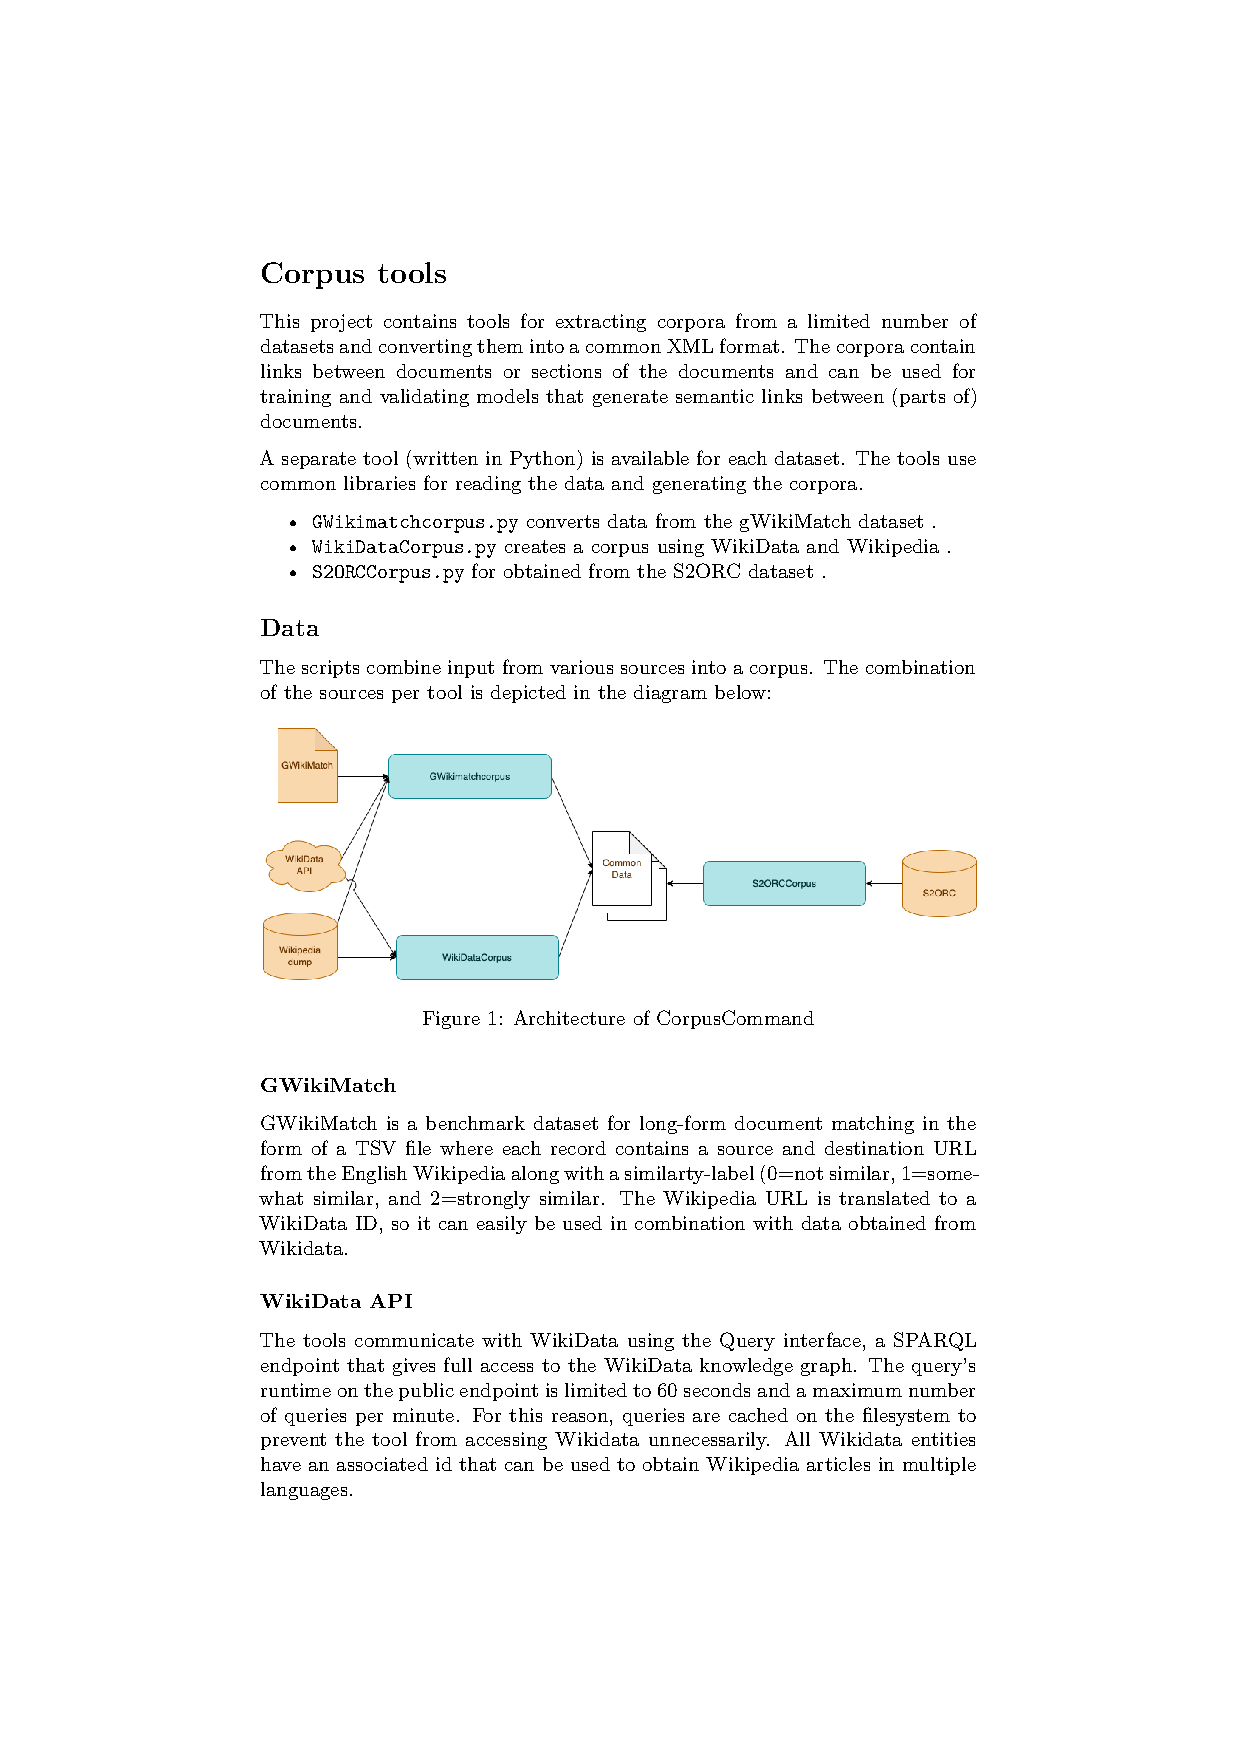
\includepdf[page=1,scale=1]{Appendices/readme.pdf}      
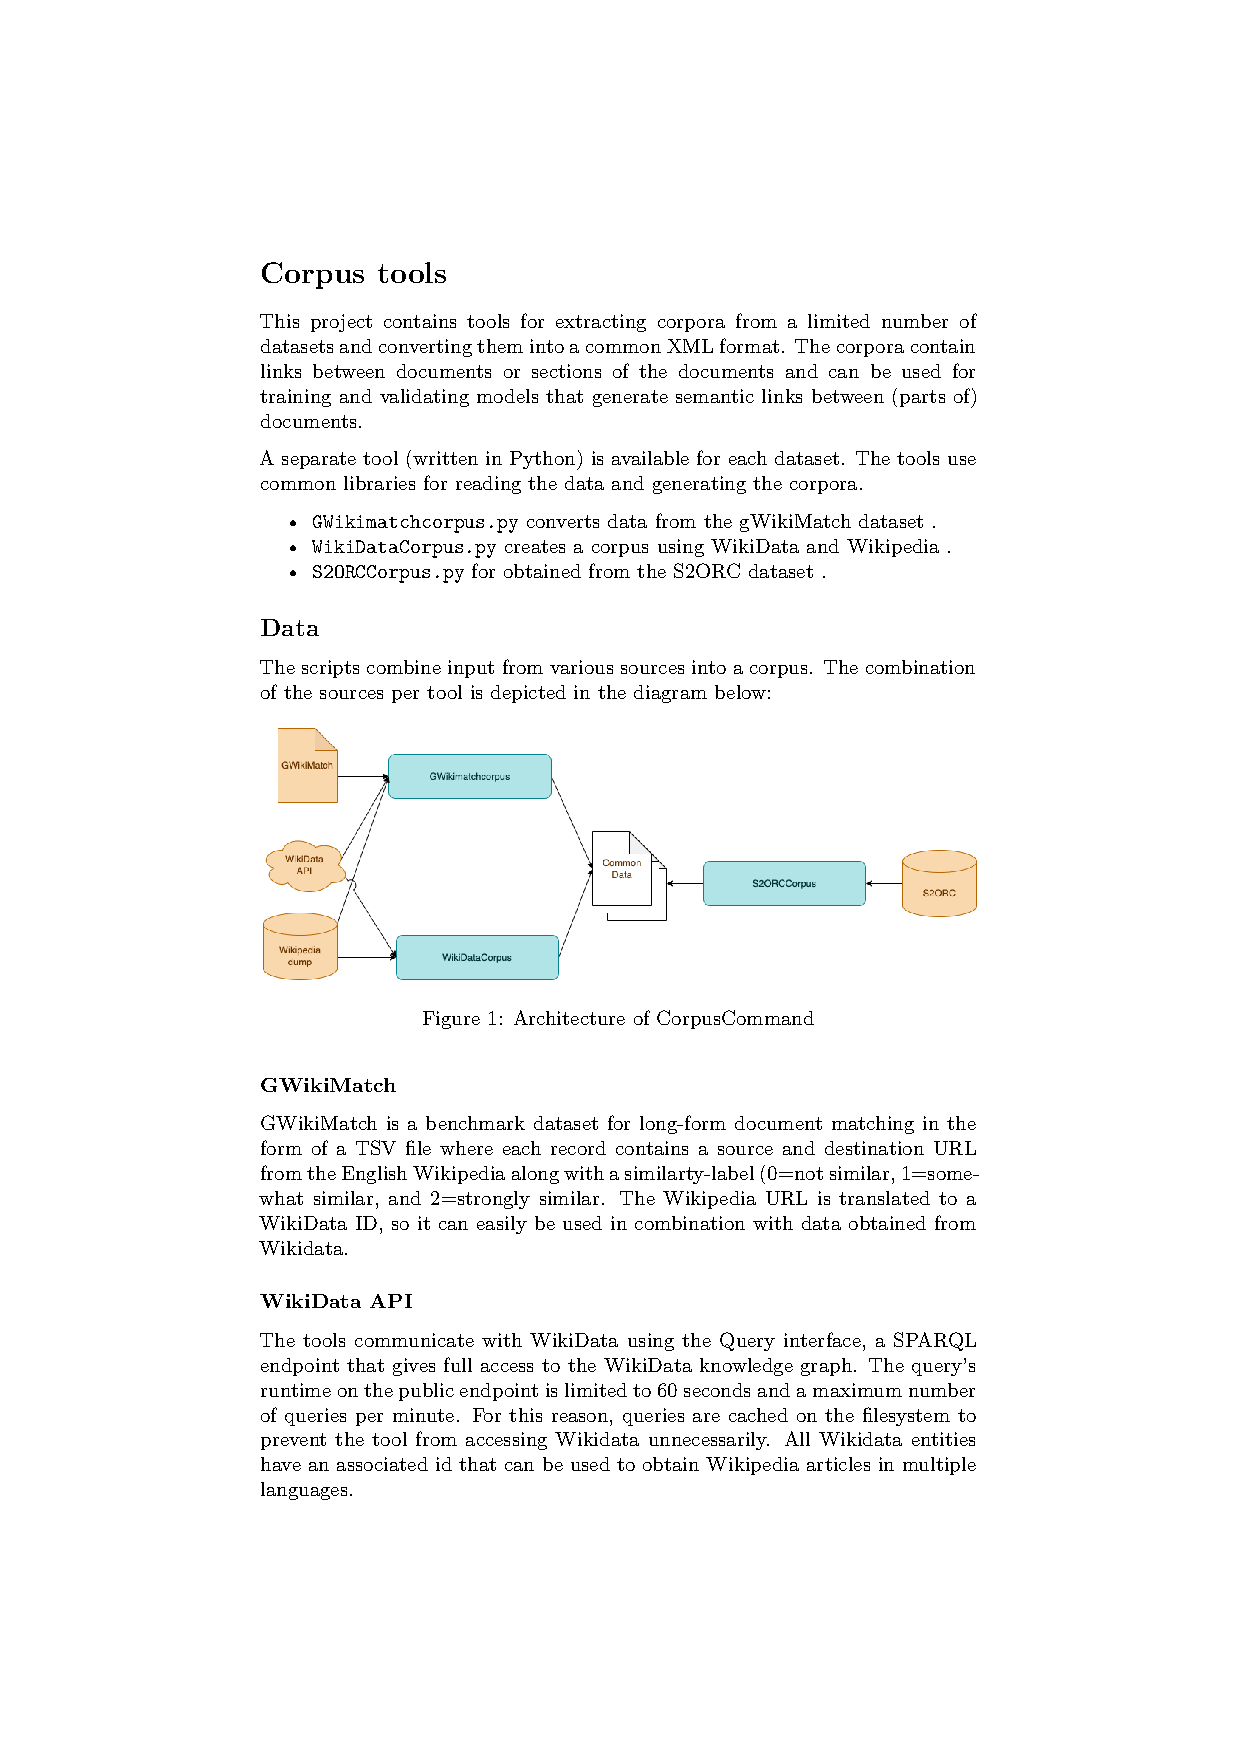
\includepdf[page=2,scale=1]{Appendices/readme.pdf}      
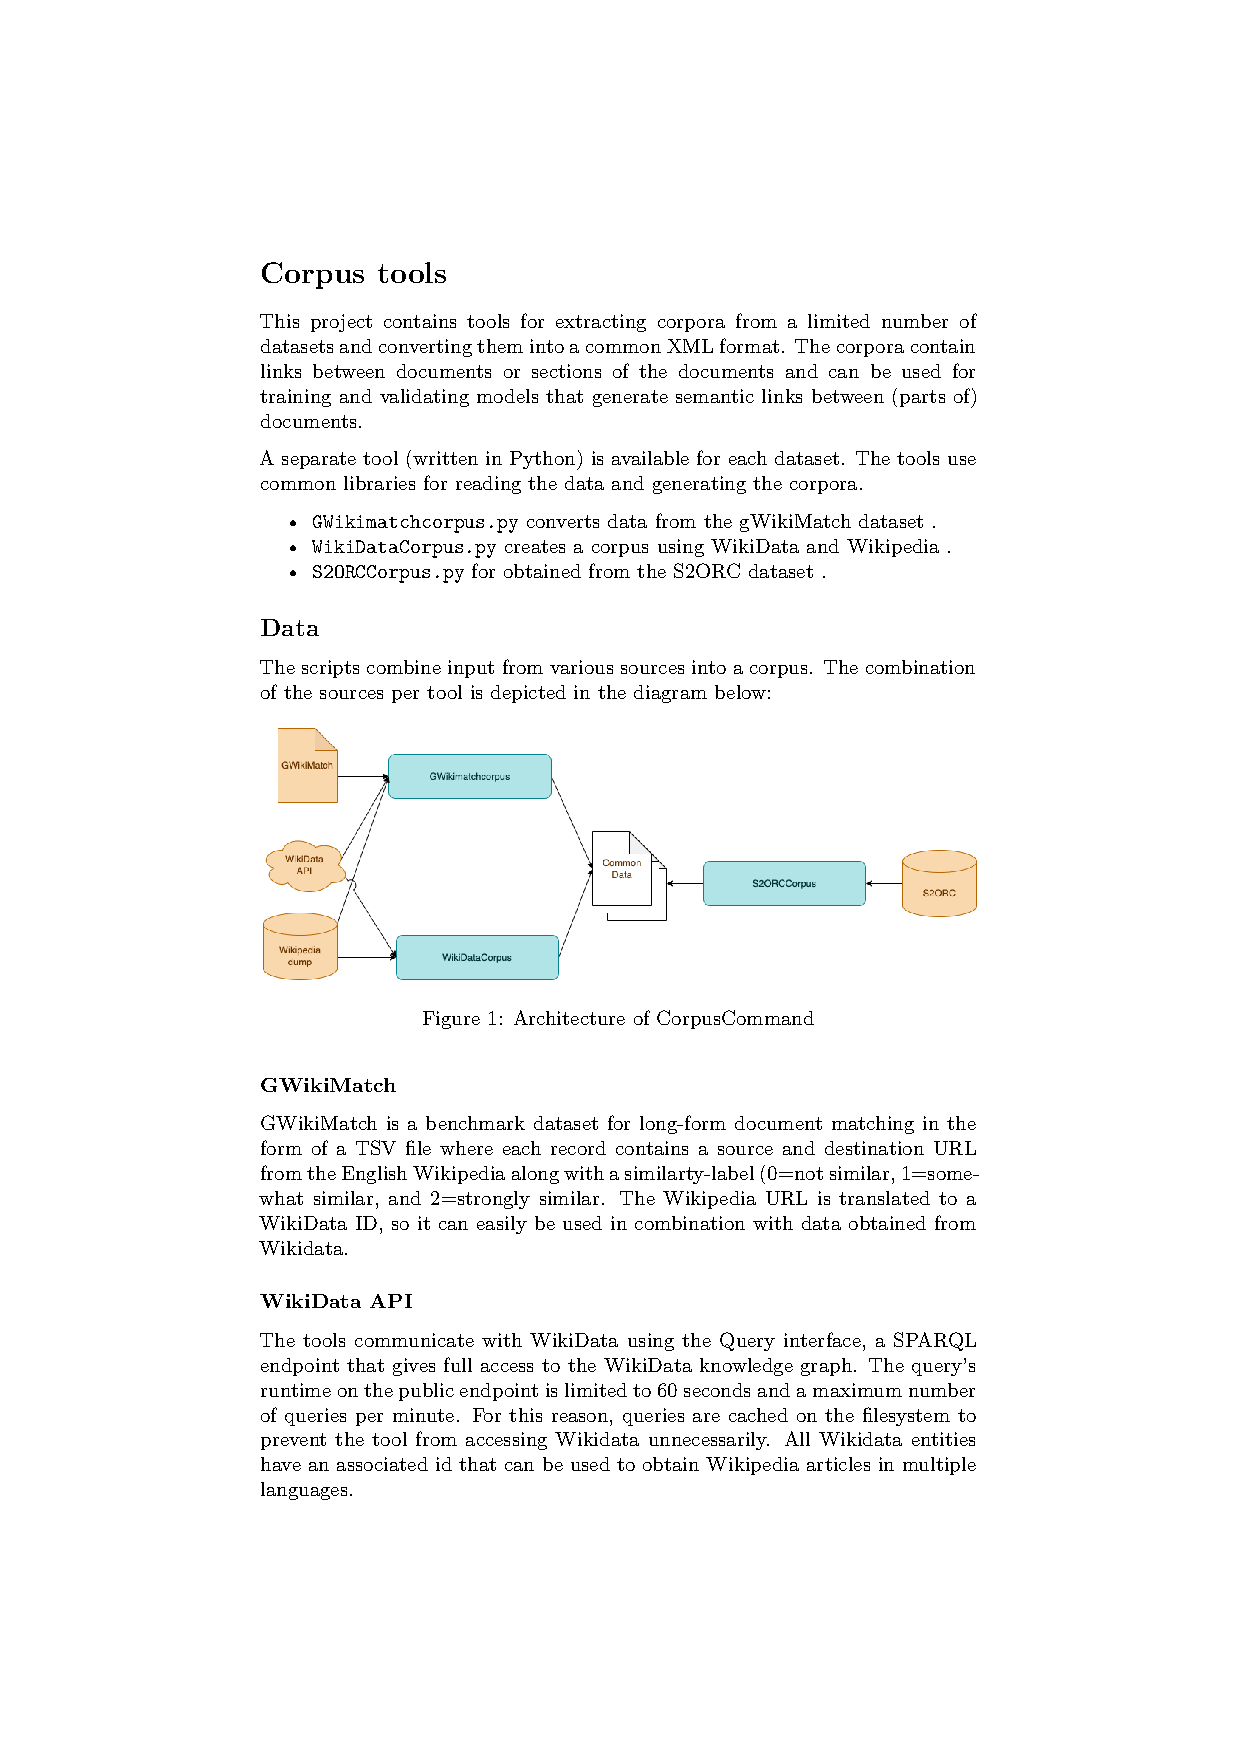
\includepdf[page=3,scale=1]{Appendices/readme.pdf}      
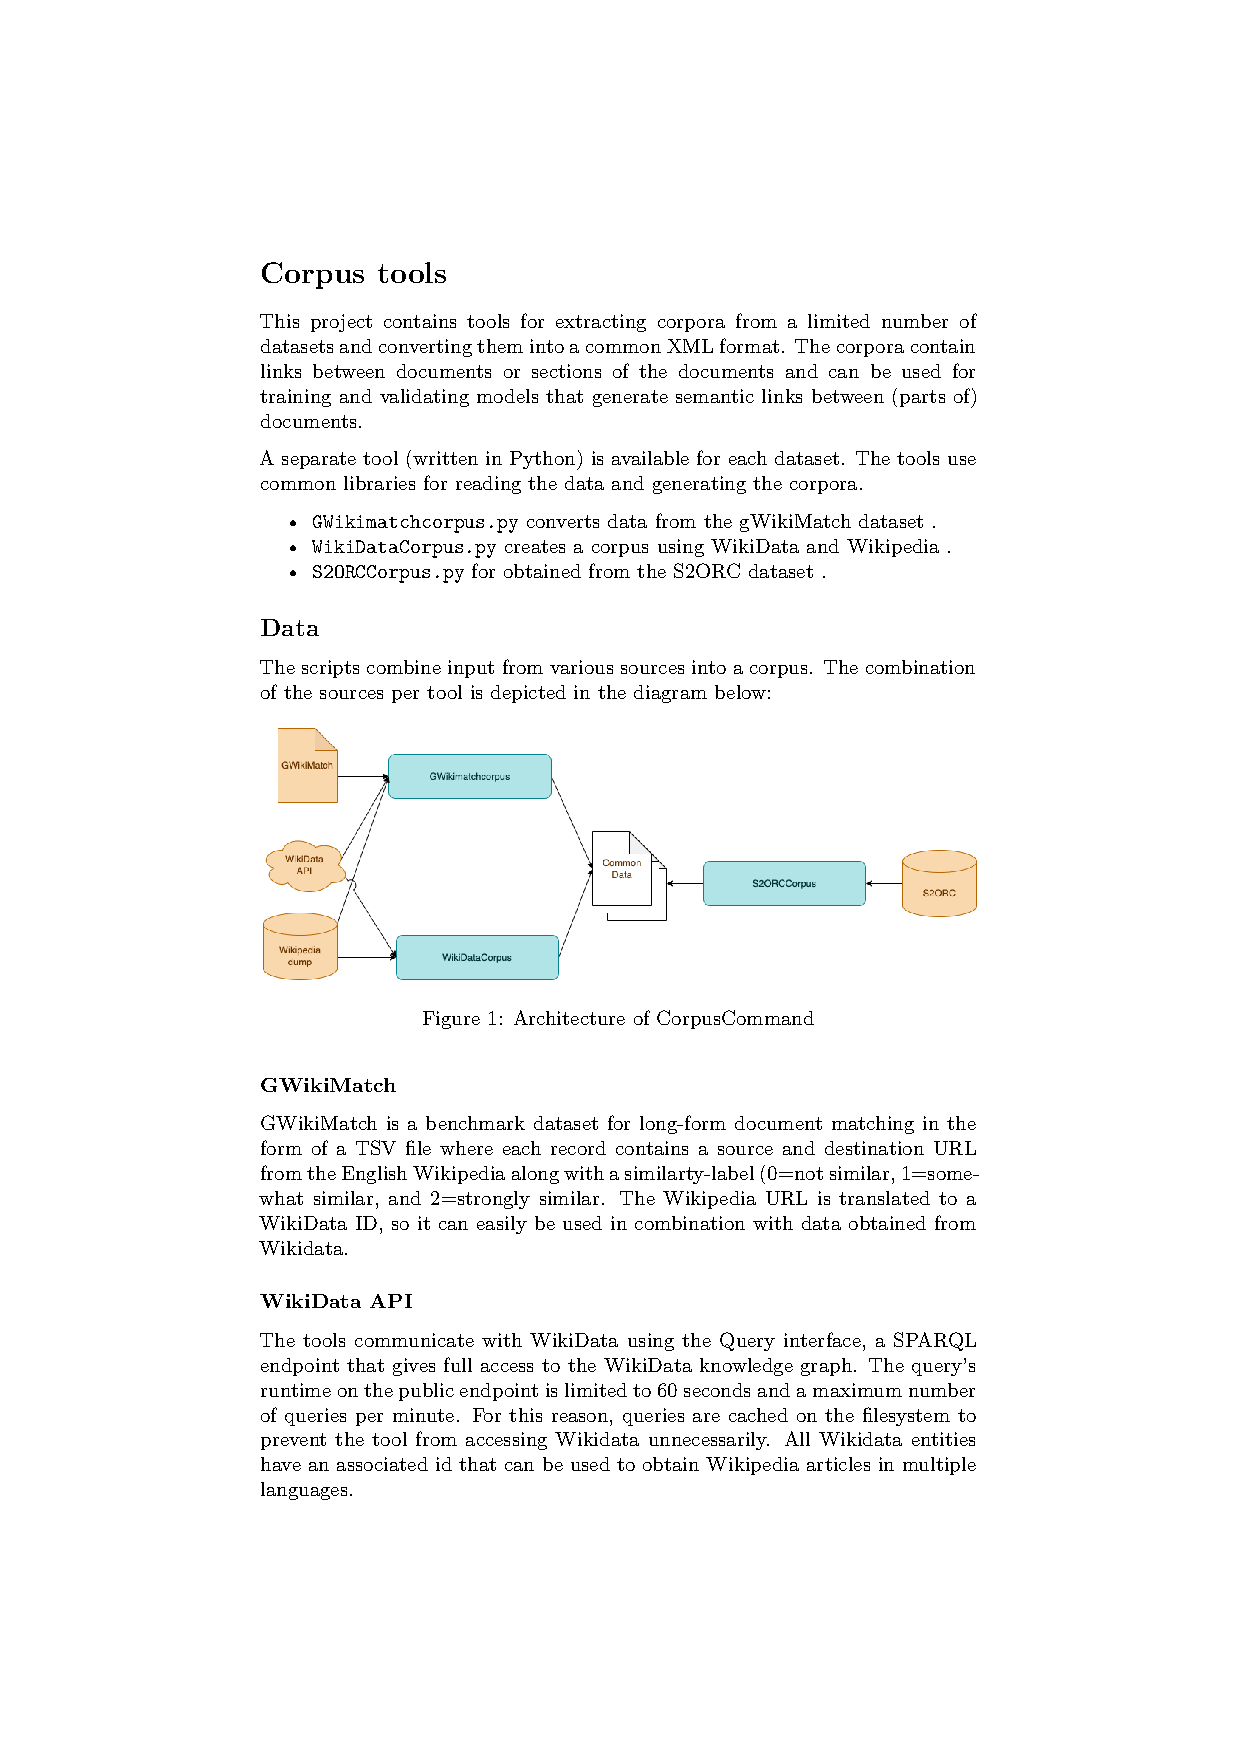
\includepdf[page=4,scale=1]{Appendices/readme.pdf}      

\appendix

\chapter{Appendix C}
\label{appendix:ReadmeII}
\section{Readme for the SADDLE tools}

\includepdf[page=1,scale=1]{Appendices/readmeII.pdf}      
\includepdf[page=2,scale=1]{Appendices/readmeII.pdf}      
\includepdf[page=3,scale=1]{Appendices/readmeII.pdf}      
\includepdf[page=4,scale=1]{Appendices/readmeII.pdf}      

\appendix

\chapter{Appendix D}
\label{appendix:ArticleParis}
\section{Article pairs}
The 46 article pairs, starting with the letter 'a' at random from Wikipedia, as used in \citep{hwang2015}. The list was composed using reverse engineering. Articles marked with * were not found in the 2014 version of the Wikipedia.\\

\begin{tabular}{lll}

Anniston, Alabama & Arovell Verlag \\
Aquarius (sports drink) & American Lacrosse Conference \\
Australia national football team & Accent \\
Advaita Vedanta & Armed Forces of the Russian Federation \\
Aegyptosaurus & Accession of Romania to the European Union \\
Andrew Huxley & Academy Award for Best Picture (1930s) * \\
Aboriginal land rights in Australia & Ashley Tisdale \\
African elephant & AAC \\
Alcina & Azuki bean \\
Anthony Wagner & A major \\
Actor & American basketball at the Olympics * \\
Academy Award for Best Picture (1950s) * & Aemilianus \\
Angers & Arsenic triiodide \\
Aspen & All For Latvia! \\
Adrian Lowe & Alchemy \\
Acherontia atropos & Alexander the Great \\
Akilattirattu Ammanai & Arrangement (music) \\
A1 Grand Prix & Absolute zero \\
Ashtown Castle & Agathis \\
Aldeburgh Festival & Aerospace engineering \\
Alphonse Mucha & Archivist \\
Alex Chernov & Atrax \\
A.C.F. Fiorentina & Adolf von Henselt \\
Arovell Verlag &   \\

\end{tabular}
\appendix

\chapter{Appendix E}
\label{appendix:scorerelation}
\section{Relation between the length of the shortest path and the validity of the relation }
This section contains all diagrams that contain the relationship between the shortest paths between two articles and the validity of the relation according to GWikiMatch as described in section \ref{secHyperlinkDistance}.

\begin{figure}[h]
\centering
\captionsetup{justification=centering}
\includegraphics[scale=0.8]{images/distance_2000.pdf}
\caption{Articles with more than 2000 hyperlinks have been removed. }
\end{figure}

\begin{figure}[h]
\centering
\captionsetup{justification=centering}
\includegraphics[scale=0.8]{images/distance_1600.pdf}
\caption{Articles with more than 1600 hyperlinks have been removed. }
\end{figure}

\begin{figure}[h]
\centering
\captionsetup{justification=centering}
\includegraphics[scale=0.8]{images/distance_1200.pdf}
\caption{Articles with more than 1200 hyperlinks have been removed. }
\end{figure}

\begin{figure}[h]
\centering
\captionsetup{justification=centering}
\includegraphics[scale=0.8]{images/distance_800.pdf}
\caption{Articles with more than 800 hyperlinks have been removed. }
\end{figure}

\begin{figure}[h]
\centering
\captionsetup{justification=centering}
\includegraphics[scale=0.8]{images/distance_400.pdf}
\caption{Articles with more than 400 hyperlinks have been removed. }
\end{figure}

\begin{figure}[h]
\centering
\captionsetup{justification=centering}
\includegraphics[scale=0.8]{images/distance_200.pdf}
\caption{Articles with more than 200 hyperlinks have been removed. }
\end{figure}


\appendix

\appendix 

\chapter{Appendix F}
\label{appendix:appSectioncutoff}
\section{Number of sections per document }

The second column of Table \ref{tabSectioncutoff} contains what percentage of the sections will be higher than the maximum number of sections in the first column. This can be used to determine how many sections are minimally required for the SADDLE neural network.
\begin{table}[!ht]
    \centering
\captionsetup{justification=centering}
    \begin{tabular}{|l|l|}
    \hline
        Maximum number of sections & Percentage \\ \hline
4 & 68\% \\ \hline
5 & 43\% \\ \hline
6 & 31\% \\ \hline
7 & 24\% \\ \hline
8 & 19\% \\ \hline
9 & 16\% \\ \hline
10 & 14\% \\ \hline
11 & 12\% \\ \hline
12 & 10\% \\ \hline
13 & 9\% \\ \hline
14 & 8\% \\ \hline
15 & 8\% \\ \hline
16 & 7\% \\ \hline
17 & 6\% \\ \hline
18 & 5\% \\ \hline
19 & 5\% \\ \hline
20 & 4\% \\ \hline
21 & 4\% \\ \hline
22 & 4\% \\ \hline
23 & 3\% \\ \hline
24 & 3\% \\ \hline
25 & 2\% \\ \hline
26 & 2\% \\ \hline
27 & 2\% \\ \hline
28 & 2\% \\ \hline
29 & 2\% \\ \hline
30 & 2\% \\ \hline
    \end{tabular}
        \caption{Percentage of the sections will be higher than the number maximum number of sections.}
	\label{tabSectioncutoff}
\end{table}

\appendix 

\chapter{Appendix G}
\label{appendix:appSQL}
\section{Maximum F1 per corpus, language and algorithm}
\label{appSQLQueries}

Table \ref{tabMaxF1} contains the maximum values of F1 per language, corpus, and method, together with the hyperparameters that were used to obtain this value for F1. The optimal hyperparameters for evaluating iterations 1, 2, and 3 were done with this table.\\


\begin{table}[!ht]
	\centering
	\captionsetup{justification=centering}
    \begin{tabular}{l|l|l|l|l|l|l}
    \hline
        \textbf{Lang} & \textbf{Corpus} & \textbf{Method} & \textbf{NN} & \textbf{Hyperparameters} & \textbf{F1} & \textbf{\% incr.} \\ \hline
en & Wikisim & SBERT & plain & 70/30/30/12/20/200/0.1 & 0.96 & 120 \\ \hline
en & Wikisim & SBERT & stat & 80/50/10/12/50/10/0.01 & 0.66 & 82 \\ \hline
en & Wikisim & Sent2Vec & plain & 80/50/30/12/50/200/0.01 & 0.85 & 110 \\ \hline
en & Wikisim & Sent2Vec & stat & 80/40/10/12/100/10/0.001 & 0.66 & 85 \\ \hline
en & Wikisim & use & plain & 30/40/10/9/20/200/0.01 & 0.94 & 124 \\ \hline
en & Wikisim & use & stat & 80/30/10/12/50/10/0.001 & 0.66 & 87 \\ \hline
en & Wikisim & Word2Vec & plain & 80/20/20/12/100/200/0.01 & 0.84 & 111 \\ \hline
en & Wikisim & Word2Vec & stat & 80/30/10/12/100/10/0.001 & 0.66 & 88 \\ \hline
en & WiRe & SBERT & plain & 80/30/10/12/50/200/0.01 & 0.94 & 120 \\ \hline
en & WiRe & SBERT & stat & 80/50/10/12/100/10/0.001 & 0.68 & 87 \\ \hline
en & WiRe & Sent2Vec & plain & 30/30/30/12/50/200/0.01 & 0.81 & 110 \\ \hline
en & WiRe & Sent2Vec & stat & 80/50/10/12/100/10/0.001 & 0.68 & 93 \\ \hline
en & WiRe & use & plain & 80/50/20/12/100/200/0.01 & 0.88 & 116 \\ \hline
en & WiRe & use & stat & 80/50/10/12/100/10/0.01 & 0.68 & 90 \\ \hline
en & WiRe & Word2Vec & plain & 70/30/30/12/100/60/0.01 & 0.79 & 104 \\ \hline
en & WiRe & Word2Vec & stat & 80/50/10/9/100/10/0.001 & 0.68 & 90 \\ \hline
nl & Wikisim & SBERT & plain & 50/40/20/9/100/200/0.1 & 0.94 & 119 \\ \hline
nl & Wikisim & SBERT & stat & 80/50/10/12/100/10/0.001 & 0.66 & 84 \\ \hline
nl & Wikisim & Sent2Vec & plain & 50/20/30/12/20/200/0.01 & 0.93 & 128 \\ \hline
nl & Wikisim & Sent2Vec & stat & 80/40/10/9/100/10/0.001 & 0.66 & 91 \\ \hline
nl & Wikisim & use & plain & 30/30/20/12/50/200/0.1 & 0.94 & 114 \\ \hline
nl & Wikisim & use & stat & 80/40/10/12/50/10/0.001 & 0.66 & 80 \\ \hline
nl & Wikisim & Word2Vec & plain & 70/20/30/9/100/200/0.01 & 0.83 & 113 \\ \hline
nl & Wikisim & Word2Vec & stat & 80/40/10/12/20/100/0.1 & 0.66 & 90 \\ \hline
nl & WiRe & SBERT & plain & 80/50/30/12/20/200/0.1 & 0.88 & 112 \\ \hline
nl & WiRe & SBERT & stat & 80/50/10/9/100/10/0.001 & 0.68 & 86 \\ \hline
nl & WiRe & Sent2Vec & plain & 50/20/10/12/50/200/0.01 & 0.79 & 116 \\ \hline
nl & WiRe & Sent2Vec & stat & 80/50/10/9/100/10/0.01 & 0.68 & 100 \\ \hline
nl & WiRe & use & plain & 50/50/10/12/20/200/0.01 & 0.88 & 115 \\ \hline
nl & WiRe & use & stat & 80/50/10/9/100/10/0.001 & 0.68 & 89 \\ \hline
nl & WiRe & Word2Vec & plain & 30/50/30/12/50/200/0.01 & 0.74 & 105 \\ \hline
nl & WiRe & Word2Vec & stat & 80/50/10/12/20/10/0.1 & 0.68 & 97 \\ \hline
    \end{tabular}
    \caption{The column "Hyperparameters" contains the following values: Similarity/Maxdoc/Nearest Neighbors/Sections/Batch size/Epochs/Learning rate. Column "\% incr." contains the percentual increase in F1 compared to the baseline measurement.}
    \label{tabMaxF1}
\end{table}


\section{SQL queries}
This section contains the SQL queries that were used to obtain the results from the PostgreSQL database.\\

\begin{verbatim}
/* 
   Create a view that selects the most optimal results using 
   the embeddings by language, corpus and embedding method 
*/
create or replace view best_embeddings as
select *
from  embeddings e
where not exists (
    select *
    from   embeddings lg
    where  lg.Language = e.Language 
    and    lg.corpus  = e.corpus 
    and    lg.method = e.Method 
    and    lg.f1 > e.f1
 );



/* Query to select the values of using the embeddings on the document */
select language Lang,
       corpus Corpus,
       method Method,
       round(cast( f1 as numeric), 2) F1,
       round( cast( accuracy as numeric), 2) Accuracy
from best_embeddings
order by language, corpus, method
\end{verbatim}
\pagebreak
\begin{verbatim}

/* Query to select results for iterations, generates a LateX table body */
    with maxF1( language, method, nntype, f1)
    as (select language, method, nntype, max(f1)
        from "resultsK5"
        group by language, method, nntype
        order by 1, 2, 3)
    select  r.language || ' & ' || r.corpus || ' & ' || r.method || ' & ' ||
            r.similarity || '/' || r.maxdoc || '/' || r.nn || '/' || r.n ||  '/' || r.batchsize || '/' || r.epochs || '/' || r.learningrate
            || ' & ' ||  round( cast( r.f1 as numeric), 2)
            || ' \\ \hline'
    from maxF1 m inner join "resultsK5" r on(
        m.language = r.language
        and    m.nntype = r.nntype
        and    m.method = r.method
        and    m.f1     = r.f1
        and not exists(
            select *
            from "resultsK5" s
            where s.language = r.language
                and    s.nntype = r.nntype
                and    s.method = r.method
                and    s.f1     = r.f1
                and    s.index > r.index
        )
    )
        inner join best_embeddings e on (
            e.language = r.language
        and e.corpus = r.corpus
        and e.method = r.method)
    order by r.language, r.method, r.nntype, r.f1


/* Query to select the results, nntype and method can be different */
    select  r.language || ' & ' || r.corpus || ' & ' || r.method
            || ' & ' ||  round( cast( r.f1 as numeric), 2)
            || ' & ' ||  round( cast( r.accuracy as numeric), 2)
            || ' & ' ||  round( cast( e.f1 as numeric), 2)
            || ' & ' ||  round( cast( e.accuracy as numeric), 2)
            || ' \\ \hline'
    from "resultsK5" r inner join best_embeddings e
            on (r.language = e.language and r.corpus = e.corpus
                and r.method = e.method)
    where r.similarity = 30
    and   r.maxdoc = 40
    and   r.nn = 20
    and   r.n = 9
    and   r.batchsize = 50
    and   r.epochs = 100
    and   r.learningrate = 0.1
    and   r.nntype = 'plain'
    and   r.method in ('Sent2Vec', 'Word2Vec')
order by r.language, r.corpus, r.method


/* Select the average training F1 and accuracy compared to the base 
   The output is formatted as a Latex table */



SELECT
    r.language || ' & ' || r.corpus || ' & ' || r.method || ' & ' || r.nntype
            || ' & ' ||  round( cast( avg(r.f1) as numeric), 2)
            || ' & ' ||  round( cast( avg(r.accuracy) as numeric), 2)
            || ' & ' ||  round( cast( avg( e.f1) as numeric), 2)
            || ' & ' ||  round( cast( avg( e.accuracy) as numeric), 2)
            || ' & ' ||  CASE WHEN avg(r.f1) > avg(e.f1) THEN '+' ELSE '-' END

            || ' \\ \hline'

FROM "resultsTT" r INNER JOIN embeddings e ON (
            e.language = r.language
        AND r.method = e.method
        AND r.corpus = e.corpus
    )
WHERE r.f1 > 0.5
GROUP BY r.language, r.nntype, r.method, r.corpus






/* Fill the sizes of the document pairs per corpus and language */
insert into pairs( corpus, language, count) values( 'Wikisim', 'nl', 203);
insert into pairs( corpus, language, count) values( 'Wikisim', 'en', 256);
insert into pairs( corpus, language, count) values( 'WiRe', 'en', 426);
insert into pairs( corpus, language, count) values( 'WiRe', 'nl', 310);
insert into pairs( corpus, language, count) values( 'gwikimatch', 'nl', 13174);
insert into pairs( corpus, language, count) values( 'gwikimatch', 'nl', 2918);
\end{verbatim}




\appendix 

\chapter{Appendix 8}
\section{Output of neural network}
\label{appendix:insightModel}

Tables \ref{tabInsightModel1} and  \ref{tabInsightModel2} contain a high-level analysis of the neural network created in phase 3 of SADDLE. The input for the neural network is an artificial vector that contains the similarities between sections. The values in this vector can either be high (0.8-1.0), medium(0.2-0.8), or low(0-0.2). The vector is initialized with low values. Column one of the table indicates the location of the values in the vector. Column two contains the values these sections are filled with high or medium values in the locations in the vector. The location of the affected sections can be at the start, middle, or end of the document (column three). Column four contains the number of sections each selected section is connected to. The last column contains the output score of the network. \\


\begin{table}[!ht]
    \begin{tabular}{l|l|l|l|l}
    \centering
    \captionsetup{justification=centering}
    \hline
        \textbf{Position} & \textbf{Values} & \textbf{Sections} & \textbf{Connected to} & \textbf{Score}  \\ \hline
None & - & none & - & 0.34\\ \hline
None & - & none & - & 0.31\\ \hline
All & high & all & 1 & 1.0\\ \hline
All & high & all & 2 & 1.0\\ \hline
All & high & all & 3 & 1.0\\ \hline
All & high & all & 4 & 1.0\\ \hline
All & high & all & 5 & 1.0\\ \hline
All & high & all & 6 & 1.0\\ \hline
All & high & all & 7 & 1.0\\ \hline
All & high & all & 8 & 1.0\\ \hline
Start & high & 2 & 1 & 1.0\\ \hline
Start & high & 3 & 1 & 1.0\\ \hline
Start & high & 3 & 2 & 1.0\\ \hline
Start & high & 4 & 1 & 1.0\\ \hline
Start & high & 4 & 2 & 1.0\\ \hline
Start & high & 4 & 3 & 1.0\\ \hline
Middle & high & 2 & 1 & 0.0\\ \hline
Middle & high & 3 & 1 & 0.0\\ \hline
Middle & high & 3 & 2 & 0.0\\ \hline
Middle & high & 4 & 1 & 0.2\\ \hline
Middle & high & 4 & 2 & 0.0\\ \hline
Middle & high & 4 & 3 & 0.0\\ \hline
        \end{tabular}
    \caption{Scores of artificial vectors (1 of 2).}
    \label{tabInsightModel1}
\end{table}

\begin{table}[!ht]
    \centering
    \captionsetup{justification=centering}
    \begin{tabular}{l|l|l|l|l}
    \hline
        \textbf{Position} & \textbf{Values} & \textbf{Sections} & \textbf{Connected to} & \textbf{Score}  \\ \hline
End & high & 2 & 1 & 0.5\\ \hline
End & high & 3 & 1 & 0.75\\ \hline
End & high & 3 & 2 & 0.78\\ \hline
End & high & 4 & 1 & 0.2\\ \hline
End & high & 4 & 2 & 0.07\\ \hline
End & high & 4 & 3 & 0.16\\ \hline
All & medium & all & 1 & 0.95\\ \hline
All & medium & all & 2 & 0.94\\ \hline
All & medium & all & 3 & 0.94\\ \hline
All & medium & all & 4 & 0.95\\ \hline
All & medium & all & 5 & 0.95\\ \hline
All & medium & all & 6 & 0.95\\ \hline
All & medium & all & 7 & 0.93\\ \hline
All & medium & all & 8 & 0.95\\ \hline
Start & medium & 2 & 1 & 0.78\\ \hline
Start & medium & 3 & 1 & 0.88\\ \hline
Start & medium & 3 & 2 & 0.87\\ \hline
Start & medium & 4 & 1 & 0.94\\ \hline
Start & medium & 4 & 2 & 0.94\\ \hline
Start & medium & 4 & 3 & 0.94\\ \hline
Middle & medium & 2 & 1 & 0.09\\ \hline
Middle & medium & 3 & 1 & 0.01\\ \hline
Middle & medium & 3 & 2 & 0.06\\ \hline
Middle & medium & 4 & 1 & 0.24\\ \hline
Middle & medium & 4 & 2 & 0.01\\ \hline
Middle & medium & 4 & 3 & 0.01\\ \hline
End & medium & 2 & 1 & 0.41\\ \hline
End & medium & 3 & 1 & 0.56\\ \hline
End & medium & 3 & 2 & 0.54\\ \hline
End & medium & 4 & 1 & 0.18\\ \hline
End & medium & 4 & 2 & 0.2\\ \hline
End & medium & 4 & 3 & 0.25\\ \hline
        
        
        \end{tabular}
    \caption{Scores of artificial vectors (2 of 2).}
    \label{tabInsightModel2}
\end{table}




%  \appendix

\chapter{Appendix B}
\label{appendix:Readme}
\section{Readme for the Corpus Tools}

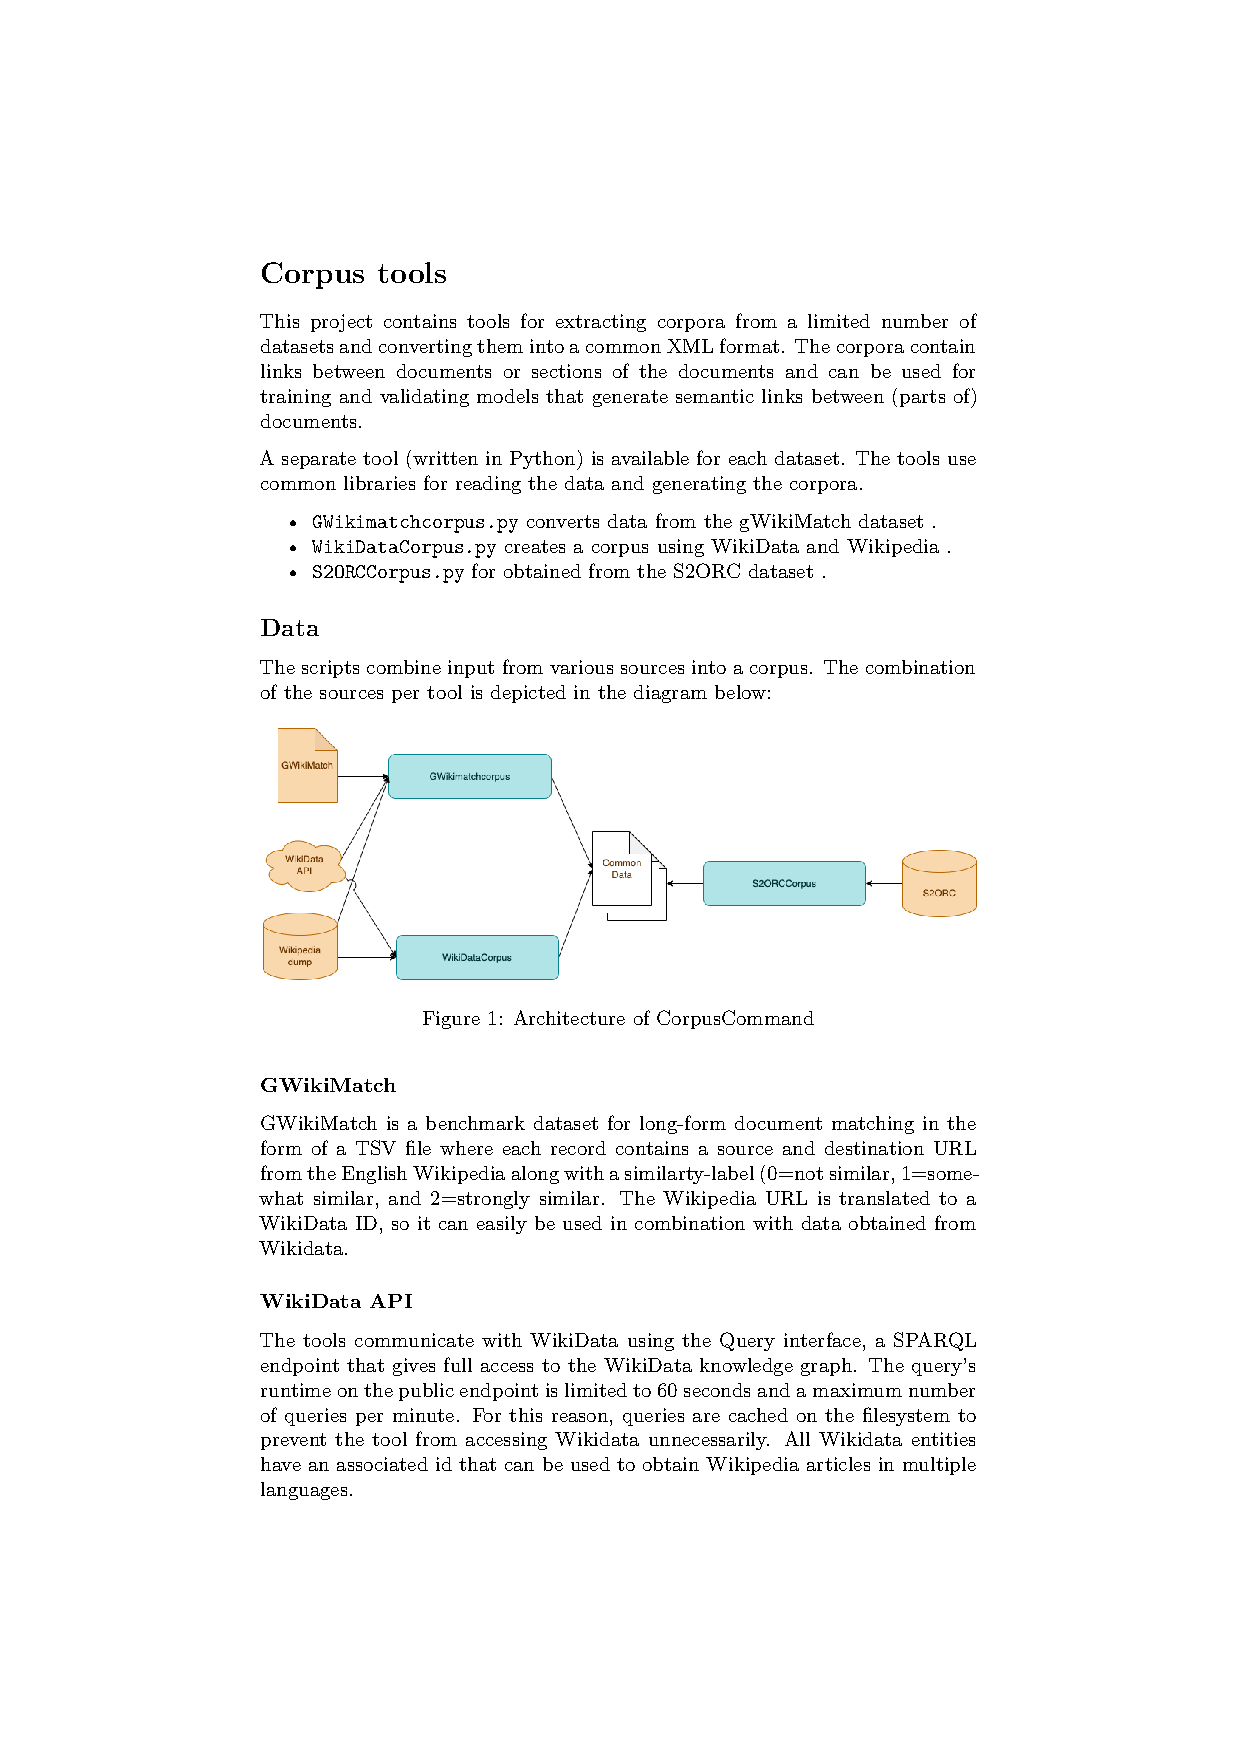
\includepdf[page=1,scale=1]{Appendices/readme.pdf}      
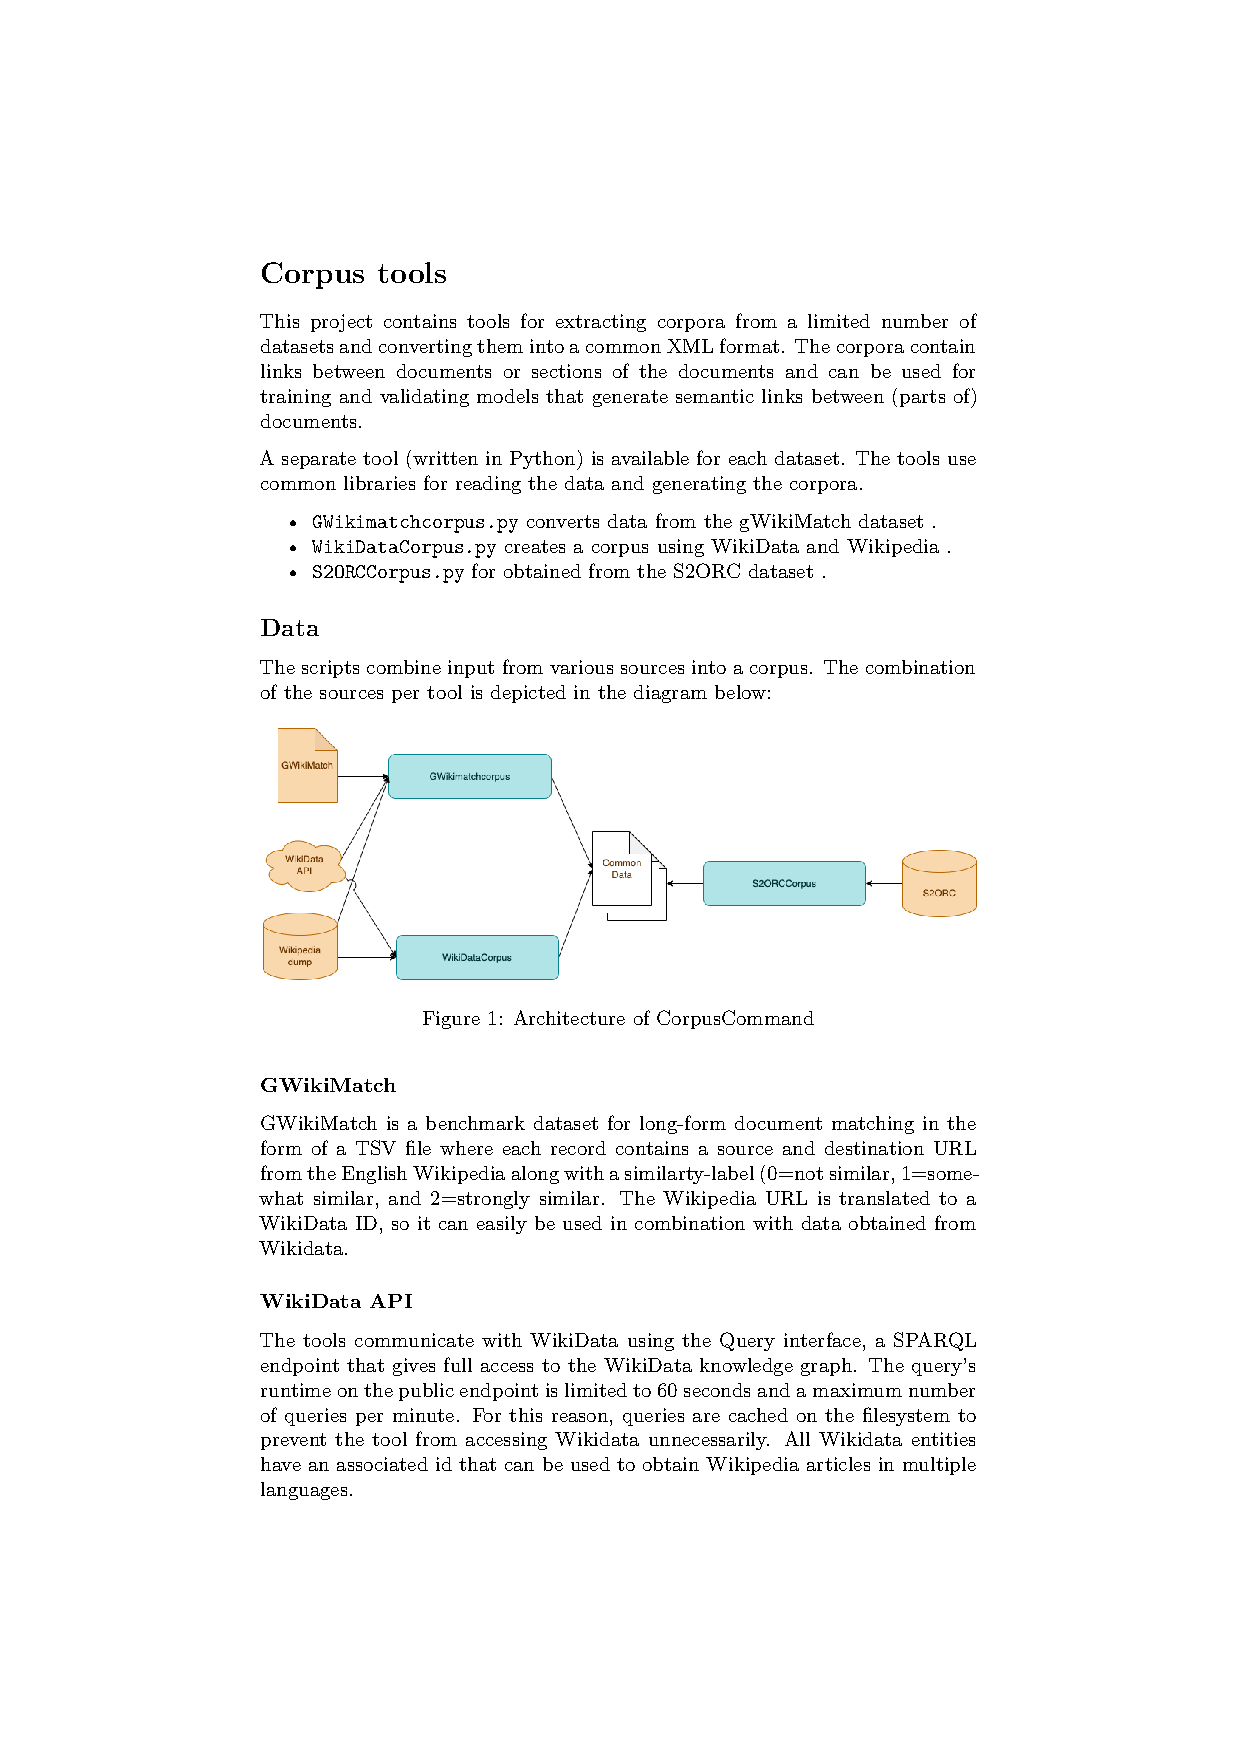
\includepdf[page=2,scale=1]{Appendices/readme.pdf}      
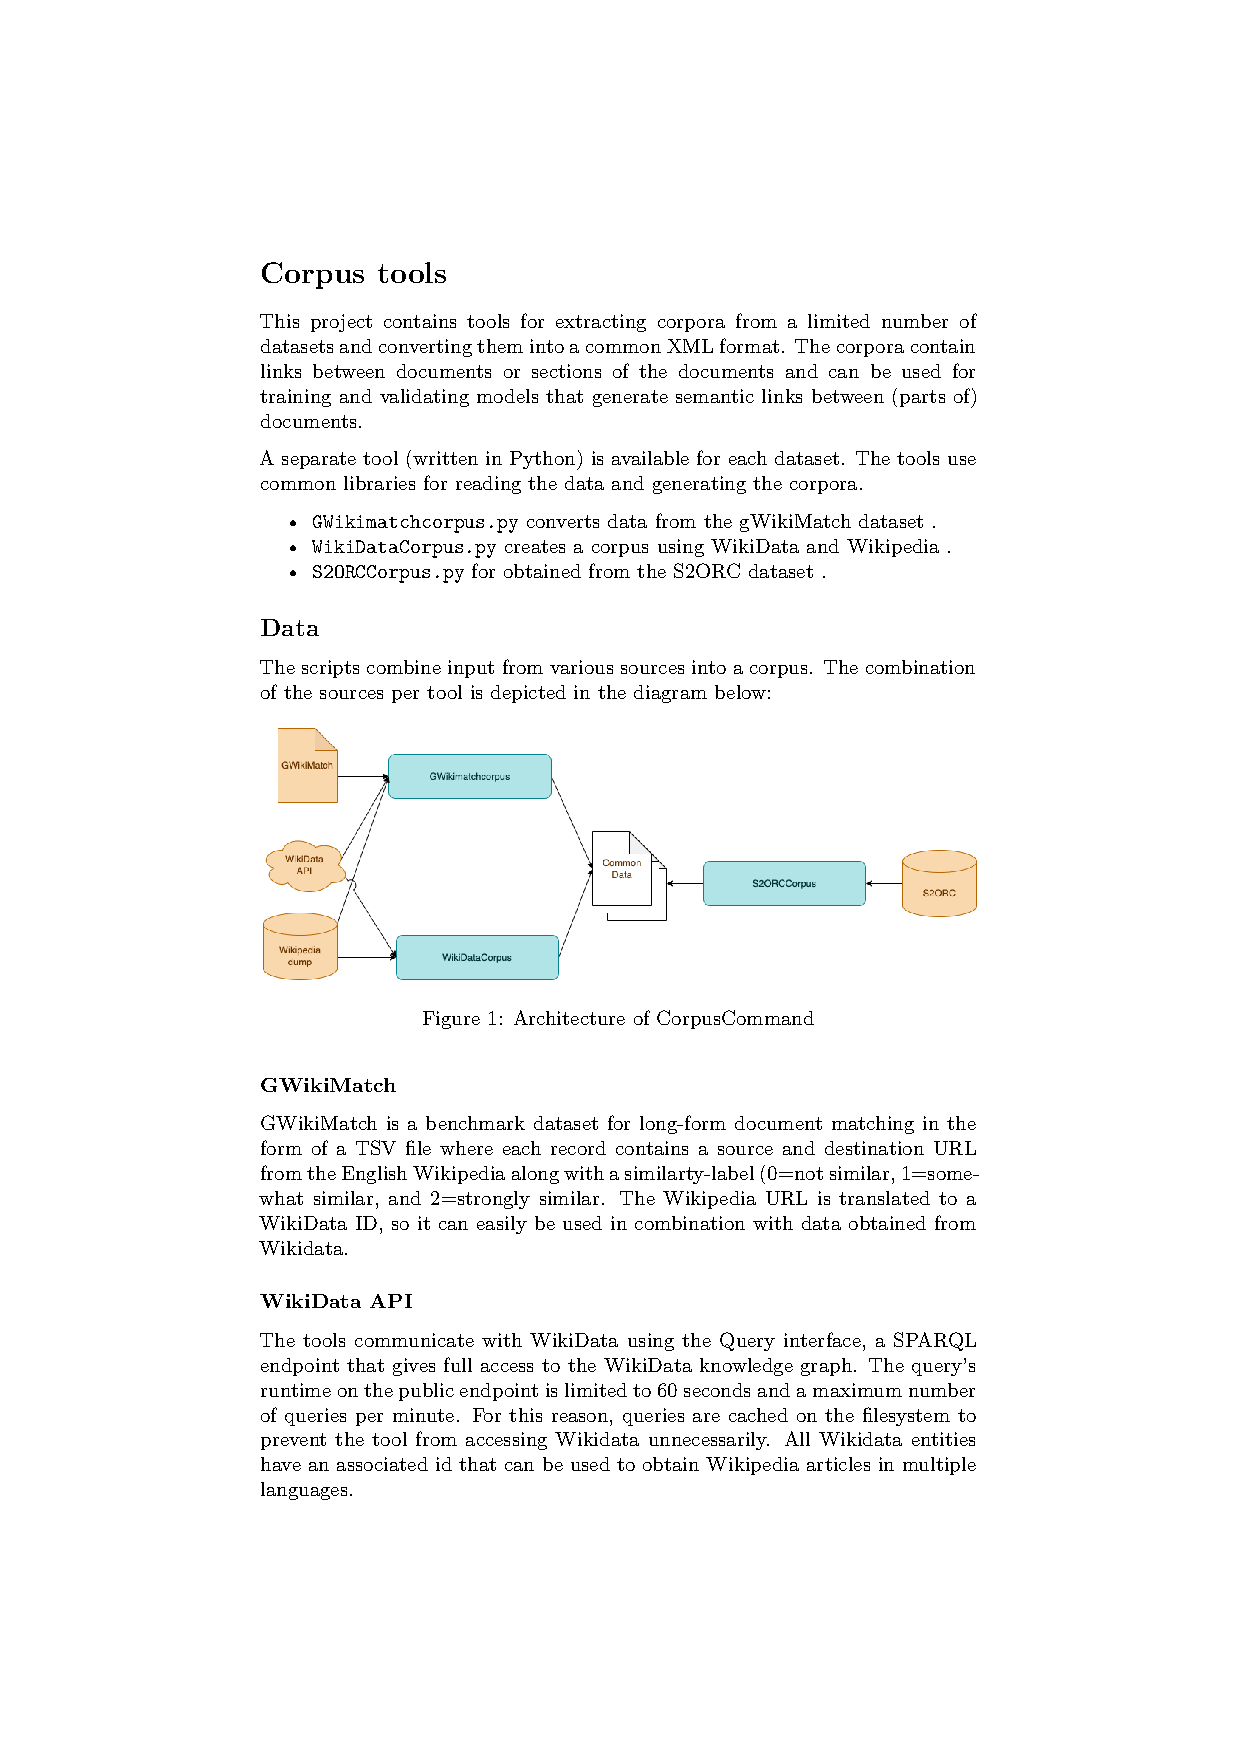
\includepdf[page=3,scale=1]{Appendices/readme.pdf}      
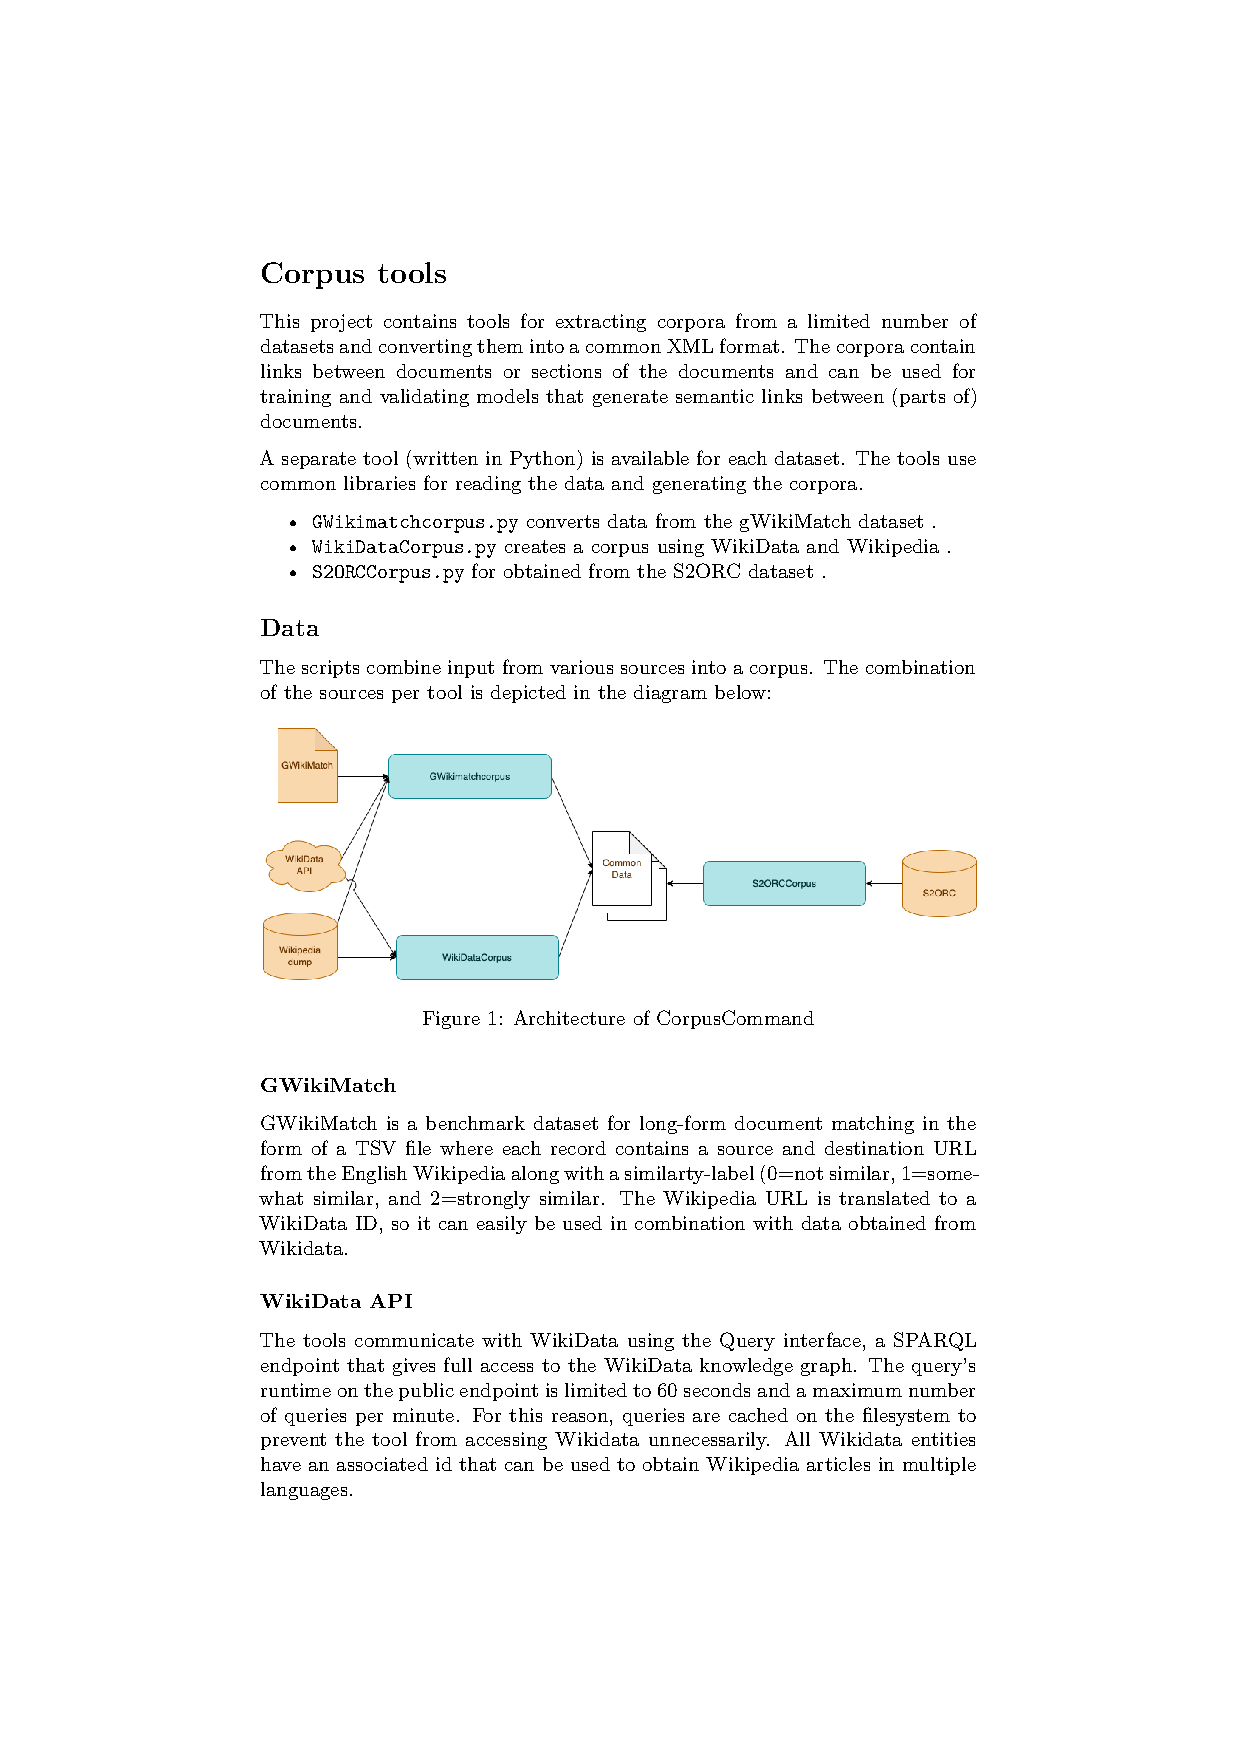
\includepdf[page=4,scale=1]{Appendices/readme.pdf}      

%  \appendix

\chapter{Appendix C}
\label{appendix:ReadmeII}
\section{Readme for the SADDLE tools}

\includepdf[page=1,scale=1]{Appendices/readmeII.pdf}      
\includepdf[page=2,scale=1]{Appendices/readmeII.pdf}      
\includepdf[page=3,scale=1]{Appendices/readmeII.pdf}      
\includepdf[page=4,scale=1]{Appendices/readmeII.pdf}      



\end{document}
